\documentclass[]{book}
\usepackage{lmodern}
\usepackage{amssymb,amsmath}
\usepackage{ifxetex,ifluatex}
\usepackage{fixltx2e} % provides \textsubscript
\ifnum 0\ifxetex 1\fi\ifluatex 1\fi=0 % if pdftex
  \usepackage[T1]{fontenc}
  \usepackage[utf8]{inputenc}
\else % if luatex or xelatex
  \ifxetex
    \usepackage{mathspec}
  \else
    \usepackage{fontspec}
  \fi
  \defaultfontfeatures{Ligatures=TeX,Scale=MatchLowercase}
\fi
% use upquote if available, for straight quotes in verbatim environments
\IfFileExists{upquote.sty}{\usepackage{upquote}}{}
% use microtype if available
\IfFileExists{microtype.sty}{%
\usepackage{microtype}
\UseMicrotypeSet[protrusion]{basicmath} % disable protrusion for tt fonts
}{}
\usepackage[margin=1in]{geometry}
\usepackage{hyperref}
\hypersetup{unicode=true,
            pdftitle={いつか役に立つかもしれない資料},
            pdfauthor={Kiri Kuroda},
            pdfborder={0 0 0},
            breaklinks=true}
\urlstyle{same}  % don't use monospace font for urls
\usepackage{natbib}
\bibliographystyle{apalike}
\usepackage{color}
\usepackage{fancyvrb}
\newcommand{\VerbBar}{|}
\newcommand{\VERB}{\Verb[commandchars=\\\{\}]}
\DefineVerbatimEnvironment{Highlighting}{Verbatim}{commandchars=\\\{\}}
% Add ',fontsize=\small' for more characters per line
\usepackage{framed}
\definecolor{shadecolor}{RGB}{248,248,248}
\newenvironment{Shaded}{\begin{snugshade}}{\end{snugshade}}
\newcommand{\KeywordTok}[1]{\textcolor[rgb]{0.13,0.29,0.53}{\textbf{#1}}}
\newcommand{\DataTypeTok}[1]{\textcolor[rgb]{0.13,0.29,0.53}{#1}}
\newcommand{\DecValTok}[1]{\textcolor[rgb]{0.00,0.00,0.81}{#1}}
\newcommand{\BaseNTok}[1]{\textcolor[rgb]{0.00,0.00,0.81}{#1}}
\newcommand{\FloatTok}[1]{\textcolor[rgb]{0.00,0.00,0.81}{#1}}
\newcommand{\ConstantTok}[1]{\textcolor[rgb]{0.00,0.00,0.00}{#1}}
\newcommand{\CharTok}[1]{\textcolor[rgb]{0.31,0.60,0.02}{#1}}
\newcommand{\SpecialCharTok}[1]{\textcolor[rgb]{0.00,0.00,0.00}{#1}}
\newcommand{\StringTok}[1]{\textcolor[rgb]{0.31,0.60,0.02}{#1}}
\newcommand{\VerbatimStringTok}[1]{\textcolor[rgb]{0.31,0.60,0.02}{#1}}
\newcommand{\SpecialStringTok}[1]{\textcolor[rgb]{0.31,0.60,0.02}{#1}}
\newcommand{\ImportTok}[1]{#1}
\newcommand{\CommentTok}[1]{\textcolor[rgb]{0.56,0.35,0.01}{\textit{#1}}}
\newcommand{\DocumentationTok}[1]{\textcolor[rgb]{0.56,0.35,0.01}{\textbf{\textit{#1}}}}
\newcommand{\AnnotationTok}[1]{\textcolor[rgb]{0.56,0.35,0.01}{\textbf{\textit{#1}}}}
\newcommand{\CommentVarTok}[1]{\textcolor[rgb]{0.56,0.35,0.01}{\textbf{\textit{#1}}}}
\newcommand{\OtherTok}[1]{\textcolor[rgb]{0.56,0.35,0.01}{#1}}
\newcommand{\FunctionTok}[1]{\textcolor[rgb]{0.00,0.00,0.00}{#1}}
\newcommand{\VariableTok}[1]{\textcolor[rgb]{0.00,0.00,0.00}{#1}}
\newcommand{\ControlFlowTok}[1]{\textcolor[rgb]{0.13,0.29,0.53}{\textbf{#1}}}
\newcommand{\OperatorTok}[1]{\textcolor[rgb]{0.81,0.36,0.00}{\textbf{#1}}}
\newcommand{\BuiltInTok}[1]{#1}
\newcommand{\ExtensionTok}[1]{#1}
\newcommand{\PreprocessorTok}[1]{\textcolor[rgb]{0.56,0.35,0.01}{\textit{#1}}}
\newcommand{\AttributeTok}[1]{\textcolor[rgb]{0.77,0.63,0.00}{#1}}
\newcommand{\RegionMarkerTok}[1]{#1}
\newcommand{\InformationTok}[1]{\textcolor[rgb]{0.56,0.35,0.01}{\textbf{\textit{#1}}}}
\newcommand{\WarningTok}[1]{\textcolor[rgb]{0.56,0.35,0.01}{\textbf{\textit{#1}}}}
\newcommand{\AlertTok}[1]{\textcolor[rgb]{0.94,0.16,0.16}{#1}}
\newcommand{\ErrorTok}[1]{\textcolor[rgb]{0.64,0.00,0.00}{\textbf{#1}}}
\newcommand{\NormalTok}[1]{#1}
\usepackage{longtable,booktabs}
\usepackage{graphicx,grffile}
\makeatletter
\def\maxwidth{\ifdim\Gin@nat@width>\linewidth\linewidth\else\Gin@nat@width\fi}
\def\maxheight{\ifdim\Gin@nat@height>\textheight\textheight\else\Gin@nat@height\fi}
\makeatother
% Scale images if necessary, so that they will not overflow the page
% margins by default, and it is still possible to overwrite the defaults
% using explicit options in \includegraphics[width, height, ...]{}
\setkeys{Gin}{width=\maxwidth,height=\maxheight,keepaspectratio}
\IfFileExists{parskip.sty}{%
\usepackage{parskip}
}{% else
\setlength{\parindent}{0pt}
\setlength{\parskip}{6pt plus 2pt minus 1pt}
}
\setlength{\emergencystretch}{3em}  % prevent overfull lines
\providecommand{\tightlist}{%
  \setlength{\itemsep}{0pt}\setlength{\parskip}{0pt}}
\setcounter{secnumdepth}{5}
% Redefines (sub)paragraphs to behave more like sections
\ifx\paragraph\undefined\else
\let\oldparagraph\paragraph
\renewcommand{\paragraph}[1]{\oldparagraph{#1}\mbox{}}
\fi
\ifx\subparagraph\undefined\else
\let\oldsubparagraph\subparagraph
\renewcommand{\subparagraph}[1]{\oldsubparagraph{#1}\mbox{}}
\fi

%%% Use protect on footnotes to avoid problems with footnotes in titles
\let\rmarkdownfootnote\footnote%
\def\footnote{\protect\rmarkdownfootnote}

%%% Change title format to be more compact
\usepackage{titling}

% Create subtitle command for use in maketitle
\newcommand{\subtitle}[1]{
  \posttitle{
    \begin{center}\large#1\end{center}
    }
}

\setlength{\droptitle}{-2em}

  \title{いつか役に立つかもしれない資料}
    \pretitle{\vspace{\droptitle}\centering\huge}
  \posttitle{\par}
    \author{Kiri Kuroda}
    \preauthor{\centering\large\emph}
  \postauthor{\par}
    \date{}
    \predate{}\postdate{}
  
\usepackage{booktabs}

\begin{document}
\maketitle

{
\setcounter{tocdepth}{1}
\tableofcontents
}
\chapter*{はじめに(服用上の注意)}
\addcontentsline{toc}{chapter}{はじめに(服用上の注意)}

\textbf{効能}:データの性質を他人にわかりやすく伝えられるようになる。

\textbf{対象}:卒論等で(コンテンツはさておいて)わかりやすく、なんとなく見栄えの良いレポート・発表をしたいと思ってはいるけれど、どこから手を着ければいいかわからない人。

\textbf{注意}:読んでいてわからないことに出くわした場合、とりあえずググってみること。おそらく検索能力も重要なスキルである。周りの人に尋ねてみるのも推奨。

\chapter*{RとRStudioのセットアップ}\label{rrstudio}
\addcontentsline{toc}{chapter}{RとRStudioのセットアップ}

以下の手順でRとRStudioをセットアップしてほしい。Rは統計ソフトウェアの本体、RStudioは「Rを使いやすくするためのソフトウェア」である。

どこかでつまずいたら、とにかく周りの人に聞いてみよう\footnote{何にでも(卒論にも)当てはまるが、自分から尋ねない限り、誰も手は差し伸べてくれないものである。逆に言えば、何か尋ねさえすれば、答えてくれない人はいないものである。}。

\section{Rのインストール}\label{r}

\url{https://cran.r-project.org}
にアクセスし、自分のパソコンのOSに合ったものをインストールする。

\section{RStudioのインストール}\label{rstudio}

\url{https://www.rstudio.com}
にアクセスし、RStudioをインストールする。インストールの際は、``Free''と書かれているものを選ぶようにすること。

\section{パッケージのインストール}

RとRStudioが揃っても、「パッケージ」というものがないと話にならない。RとRStudioをiOSやAndroidとすれば、パッケージはアプリのようなものである。パッケージのインストールは\texttt{install.packages("パッケージ名)}で実行できる。\texttt{install.packages()}は1度だけ行えば良い。

以下のコードをコンソールに入力して実行しよう。

\begin{Shaded}
\begin{Highlighting}[]
\CommentTok{# 本資料で使うパッケージのインストール}
\KeywordTok{install.packages}\NormalTok{(}\KeywordTok{c}\NormalTok{(}\StringTok{"tidyverse"}\NormalTok{,}\StringTok{"gcookbook"}\NormalTok{,}\StringTok{"GGally"}\NormalTok{,}\StringTok{"devtools"}\NormalTok{))}
\end{Highlighting}
\end{Shaded}

\section{パッケージの読み込み}

パッケージはインストールできたが、それだけでは十分ではない。RStudioを立ち上げるたびにパッケージを読み込まなくてはいけないのである。\texttt{library(パッケージ名)}でパッケージを読み込むことができる。

\begin{Shaded}
\begin{Highlighting}[]
\KeywordTok{library}\NormalTok{(tidyverse) }\CommentTok{# 例:色々メッセージが出てくるが、気にしなくて良い}
\end{Highlighting}
\end{Shaded}

\section{どうやってRのコードを実行するか?}\label{r}

R自体を立ち上げる必要はなく、RStudioを立ち上げれば本資料のコードを実行することができる。

具体的な操作方法については、文章化するのが予想以上に面倒だったので、説明は他に譲る(\ldots{}\ldots{})。たとえば、\url{https://kazutan.github.io/JSSP2018_spring/intro_rstudio.html}
が参考になるだろう。個人的には、R
Markdownという記法がレポーティングに最適だと思うが、現時点では気になる人だけ調べれば良いと思う。

\part*{データの可視化}\label{part-}
\addcontentsline{toc}{part}{データの可視化}

\chapter{可視化の重要性}\label{introduction}

\textbf{データの可視化}(≒作図)はデータ分析において不可欠である。むしろ、\textbf{統計的分析より重要}なこともしばしばである。「言うほど重要か?」と思う人がいるかもしれないので、有名な\textbf{「アンスコムの例(Anscombe's
quartet)」}を使ってそれを例証してみよう。

\section{アンスコムの例}

仮に4人の学生が同じ実験を実施したとする(それぞれ実験I, II, III,
IV)。その実験では参加者(各11名)の個人傾向を様々な尺度で測定しており、ここでは変数「x」と「y」が測定されたと考えてみてほしい(変数は別に「x」と「y」である必要はなく、「身長」と「体重」などでも良い)。

4人はそれぞれの実験における変数xとyの\textbf{平均値}(mean;
\emph{M})と\textbf{標準偏差}(standard deviation;
\emph{SD})と\textbf{相関係数}(correlation coefficient;
\emph{r})を計算し、ゼミで報告した(下の表は適当に解読してほしい)。

experiment

mean\_x

sd\_x

mean\_y

sd\_y

pearson\_r

I

9

3.316625

7.500909

2.031568

0.8164205

II

9

3.316625

7.500909

2.031657

0.8162365

III

9

3.316625

7.500000

2.030424

0.8162867

IV

9

3.316625

7.500909

2.030579

0.8165214

この表からわかるように、どの実験でもxとyの平均値、標準偏差、相関係数はほとんど同じだった。

\begin{center}\rule{0.5\linewidth}{\linethickness}\end{center}

\ldots{}\ldots{}

\textbf{という報告を私たちはついついやりがち}である。しかし、これらの報告はデータの重要な性質を見落としている。

では、ここでxとyの\textbf{散布図}を描いてみよう。

(ref:anscombe-scatter-plot)
「アンスコムの例」の散布図。どの変数も統計量(平均値、標準偏差、相関係数)の上では同じだが、実際は明らかに異なるパターンを示していることがひと目でわかる。

\begin{figure}

{\centering 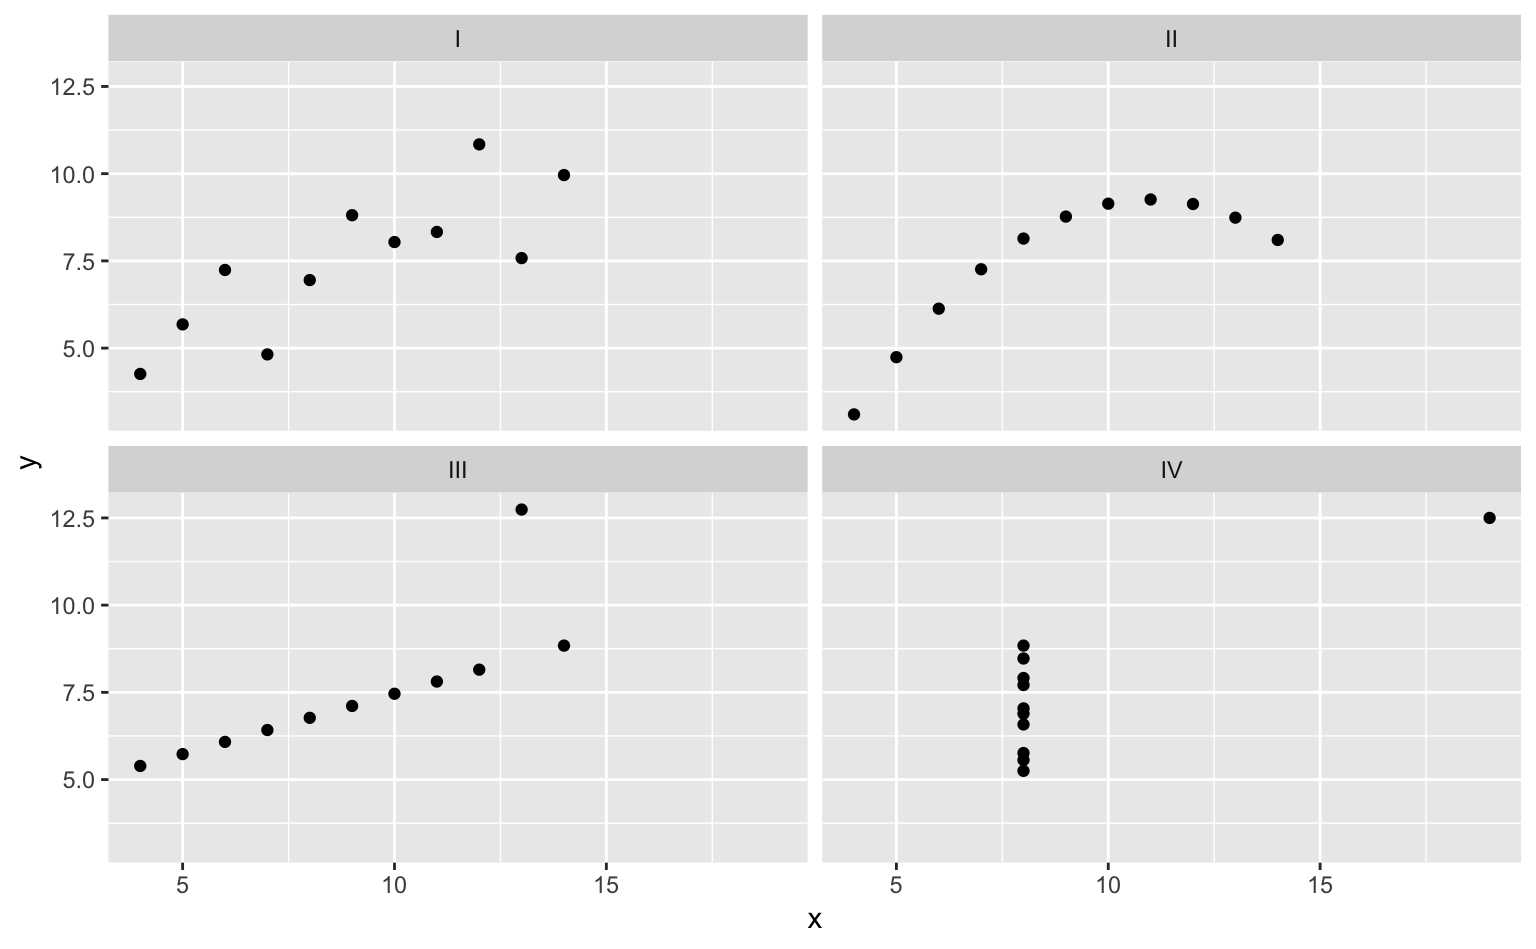
\includegraphics{lecture_note_files/figure-latex/unnamed-chunk-7-1} 

}

\caption{(ref:anscombe-scatter-plot)}\label{fig:unnamed-chunk-7}
\end{figure}

上の図を見て\textbf{ひと目でわかる}ように、xとyの平均値、標準偏差、相関係数が同じであるにもかかわらず、各実験のデータは全く異なる様相を呈していた。

このように、\textbf{可視化は非常に強力なデータ分析手法}の一つである(スプレッドシートの数字だけを見て、これらの図を頭に思い浮かべられる人はいるだろうか?)。また、この例は\textbf{可視化の本質}を私たちに教えてくれる。その本質とは、

\begin{itemize}
\item
  \textbf{変数の数量や分布}(distribution)がひと目で分かる
\item
  \textbf{変数間の関係}(association)がひと目でわかる
\end{itemize}

ということである。少し乱暴にまとめてしまうと、\textbf{グラフとは変数の分布や関係を可視化したもの}にほかならない。

「ひと目でわかる」という点も重要である。もし発表者が表や統計量だけを見せ、それをもとに議論を始めたら、あなたはどのように感じるだろうか? 数字ばかり見せられた聴衆は話をフォローできなくなるし、そもそも最初から聞く耳を持たなくなってしまう場合もある。\textbf{ヒトの認知資源には限りがあるし、わかりにくい話にずっと耳を貸していられるほど人々は親切でもない}と思っておいたほうが賢明だろう。

とにかく、まずは黙って\textbf{「可視化からはじめよ」}を肝に銘じてほしい。

\section{可視化のツール:ggplot2}\label{ggplot2}

さて、データ分析+論文用の可視化には\textbf{R}という統計ソフトの\textbf{ggplot2}というパッケージ(\textbf{tidyverse}というパッケージ群の1つ)が便利である。逆に言えば、tidyverseやggplot2がなければRを使うメリットは見いだせないと言っても過言ではない。

ggplot2がなぜ便利なのかを一言で説明するのは難しいが、なぜ他のツールーーたとえばEx○elーーが不便なのかはすぐに列挙できる。

\begin{itemize}
\item
  作図が面倒
\item
  美しくない(ugly!)
\item
  再現性に欠ける(グラフの縦横比、色、コピペ汚染)
\end{itemize}

\ldots{}\ldots{}などなど。他にもあるかもしれない。

しかし、あまり悪口ばかり書いても仕方がないので、早速Rとggplot2を使ってみることにしよう。

\chapter{チュートリアル}\label{tutorial}

\section{早速手を動かす}

まず、データ可視化用のパッケージであるggplot2を読み込んでみよう。パッケージは\texttt{library(パッケージ名)}で読み込むことができる。

\begin{Shaded}
\begin{Highlighting}[]
\KeywordTok{library}\NormalTok{(ggplot2)}

\CommentTok{# ※シャープ記号より後ろに書かれている内容はただのコメントアウト(=注釈)}
\CommentTok{# コメントアウトなので何を書いても怒られない}
\CommentTok{# ハッシュタグではない}
\CommentTok{# 自分でコードを書くときはメモとして使うようにしよう}
\end{Highlighting}
\end{Shaded}

チュートリアル用のデータとして、Rにデフォルトで入っている\texttt{mtcars}を使うことにする。\texttt{mtcars}は自動車の燃費などに関するデータである(コンソールに\texttt{?mtcars}と入力すると詳細なヘルプをみることができる)。では、\texttt{str(データ)}で中身を確認してみよう。

\begin{Shaded}
\begin{Highlighting}[]
\KeywordTok{str}\NormalTok{(mtcars) }\CommentTok{# 中身を確認}
\end{Highlighting}
\end{Shaded}

\begin{verbatim}
## 'data.frame':    32 obs. of  11 variables:
##  $ mpg : num  21 21 22.8 21.4 18.7 18.1 14.3 24.4 22.8 19.2 ...
##  $ cyl : num  6 6 4 6 8 6 8 4 4 6 ...
##  $ disp: num  160 160 108 258 360 ...
##  $ hp  : num  110 110 93 110 175 105 245 62 95 123 ...
##  $ drat: num  3.9 3.9 3.85 3.08 3.15 2.76 3.21 3.69 3.92 3.92 ...
##  $ wt  : num  2.62 2.88 2.32 3.21 3.44 ...
##  $ qsec: num  16.5 17 18.6 19.4 17 ...
##  $ vs  : num  0 0 1 1 0 1 0 1 1 1 ...
##  $ am  : num  1 1 1 0 0 0 0 0 0 0 ...
##  $ gear: num  4 4 4 3 3 3 3 4 4 4 ...
##  $ carb: num  4 4 1 1 2 1 4 2 2 4 ...
\end{verbatim}

11の変数(variable)と32の観測値(observation)が記録されている。32行×11列のスプレッドシートがあるのと同じ状態だと考えてほしい。\texttt{head(データ)}で先頭6行のデータを確認してみよう。

\begin{Shaded}
\begin{Highlighting}[]
\KeywordTok{head}\NormalTok{(mtcars) }\CommentTok{# 先頭6行を確認}
\end{Highlighting}
\end{Shaded}

\begin{verbatim}
##                    mpg cyl disp  hp drat    wt  qsec vs am gear carb
## Mazda RX4         21.0   6  160 110 3.90 2.620 16.46  0  1    4    4
## Mazda RX4 Wag     21.0   6  160 110 3.90 2.875 17.02  0  1    4    4
## Datsun 710        22.8   4  108  93 3.85 2.320 18.61  1  1    4    1
## Hornet 4 Drive    21.4   6  258 110 3.08 3.215 19.44  1  0    3    1
## Hornet Sportabout 18.7   8  360 175 3.15 3.440 17.02  0  0    3    2
## Valiant           18.1   6  225 105 2.76 3.460 20.22  1  0    3    1
\end{verbatim}

変数は全部で11個あるが、まずは2つの変数に注目してみよう。その変数は、

\begin{itemize}
\item
  \texttt{disp}:エンジンの排気量(立方インチ)
\item
  \texttt{mpg}:燃費(マイル/ガロン)
\end{itemize}

である。

素朴に思いつくのは、「排気量と燃費の相関関係はどうなっているか?」というものだろう。排気量と燃費はそれぞれ\textbf{連続変数}(continuous
variable:量的変数、quantitative
variableとも言う)なので、ここは\textbf{散布図}を描くのが妥当そうである。

\begin{center}\rule{0.5\linewidth}{\linethickness}\end{center}

では、ggplot2における可視化を、手順を追って見ていこう。

\textbf{1. x軸とy軸にどの変数を対応づけたいかを考える}

ggplot2でデータを可視化する際、最初に書かなければいけない基本のコードは\texttt{ggplot(data\ =\ データ,\ aes(x\ =\ x軸の変数,\ y\ =\ y軸の変数))}である。



\begin{Shaded}
\begin{Highlighting}[]
\KeywordTok{ggplot}\NormalTok{(}\DataTypeTok{data =}\NormalTok{ mtcars, }\KeywordTok{aes}\NormalTok{(}\DataTypeTok{x =}\NormalTok{ disp, }\DataTypeTok{y =}\NormalTok{ mpg))}
\end{Highlighting}
\end{Shaded}

\begin{figure}

{\centering 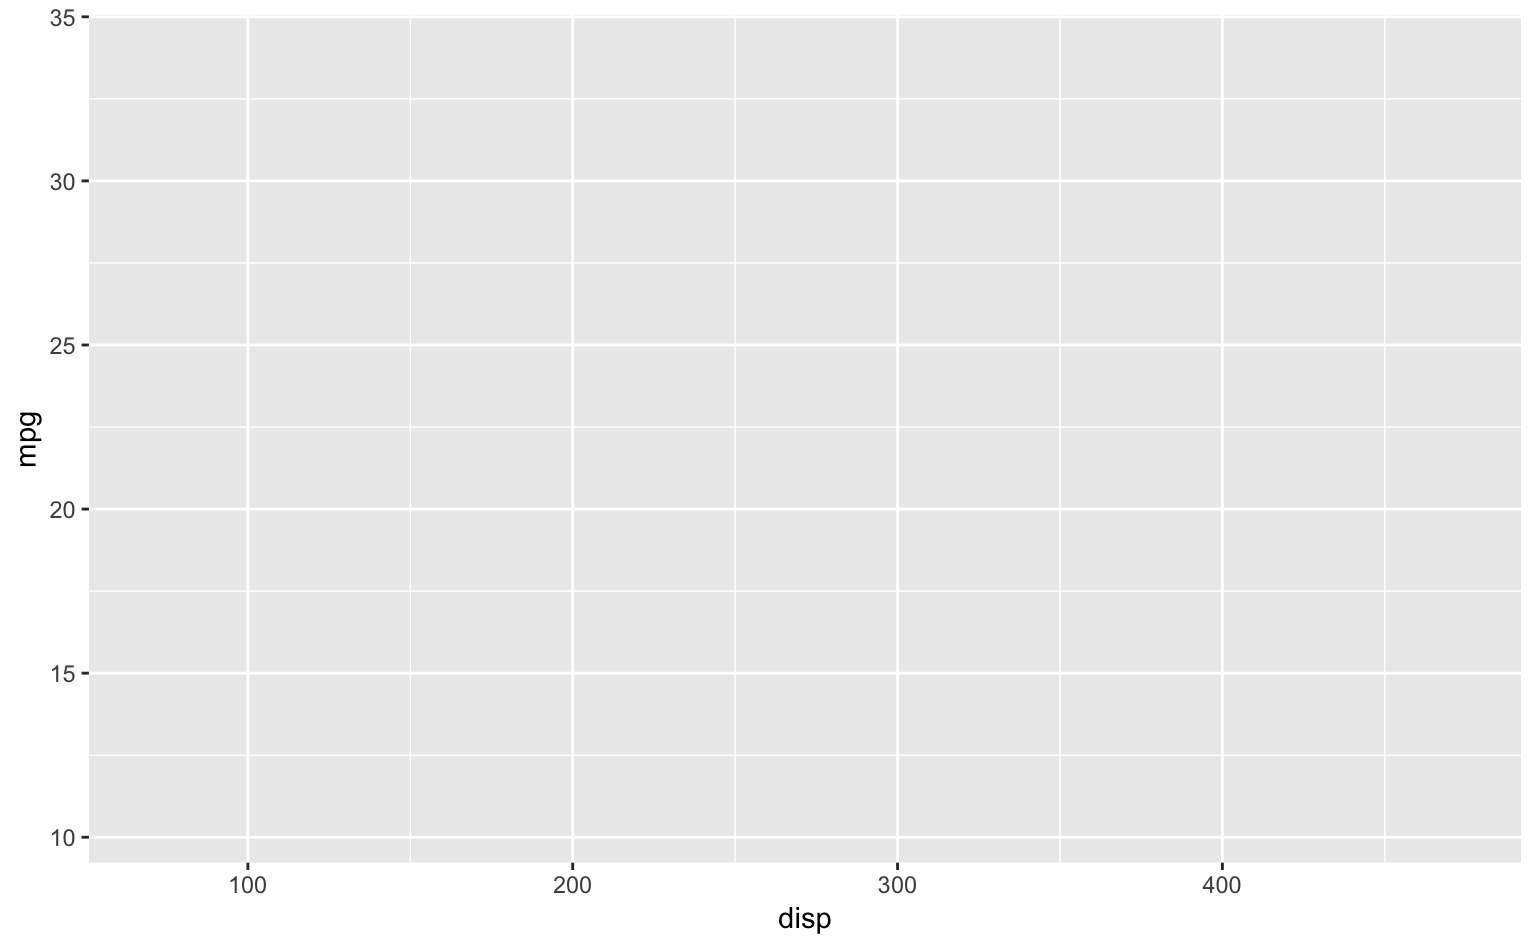
\includegraphics{lecture_note_files/figure-latex/unnamed-chunk-12-1} 

}

\caption{背景のみのグラフ。}\label{fig:unnamed-chunk-12}
\end{figure}

しかし、灰色の背景があるだけでデータはプロットされない。なぜなら、どのようなデザイン\footnote{ggplot2において厳密にはレイヤー(layer)などと呼んだりするが、そこら辺は入門段階ではあまり気にしなくて良い。というか、ぶっちゃけ筆者自身も厳密なことはわかっていない。}でデータをプロットするかを指示していないからである。つまり、これだけではまだ足りない。

\textbf{2. どのようなデザインでプロットしたいかを指示する}

データをどのようなデザイン(geometry)でプロットしたいかを、\texttt{geom\_xxxx()}で指定しなければならない。今回は散布図(データを点としてプロット)なので、\texttt{geom\_point()}というコードを使う。

先程のコードに「+」でコードをつなげていくことでプロットできるようになる。



\begin{Shaded}
\begin{Highlighting}[]
\KeywordTok{ggplot}\NormalTok{(}\DataTypeTok{data =}\NormalTok{ mtcars, }\KeywordTok{aes}\NormalTok{(}\DataTypeTok{x =}\NormalTok{ disp, }\DataTypeTok{y =}\NormalTok{ mpg)) }\OperatorTok{+}\StringTok{ }\CommentTok{# コードを読みやすくするため、「+」のところで改行すると良い}
\StringTok{  }\KeywordTok{geom_point}\NormalTok{() }\CommentTok{# データを点(point)としてデザインするためのコードを追加}
\end{Highlighting}
\end{Shaded}

\begin{figure}

{\centering 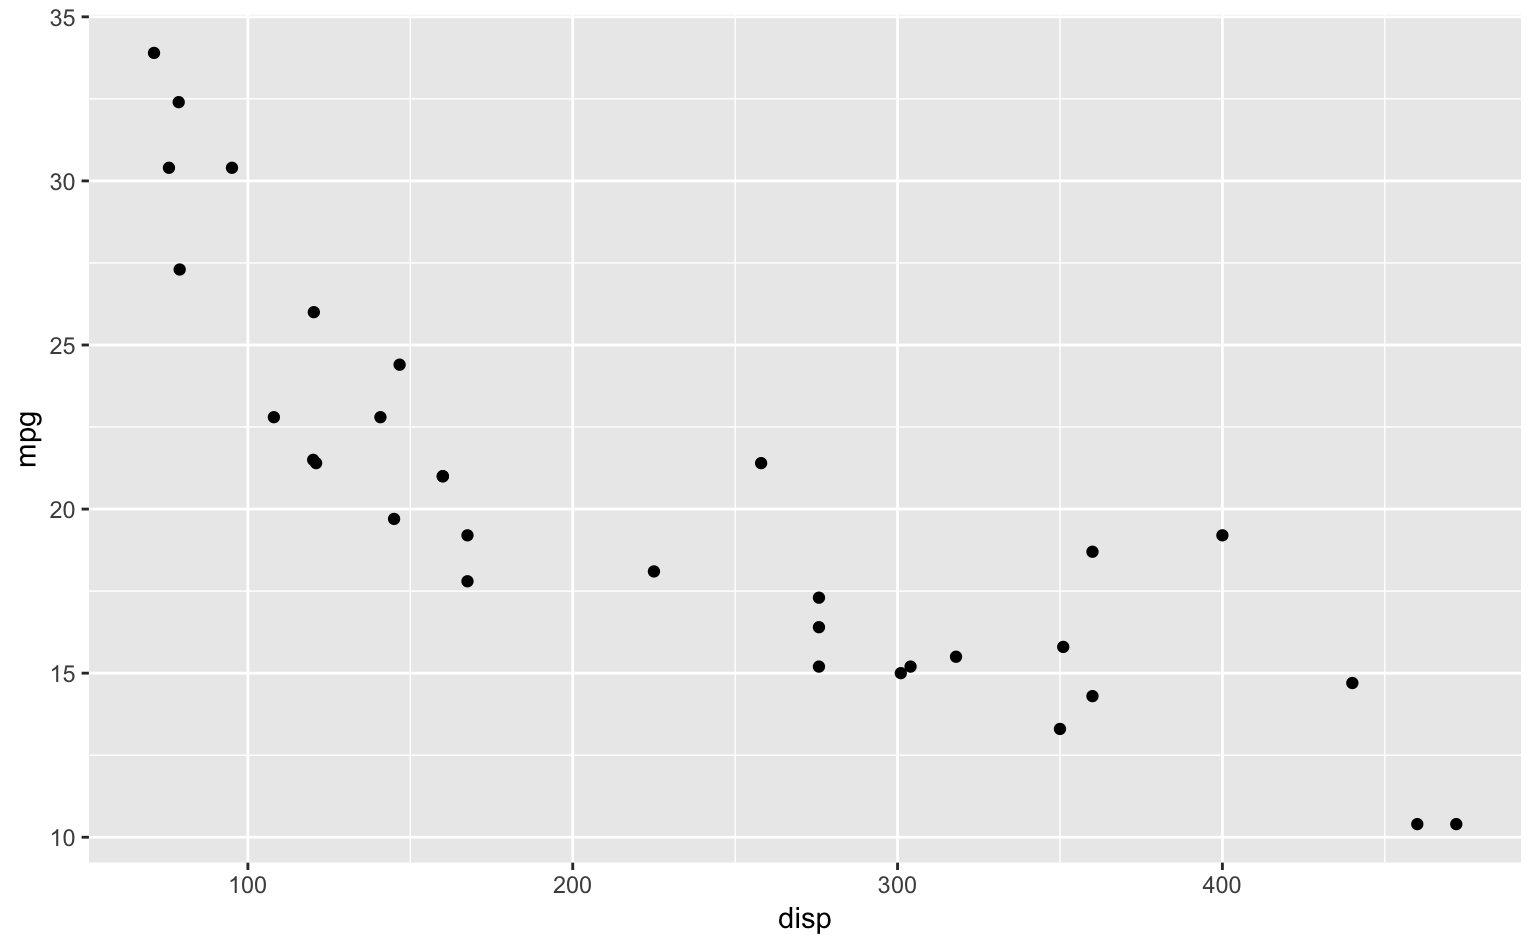
\includegraphics{lecture_note_files/figure-latex/tutorial-2-1} 

}

\caption{散布図。x軸は排気量、y軸は燃費を表している。}\label{fig:tutorial-2}
\end{figure}

完成。基本はこれだけである。

なお、ほとんどのグラフはx軸とy軸から構成されるので、実はコードの中に一々\texttt{x\ =\ disp}や\texttt{y\ =\ mpg}と書く必要はない。また、データについても自明なので、\texttt{data\ =\ mtcars}と書く必要もない。つまり、上のコードは下のように書くこともできる(これ以降、data,
x, yは省略する)。




\begin{Shaded}
\begin{Highlighting}[]
\KeywordTok{ggplot}\NormalTok{(mtcars, }\KeywordTok{aes}\NormalTok{(disp, mpg)) }\OperatorTok{+}
\StringTok{  }\KeywordTok{geom_point}\NormalTok{()}
\end{Highlighting}
\end{Shaded}

\begin{figure}

{\centering 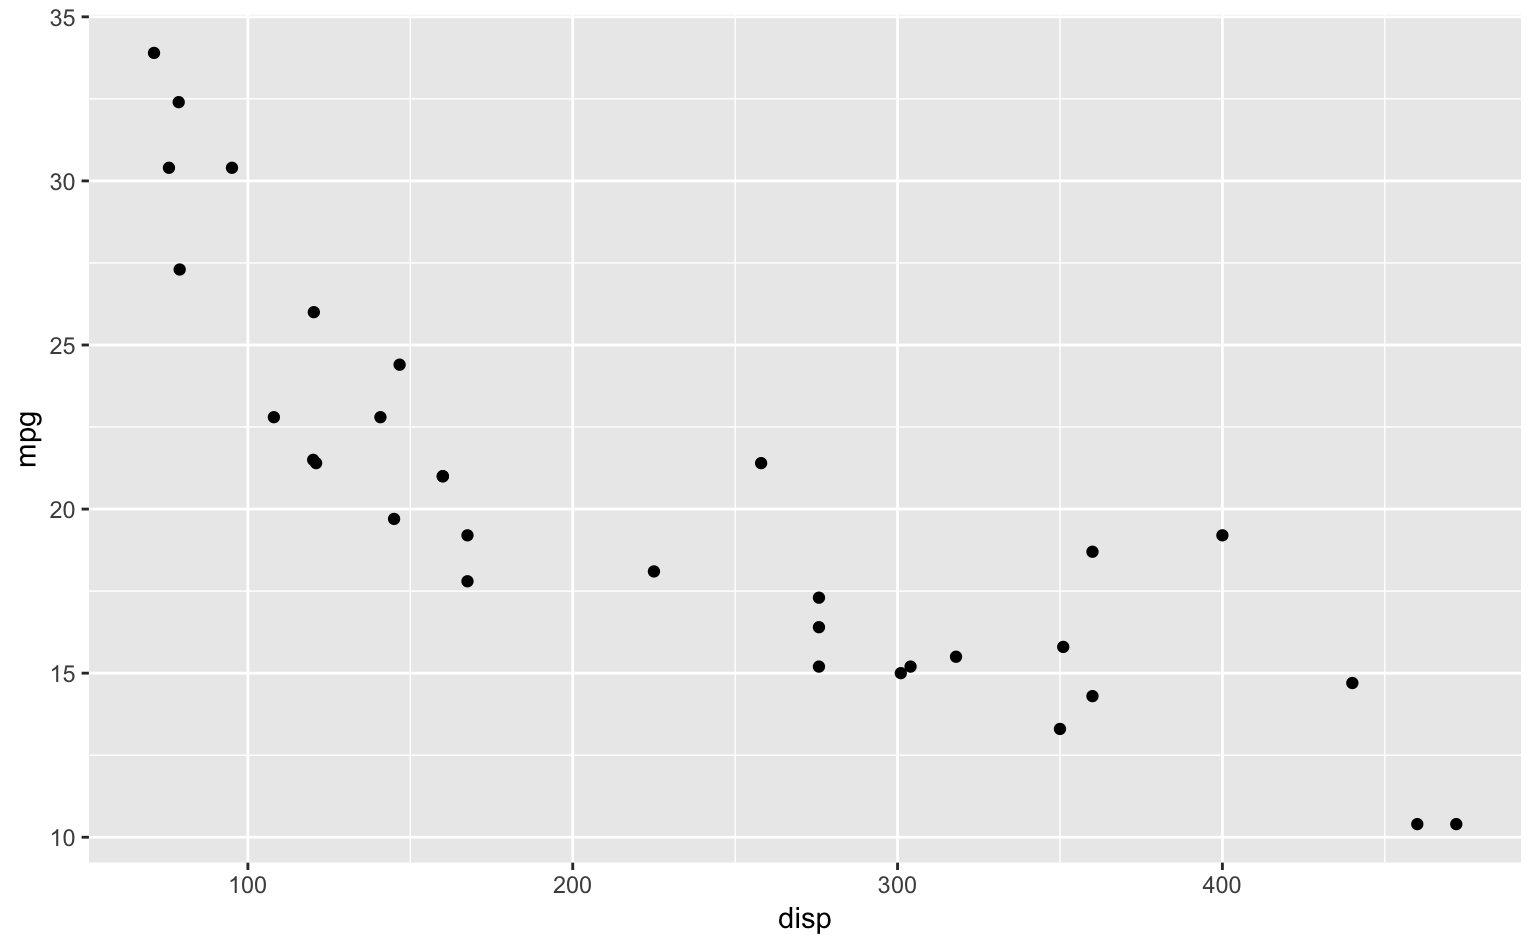
\includegraphics{lecture_note_files/figure-latex/unnamed-chunk-13-1} 

}

\caption{コードは若干違うが、上のFigure
\ref{fig:tutorial-2}と全く同じ散布図。}\label{fig:unnamed-chunk-13}
\end{figure}

\textbf{3. 変数を色(や形状)に対応づける}

もちろん上の図ができた時点でOKだが、これだけではどうも味気ない。では、ここで一歩進んで、もう1つ変数を加えてみよう。その変数とは、

\begin{itemize}
\tightlist
\item
  \texttt{cyl}:シリンダーの個数(4, 6, or 8)
\end{itemize}

である。このとき「シリンダーの個数によって、排気量と燃費の関係は違うのではないか?」ということが思いつく。

それでは、\texttt{cyl}によって点の色を変えてみよう。以下のコードを書けばOKである。



\begin{Shaded}
\begin{Highlighting}[]
\KeywordTok{ggplot}\NormalTok{(mtcars, }\KeywordTok{aes}\NormalTok{(disp, mpg, }\DataTypeTok{color =}\NormalTok{ cyl)) }\OperatorTok{+}\StringTok{ }\CommentTok{# color = cyl を追加}
\StringTok{  }\KeywordTok{geom_point}\NormalTok{()}
\end{Highlighting}
\end{Shaded}

\begin{figure}

{\centering 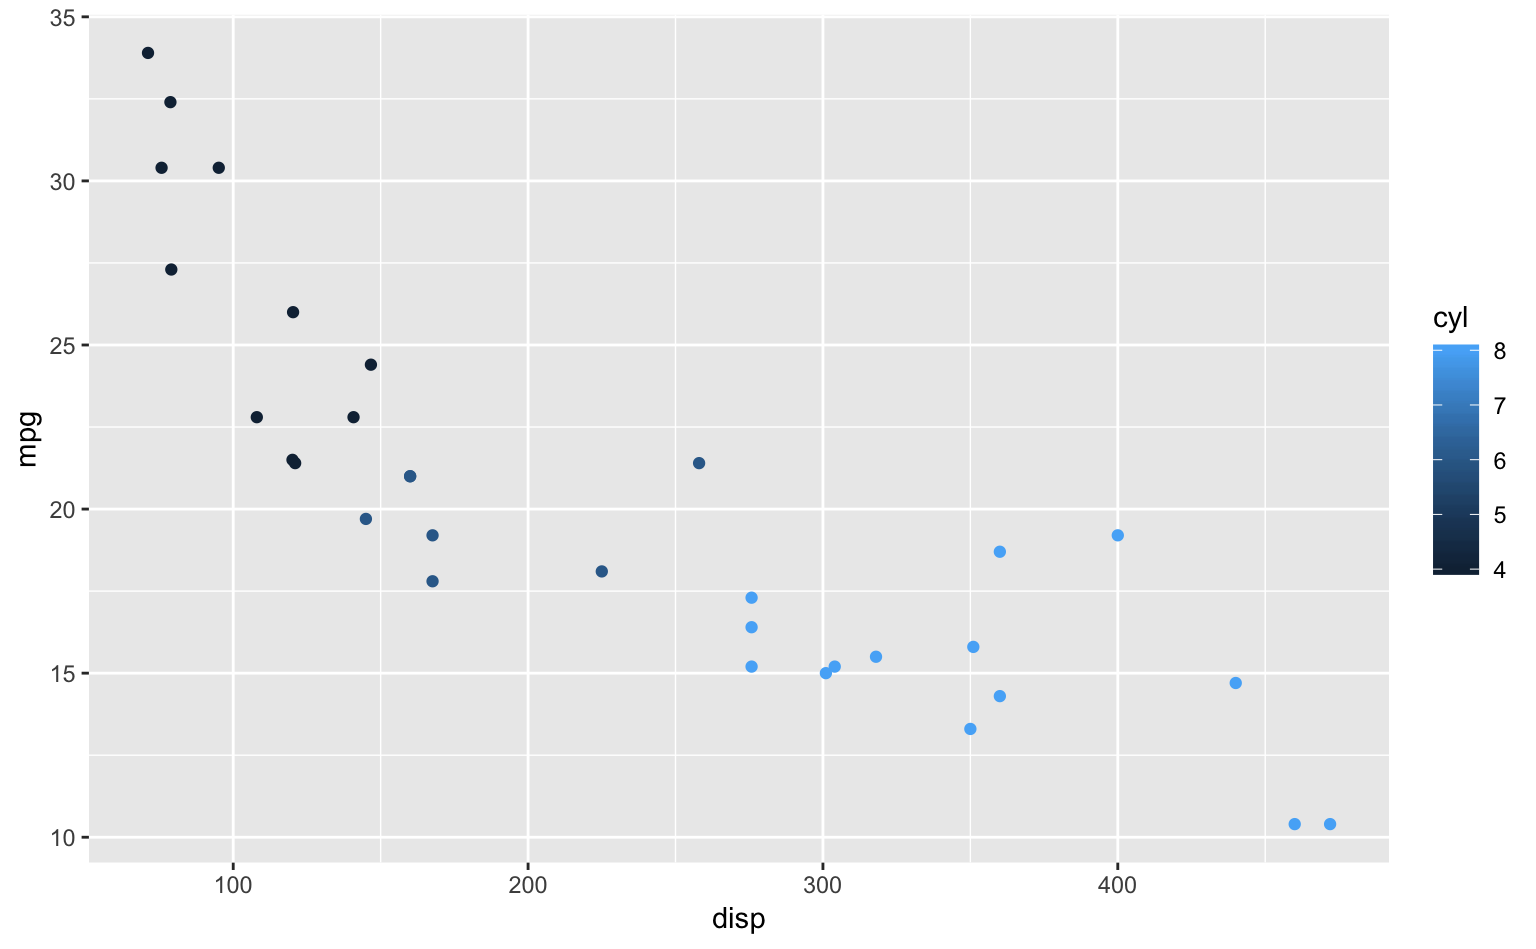
\includegraphics{lecture_note_files/figure-latex/unnamed-chunk-14-1} 

}

\caption{シリンダーの個数を点の色に対応づけた散布図。}\label{fig:unnamed-chunk-14}
\end{figure}

\texttt{aes()}に\texttt{color\ =\ cyl}を追加することで、\texttt{cyl}を色に対応づけることができた。

\textbf{しかし、このグラフは厳密には間違っている。}どこが間違っているのだろうか? 少し考えてみてほしい。

\textbf{答え}

図の右側の青いバー(\textbf{凡例};legend)を見ると、その横にシリンダーの個数が連続変数として1刻みで描かれれている(4,5,6,7,8)。しかし、実際のデータには4,6,8という3種類の値しかない。もちろん個数は連続的なものだが、この場合は\textbf{離散変数}(discrete
variable;質的変数、qualitative/categorical/factor
variableとも言う)として扱ったほうがデータの表現として妥当だし、見やすくなるだろう\footnote{変数が連続か離散かという区別は、可視化の上で結構重要なので意識しておくと良い。}。

この場合、\texttt{cyl}を\texttt{factor()}でくくると解決する。



\begin{Shaded}
\begin{Highlighting}[]
\KeywordTok{ggplot}\NormalTok{(mtcars, }\KeywordTok{aes}\NormalTok{(disp, mpg, }\DataTypeTok{color =} \KeywordTok{factor}\NormalTok{(cyl))) }\OperatorTok{+}\StringTok{ }\CommentTok{# factor(cyl)に変更}
\StringTok{  }\KeywordTok{geom_point}\NormalTok{()}
\end{Highlighting}
\end{Shaded}

\begin{figure}

{\centering 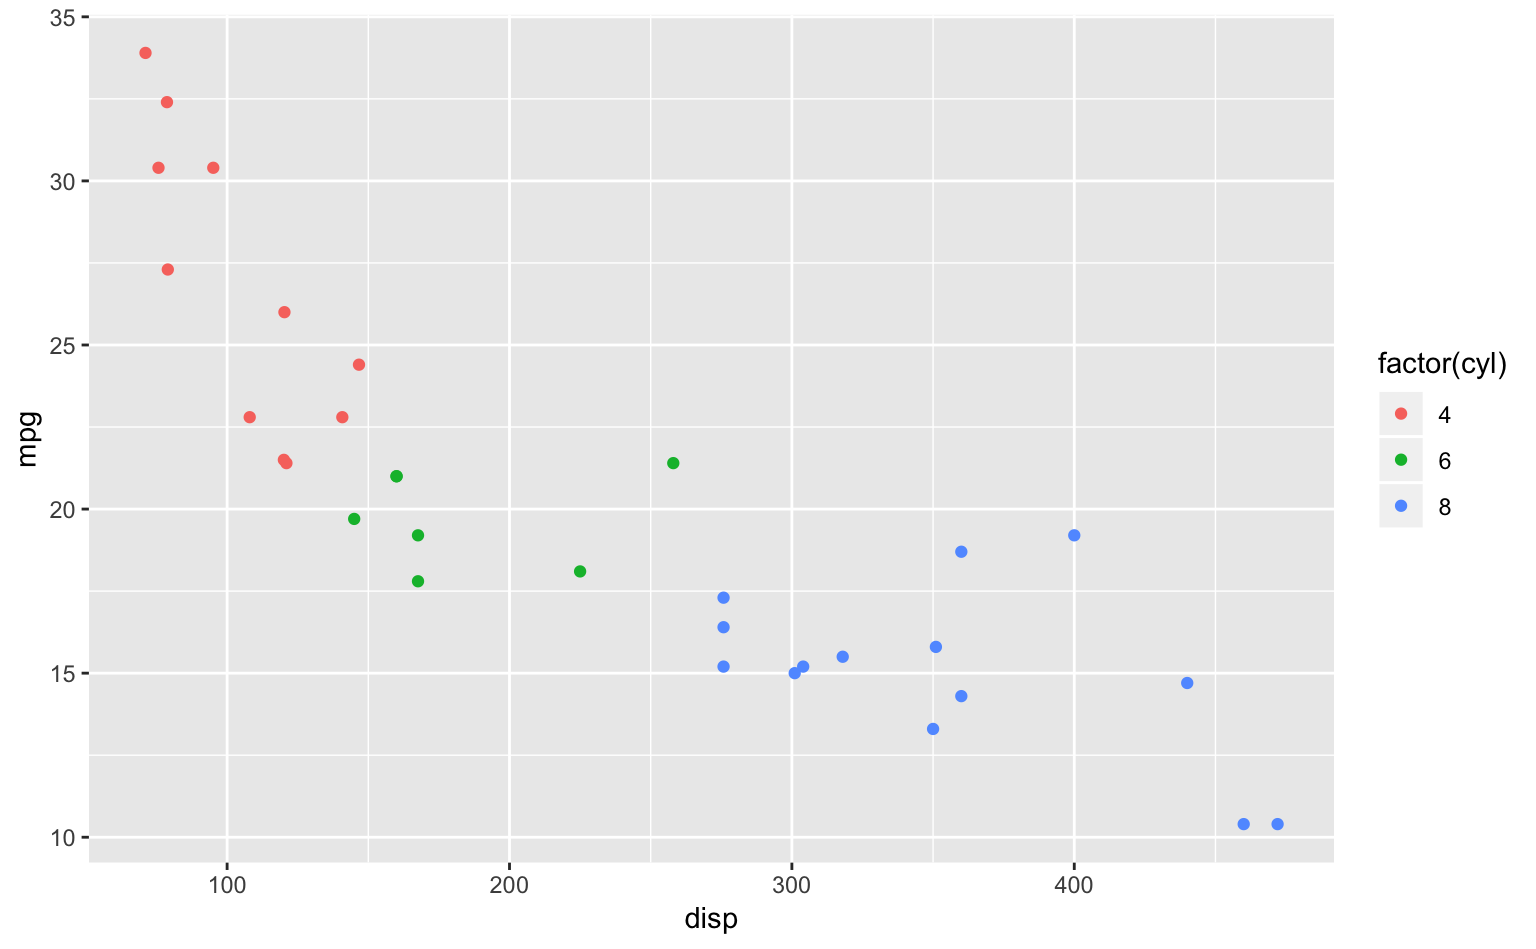
\includegraphics{lecture_note_files/figure-latex/tutorial-5-1} 

}

\caption{シリンダー数を離散変数とした上で色に対応づけた散布図。}\label{fig:tutorial-5}
\end{figure}

Rでは、\texttt{factor(変数)}とすることで、その変数を離散変数として扱うことができるようになる。その結果、凡例の表示も妥当なものとなった。

\section{まとめ}

このように、ggplot2を使うと、数行のコードでそれなりに見栄えの良い図が描けるようになる。

手順をもう一度おさらいしよう。

\textbf{1. x軸とy軸にどの変数を対応づけたいかを考える}

\begin{itemize}
\item
  \textbf{何(y軸)を何(x軸)に応じてプロットしたいかを考えるのが可視化の第一歩である。}
\item
  これが思いつけば可視化は大体うまくいったようなものである。
\end{itemize}

\textbf{2. どのようなデザインでプロットしたいかを指示する}

\begin{itemize}
\item
  \textbf{データの性質(特に離散変数か連続変数か)に応じてデザインを決める。}
\item
  たとえば「x軸が連続変数でy軸が連続変数なら散布図」というように決める。こういうのは大体コンセンサスが取れている\footnote{これはヒューリスティックであり、時には例外もある。しかし、大体の場合正しい。}ので、以降の章でそれを学んでいってほしい。
\item
  今回は散布図しか描かなかったが、たとえば散布図の上に回帰直線を重ね書きする、というように、複数の表現を組み合わせてプロットすることも可能である。これは追々見ていくことにする。
\end{itemize}

\textbf{3. 変数を色(や形状)に対応づける}

\begin{itemize}
\item
  \textbf{x軸、y軸以外に追加したい変数がある場合は、色などに対応づける。}
\item
  まずは基本のプロットができるようになることを目指すので、細かい色の調整方法などは後の方で少しだけ解説する。
\end{itemize}

\begin{center}\rule{0.5\linewidth}{\linethickness}\end{center}

下に載せているのはあくまでごく一部だが、ggplot2では以下のデザイン(\texttt{geom\_xxxx()})を使うことが多い。

\begin{longtable}[]{@{}ll@{}}
\toprule
geom & デザイン\tabularnewline
\midrule
\endhead
geom\_bar() & 棒グラフ\tabularnewline
geom\_line() & 折れ線グラフ\tabularnewline
geom\_point() & 散布図、点\tabularnewline
geom\_errorbar() & エラーバー\tabularnewline
geom\_pointrange() & 点+線\tabularnewline
geom\_histogram() & ヒストグラム\tabularnewline
geom\_density() & 密度曲線\tabularnewline
geom\_boxplot() & 箱ひげ図\tabularnewline
geom\_violin() & バイオリンプロット\tabularnewline
geom\_area() & 面グラフ\tabularnewline
geom\_smooth() & 関数のフィッティング\tabularnewline
geom\_text() & テキスト\tabularnewline
\bottomrule
\end{longtable}

これもまたごく一部だが、変数は\texttt{x}、\texttt{y}、\texttt{color}だけでなく、以下の要素(\texttt{aes()})にも対応づけることができる。

\begin{longtable}[]{@{}ll@{}}
\toprule
aes() & 要素\tabularnewline
\midrule
\endhead
x & x軸\tabularnewline
y & y軸\tabularnewline
color & 枠の色\tabularnewline
fill & 塗りつぶしの色\tabularnewline
linetype & 線の形\tabularnewline
size & 線の太さ、点の大きさ\tabularnewline
shape & 点の形\tabularnewline
\bottomrule
\end{longtable}

以降の章では、よく用いる可視化のパターンについて見ていくことにする。

\chapter{数量}\label{amount}

基本中の基本として、まずはデータの数量(数値、個数、比率、順位など)を可視化してみよう。

\begin{Shaded}
\begin{Highlighting}[]
\KeywordTok{library}\NormalTok{(ggplot2) }\CommentTok{# 忘れずにパッケージを読み込む}
\end{Highlighting}
\end{Shaded}

\section{棒グラフ}

\subsection{基本の棒グラフ}

数量の可視化で最も代表的、かつ馴染み深いのは\textbf{棒グラフ}(bar
graph; bar chart; bar plot)だろう。

まず、最も基本的な棒グラフを描いてみよう。使うデータは、gcookbookパッケージの\texttt{pg\_mean}(植物の重さに関するデータセット)である。まず、gcookbookを読み込む。

\begin{Shaded}
\begin{Highlighting}[]
\KeywordTok{library}\NormalTok{(gcookbook)}
\end{Highlighting}
\end{Shaded}

データの中身は以下の通りである。

\begin{Shaded}
\begin{Highlighting}[]
\KeywordTok{head}\NormalTok{(pg_mean) }\CommentTok{# データが3行しかないのですべて表示される}
\end{Highlighting}
\end{Shaded}

\begin{verbatim}
##   group weight
## 1  ctrl  5.032
## 2  trt1  4.661
## 3  trt2  5.526
\end{verbatim}

2つの変数はそれぞれ

\begin{itemize}
\item
  \texttt{group}:実験の条件(3水準)
\item
  \texttt{weight}:植物の重さの平均値
\end{itemize}

を表している。素朴に思いつくのは、「条件をx軸に、重さをy軸に取った棒グラフ」だろう。数量を表す棒グラフは、\texttt{geom\_bar()}で描くことができる。



\begin{Shaded}
\begin{Highlighting}[]
\KeywordTok{ggplot}\NormalTok{(pg_mean, }\KeywordTok{aes}\NormalTok{(group, weight)) }\OperatorTok{+}\StringTok{ }\CommentTok{# x軸にgroup、y軸にweight}
\StringTok{  }\KeywordTok{geom_bar}\NormalTok{(}\DataTypeTok{stat =} \StringTok{"identity"}\NormalTok{) }\CommentTok{# 棒グラフ;stat = "identity"が必要}
\end{Highlighting}
\end{Shaded}

\begin{figure}

{\centering 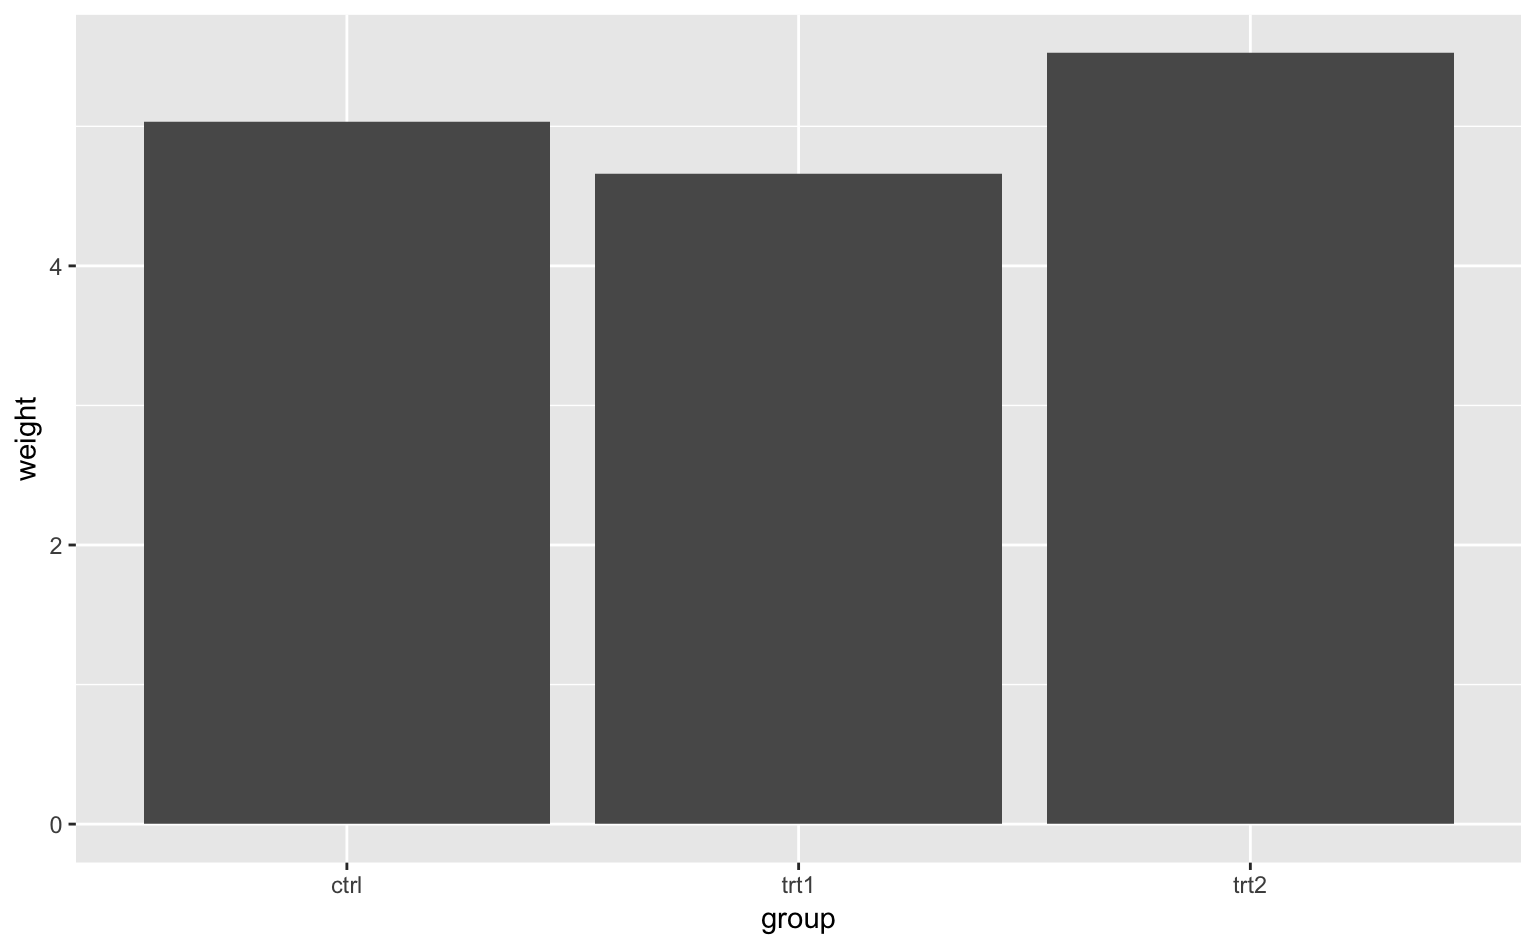
\includegraphics{lecture_note_files/figure-latex/unnamed-chunk-19-1} 

}

\caption{棒グラフ。x軸は条件、y軸は植物の平均重量を表している。}\label{fig:unnamed-chunk-19}
\end{figure}

なお、データの数値を棒グラフで描く際は、\texttt{stat\ =\ "identity"}と設定する必要がある。なぜなら、\texttt{geom\_bar()}は、データの\textbf{個数}を描くのがデフォルト(\texttt{stat\ =\ "count"}という設定)になっているからである\footnote{ここら辺のことはいずれわかるようになるので、今はそういうものだと飲み込んでほしい。いずれ勝手に理解できているはず(たぶん)。}。

気になる人は、\texttt{stat\ =\ "identity"}の部分を消してコードを実行してみよう。\texttt{エラー:\ stat\_count()\ must\ not\ be\ used\ with\ a\ y\ aesthetic.}というメッセージが出てきて、プロットできないはずである\footnote{本資料のコードを修正した上で実行してもPCが壊れたりすることはないので、「ここをこうしたらどうなるだろうか?」と積極的にいじってみることを推奨する。}。

\subsection{グルーピングされた棒グラフ}

では、ここに変数を1つ追加してみよう。次に使うデータはgcookbookの\texttt{cabbage\_exp}(キャベツに関するデータセット)である。

\begin{Shaded}
\begin{Highlighting}[]
\KeywordTok{head}\NormalTok{(cabbage_exp) }\CommentTok{# 6行しかないのですべて表示される}
\end{Highlighting}
\end{Shaded}

\begin{verbatim}
##   Cultivar Date Weight        sd  n         se
## 1      c39  d16   3.18 0.9566144 10 0.30250803
## 2      c39  d20   2.80 0.2788867 10 0.08819171
## 3      c39  d21   2.74 0.9834181 10 0.31098410
## 4      c52  d16   2.26 0.4452215 10 0.14079141
## 5      c52  d20   3.11 0.7908505 10 0.25008887
## 6      c52  d21   1.47 0.2110819 10 0.06674995
\end{verbatim}

注目する変数は以下の3つである。

\begin{itemize}
\item
  \texttt{Date}:キャベツの栽培期間(d16, d20, or d21)
\item
  \texttt{Cultivar}:キャベツの品種(c39 or c52)
\item
  \texttt{Weight}:キャベツの重量(kg)
\end{itemize}

このとき、栽培期間と品種ごとにキャベツの重量を描いてみたいと思わない人はいない\footnote{異論は認めない。}。このようなときは、\texttt{Date}を\texttt{x}、\texttt{Weight}を\texttt{y}、\texttt{Cultivar}を\texttt{fill}に対応づけて描けば良い。



\begin{Shaded}
\begin{Highlighting}[]
\KeywordTok{ggplot}\NormalTok{(cabbage_exp, }\KeywordTok{aes}\NormalTok{(Date, Weight, }\DataTypeTok{fill =}\NormalTok{ Cultivar)) }\OperatorTok{+}\StringTok{ }\CommentTok{# x軸にDate、y軸にWeight;fill = Cultivarを追加}
\StringTok{  }\KeywordTok{geom_bar}\NormalTok{(}\DataTypeTok{stat =} \StringTok{"identity"}\NormalTok{, }\DataTypeTok{position =} \StringTok{"dodge"}\NormalTok{) }\CommentTok{# 棒グラフ;position = "dodge"が必要}
\end{Highlighting}
\end{Shaded}

\begin{figure}

{\centering 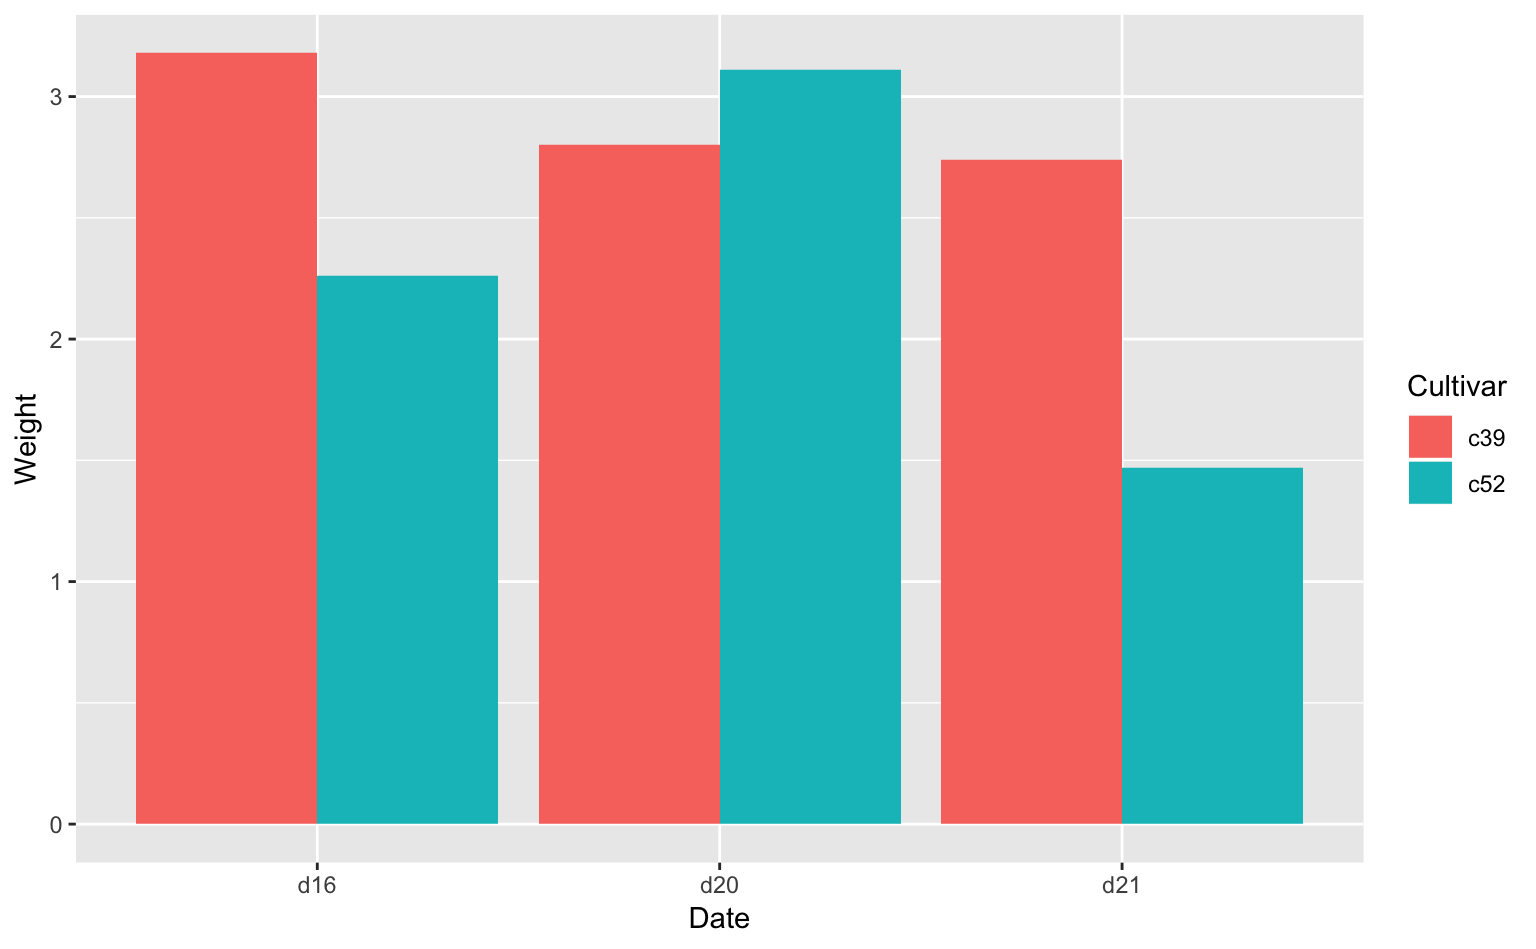
\includegraphics{lecture_note_files/figure-latex/bar-plot-2-1} 

}

\caption{グルーピングされた棒グラフ。}\label{fig:bar-plot-2}
\end{figure}

このように、2つの変数ごとに棒グラフを描きたい(グルーピングしたい)場合は、\texttt{fill}に変数を追加すれば良い。\texttt{fill}は「塗りつぶし」を意味しており、実際\texttt{Cultivar}の種類に応じて棒が塗りつぶされていることがわかる\footnote{「色なのだから、\texttt{color}に変数を指定するのでは?」と思った人がいるかもしれない。実際、\texttt{geom\_bar()}で\texttt{color}に変数を指定すると、棒の\textbf{枠線の色}が変わる。しかし、棒グラフの枠に色をつけてもごちゃごちゃするだけなので、基本的には変数を指定する必要はない。}。

なお、このようなグラフを描く際は、基本的に\texttt{position\ =\ "dodge"}と指定する必要がある。なぜなら、\texttt{geom\_bar()}はデフォルトが\texttt{position\ =\ "stack"}であり、そのままだと積み上げ棒グラフになってしまうからである。ちなみに、\texttt{position\ =\ "fill"}と指定すれば、全体を100\%にした積み上げ棒グラフを描くことができる。積み上げ棒グラフは割合や比率を表すのによく使われるグラフである。

\subsection{個数を表す棒グラフ}

では、データの数値ではなく、データの\textbf{個数}(カウントデータ)はどのようにプロットすればよいだろうか? 次は、ggplot2の\texttt{diamonds}(ダイアモンドに関するデータセット)を使ってみよう。

\begin{Shaded}
\begin{Highlighting}[]
\KeywordTok{head}\NormalTok{(diamonds) }\CommentTok{# 先頭6行}
\end{Highlighting}
\end{Shaded}

\begin{verbatim}
## # A tibble: 6 x 10
##   carat cut       color clarity depth table price     x     y     z
##   <dbl> <ord>     <ord> <ord>   <dbl> <dbl> <int> <dbl> <dbl> <dbl>
## 1 0.23  Ideal     E     SI2      61.5    55   326  3.95  3.98  2.43
## 2 0.21  Premium   E     SI1      59.8    61   326  3.89  3.84  2.31
## 3 0.23  Good      E     VS1      56.9    65   327  4.05  4.07  2.31
## 4 0.290 Premium   I     VS2      62.4    58   334  4.2   4.23  2.63
## 5 0.31  Good      J     SI2      63.3    58   335  4.34  4.35  2.75
## 6 0.24  Very Good J     VVS2     62.8    57   336  3.94  3.96  2.48
\end{verbatim}

ここでは\texttt{cut}という変数に着目してみよう。

\begin{itemize}
\tightlist
\item
  \texttt{cut}:ダイアモンドのカットの質(Fair, Good, Very Good,
  Premium, or Ideal)
\end{itemize}

ダイアモンドの個数をカットに応じてプロットしてみよう。なお、\texttt{geom\_bar()}はデータの個数を自動的に数えてくれるので、\texttt{y}に変数を対応づける必要はない。



\begin{Shaded}
\begin{Highlighting}[]
\KeywordTok{ggplot}\NormalTok{(diamonds, }\KeywordTok{aes}\NormalTok{(cut)) }\OperatorTok{+}\StringTok{ }\CommentTok{# x軸にcut;yには何も対応づける必要なし}
\StringTok{  }\KeywordTok{geom_bar}\NormalTok{() }\CommentTok{# 棒グラフ;今回はデータの値ではなく個数を描くので、stat = "identity"は不要}
\end{Highlighting}
\end{Shaded}

\begin{figure}

{\centering 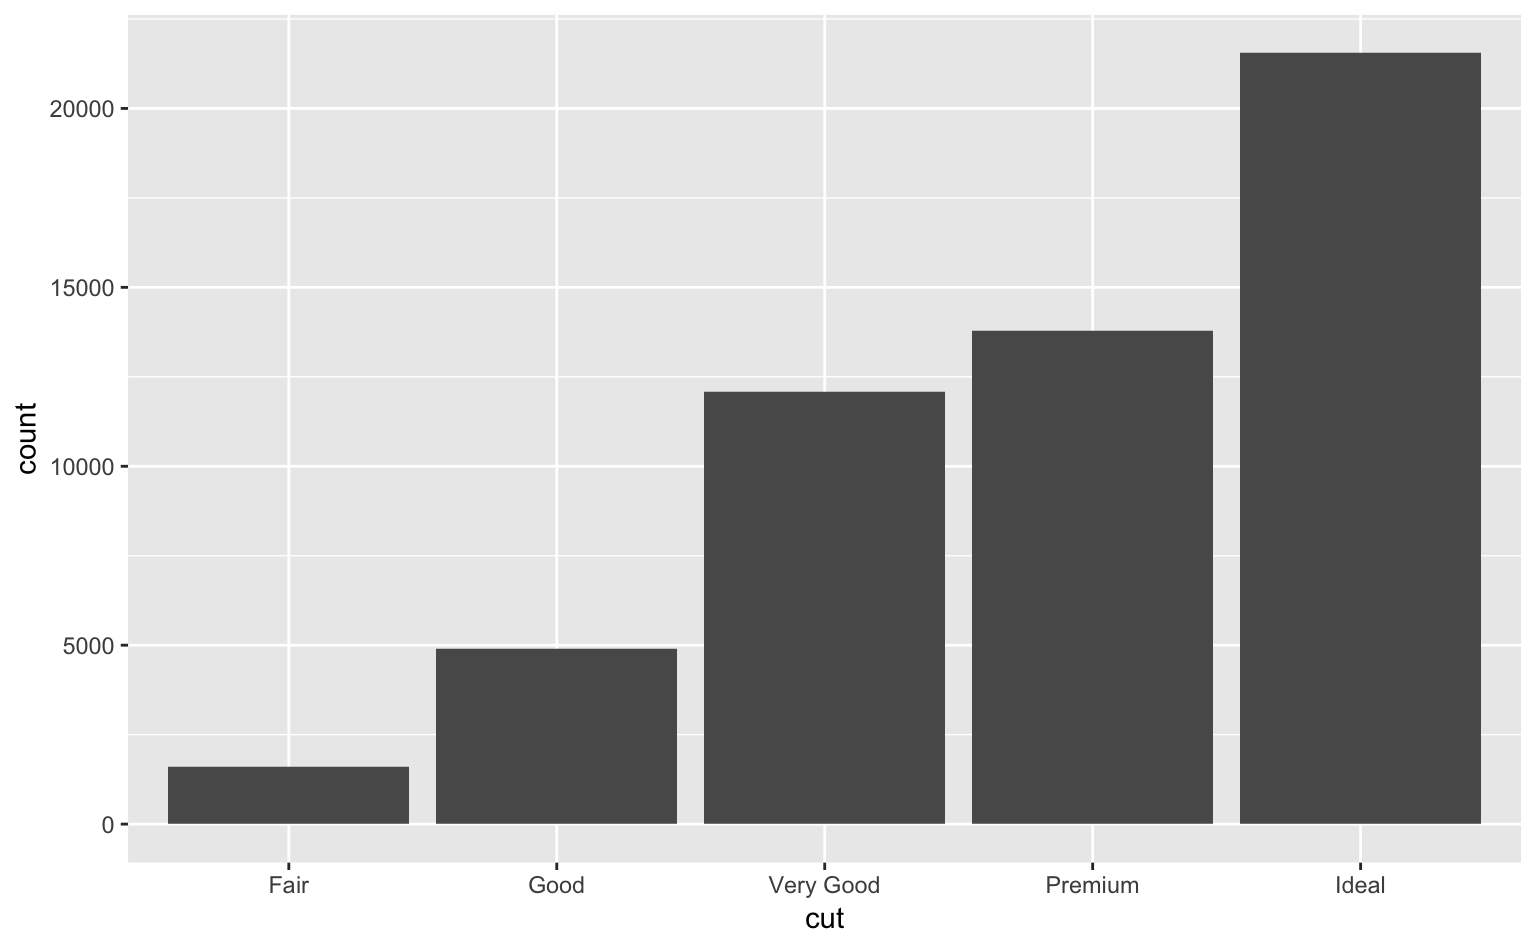
\includegraphics{lecture_note_files/figure-latex/bar-plot-3-1} 

}

\caption{カットごとのダイアモンドの個数。}\label{fig:bar-plot-3}
\end{figure}

無事に個数をプロットすることができた。

\section{Clevelandのドットプロット}\label{cleveland}

数量の可視化に向いているのは棒グラフだけではない。というよりもむしろ、棒グラフが可視化に向かない場合もある。たとえば、gcookbookの\texttt{tophitters2001}(2001年MLBの上位144打手のデータセット)を使ってそれを見てみよう。

\begin{Shaded}
\begin{Highlighting}[]
\KeywordTok{head}\NormalTok{(tophitters2001)}
\end{Highlighting}
\end{Shaded}

\begin{verbatim}
##          id   first   last           name year stint team lg   g  ab   r
## 1 walkela01   Larry Walker   Larry Walker 2001     1  COL NL 142 497 107
## 2 suzukic01  Ichiro Suzuki  Ichiro Suzuki 2001     1  SEA AL 157 692 127
## 3 giambja01   Jason Giambi   Jason Giambi 2001     1  OAK AL 154 520 109
## 4 alomaro01 Roberto Alomar Roberto Alomar 2001     1  CLE AL 157 575 113
## 5 heltoto01    Todd Helton    Todd Helton 2001     1  COL NL 159 587 132
## 6  aloumo01  Moises   Alou    Moises Alou 2001     1  HOU NL 136 513  79
##     h 2b 3b hr rbi sb cs  bb  so ibb hbp sh sf gidp    avg
## 1 174 35  3 38 123 14  5  82 103   6  14  0  8    9 0.3501
## 2 242 34  8  8  69 56 14  30  53  10   8  4  4    3 0.3497
## 3 178 47  2 38 120  2  0 129  83  24  13  0  9   17 0.3423
## 4 193 34 12 20 100 30  6  80  71   5   4  9  9    9 0.3357
## 5 197 54  2 49 146  7  5  98 104  15   5  1  5   14 0.3356
## 6 170 31  1 27 108  5  1  57  57  14   3  0  8   18 0.3314
\end{verbatim}

変数がたくさんあるが、とりあえず

\begin{itemize}
\item
  \texttt{name}:打手の名前
\item
  \texttt{avg}:打率
\end{itemize}

に注目してみよう。なお、データが144行と少し多いので、わかりやすさのため先頭の20名のデータだけを使うことにする。20名のデータは\texttt{top20hitters}に代入する。

\begin{Shaded}
\begin{Highlighting}[]
\NormalTok{top20hitters =}\StringTok{ }\NormalTok{tophitters2001[}\DecValTok{1}\OperatorTok{:}\DecValTok{20}\NormalTok{,] }\CommentTok{# 先頭20行を抽出してtop20hittersに代入}
\end{Highlighting}
\end{Shaded}

それでは、この\texttt{top20hitters}を使って、まずは打手ごとの打率を素直に棒グラフで描いてみよう。



\begin{Shaded}
\begin{Highlighting}[]
\KeywordTok{ggplot}\NormalTok{(top20hitters, }\KeywordTok{aes}\NormalTok{(name, avg)) }\OperatorTok{+}\StringTok{ }\CommentTok{# x軸にname、y軸にavg}
\StringTok{  }\KeywordTok{geom_bar}\NormalTok{(}\DataTypeTok{stat =} \StringTok{"identity"}\NormalTok{) }\CommentTok{# 棒グラフ}
\end{Highlighting}
\end{Shaded}

\begin{figure}

{\centering 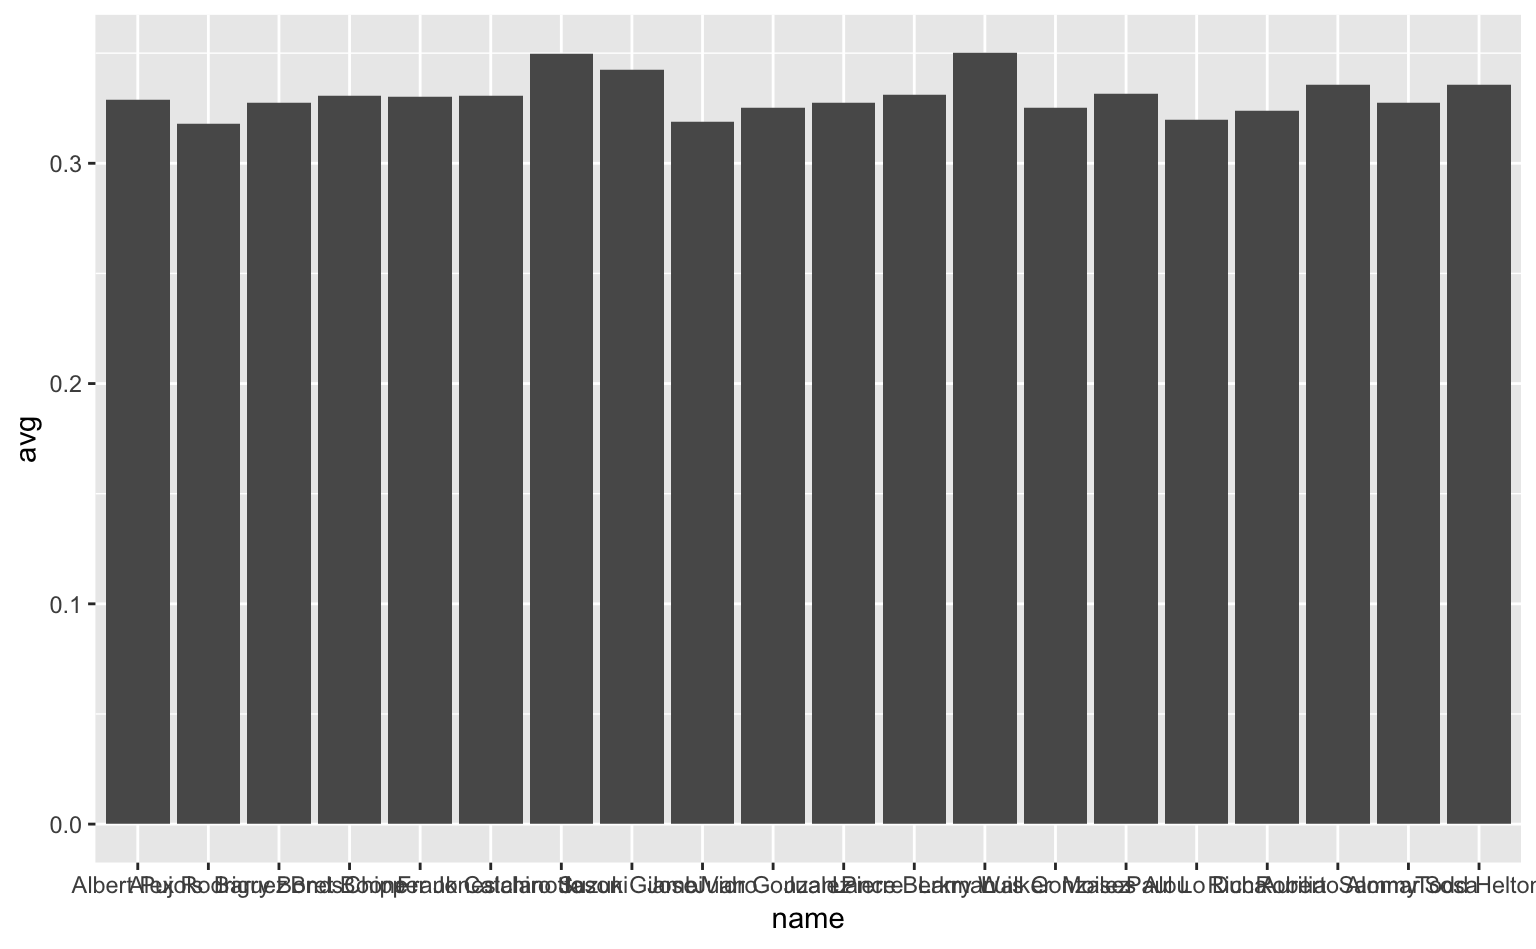
\includegraphics{lecture_note_files/figure-latex/bar-plot-4-1} 

}

\caption{2001年MLBのトップ20の打率。}\label{fig:bar-plot-4}
\end{figure}

これを見てどのように思うだろうか? おそらく「あまり美しくない」と感じる人が多いだろう。では、どこが問題なのか。大きく2つの問題点が挙げられるだろう。

\textbf{問題1. 選手ごとの打率の違いが明確に見えない}

\begin{itemize}
\tightlist
\item
  棒グラフはy = 0から始まるという性質がある\footnote{逆に、y =
    0から始まっていない棒グラフを見た場合、少し疑ってかかったほうが良い。このような棒グラフは結構巷にあふれている。}。しかし、今回のデータの値(打率)は基本的に0.3前後なので、y
  =
  0をグラフに含めるとデータの特徴が見えづらくなってしまう。このような場合、棒グラフは可視化に向いていない。
\end{itemize}

\textbf{問題2.
打率の高低によって選手が並び替えられていない(ソートされていない)}

\begin{itemize}
\tightlist
\item
  これは棒グラフ自体の問題ではないが、可視化において重要なポイントである。これも直す必要があるだろう。
\end{itemize}

\begin{center}\rule{0.5\linewidth}{\linethickness}\end{center}

これらの問題に対する解決策の1つとして、\textbf{Clevelandのドットプロット}(Cleveland
dot
plot)というものがある。ドットプロットというくらいなので、散布図のようにデータをドットで表現する手法である。描き方を順に見ていこう。



\begin{Shaded}
\begin{Highlighting}[]
\KeywordTok{ggplot}\NormalTok{(top20hitters, }\KeywordTok{aes}\NormalTok{(avg, }\KeywordTok{reorder}\NormalTok{(name, avg))) }\OperatorTok{+}\StringTok{ }\CommentTok{# x軸とy軸を交換、reorder()関数を使う}
\StringTok{  }\KeywordTok{geom_point}\NormalTok{() }\CommentTok{# ドットで描く;stat = "identity"は不要}
\end{Highlighting}
\end{Shaded}

\begin{figure}

{\centering 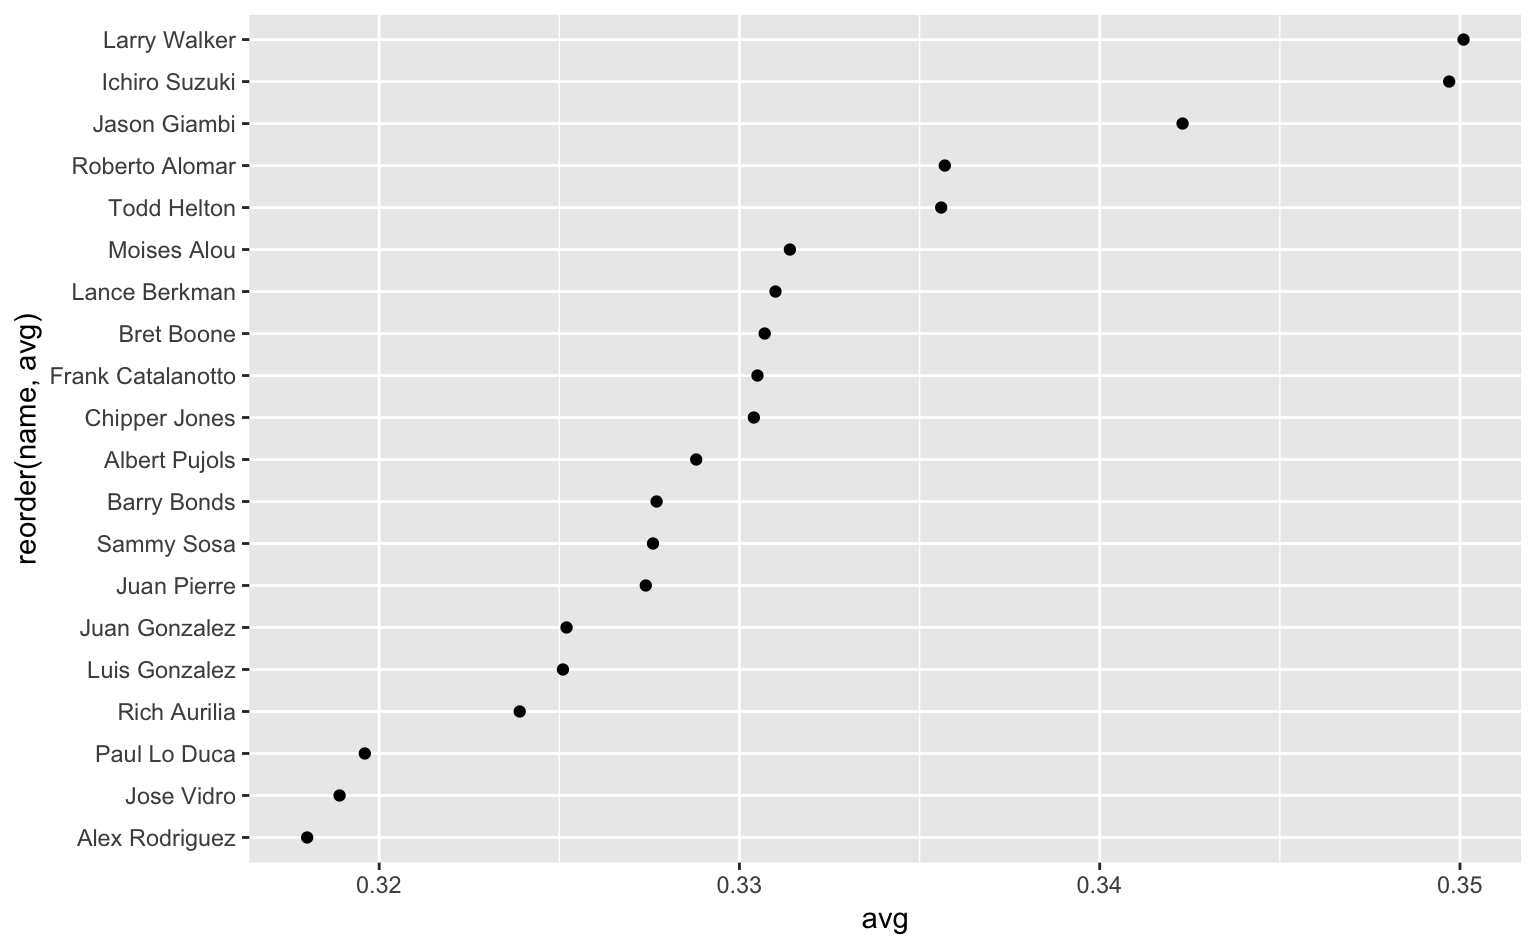
\includegraphics{lecture_note_files/figure-latex/dot-plot-1} 

}

\caption{Clevelandのドットプロット(2001年MLBトップ20の打率)。}\label{fig:dot-plot}
\end{figure}

\begin{enumerate}
\def\labelenumi{\arabic{enumi}.}
\item
  \texttt{ggplot(top20hitter,\ aes(avg,\ reorder(name,\ avg)))}

  \begin{itemize}
  \item
    打率をx軸、選手名をy軸にする。こうすることで、選手名が重ならずに済む。
  \item
    \texttt{reorder(name,\ avg)}により、選手名を打率でソートしている。\texttt{reorder(a,\ b)}はaをbの値で(昇順に)ソートする関数である。\texttt{reorder()}は、変数の\textbf{順序情報}を強調する際に使うと効果的である。
  \end{itemize}
\item
  \texttt{geom\_point()}

  \begin{itemize}
  \item
    データをドットで表現するための関数。
  \item
    ちなみに、\texttt{geom\_point()}では\texttt{stat\ =\ "identity"}がデフォルトである。そのため\texttt{geom\_bar()}とは異なり、\texttt{stat}の中身を明示的に指定する必要がない。
  \end{itemize}
\end{enumerate}

これがClevelandのドットプロット\footnote{類似のグラフとしてロリポッププロット(lollipop
  plot; lollipop
  chart)というものもある。\url{https://python-graph-gallery.com/lollipop-plot/}}である。改めてFigure
\ref{fig:bar-plot-4}とFigure
\ref{fig:dot-plot}を見比べると、明らかにグラフの見栄えが改善していることがわかる。

\section{練習問題}

\begin{itemize}
\item
  \texttt{cabbage\_exp}のデータを使い、x軸に\texttt{Cultivar}、y軸に\texttt{Weight}、\texttt{Date}で色分けした棒グラフを描いてみよう。
\item
  \texttt{diamonds}のデータを使い、\texttt{clarity}(輝きの等級)ごとにダイアモンドの個数をプロットしてみよう。
\item
  gcookbookの\texttt{uspopchange}のデータ構造を確認しよう(\texttt{?uspopchange}
  と
  \texttt{head(uspopchange)})。その上で、この章で学んだテクニックを使い、州ごとに人口がどれくらい増減したかをプロットしてみよう。また、どのようなデザインでプロットするのが最も妥当かつ見栄えが良いかを考えてみよう。
\end{itemize}

\chapter{分布}\label{distribution}

Chapter
\ref{introduction}の「アンスコムの例」で見たように、データの\textbf{要約統計量}(summary
statistics;記述統計量、descriptive
statisticsとも言う)だけに注目して、\textbf{分布}(distribution)を確認しないと痛い目にあうことがある。

\textbf{実験や調査でデータを集めたら、要約統計量を計算するだけでなく、まずデータの分布を確認・報告することを心がけよう。}

\begin{Shaded}
\begin{Highlighting}[]
\KeywordTok{library}\NormalTok{(ggplot2) }\CommentTok{# 忘れずにパッケージを読み込む}
\end{Highlighting}
\end{Shaded}

\section{ヒストグラム}

\subsection{基本のヒストグラム}

分布を表すグラフの中で最も代表的なのは\textbf{ヒストグラム}(histogram)だろう。ヒストグラムは複数の縦棒から構成されるグラフで、棒の幅(x軸)は変数の値、棒の高さ(y軸)はデータの個数を表している。

早速具体例を見てみよう。Chapter
\ref{introduction}と同様に、ここでもgcookbookの\texttt{tophitters2001}(2001年MLBにおける144名の打手データ)を使うことにする。gcookbookを読み込み、改めてデータ構造を再確認しよう。

\begin{Shaded}
\begin{Highlighting}[]
\KeywordTok{library}\NormalTok{(gcookbook)}
\end{Highlighting}
\end{Shaded}

\begin{Shaded}
\begin{Highlighting}[]
\KeywordTok{head}\NormalTok{(tophitters2001) }\CommentTok{# データの先頭6行を再確認}
\end{Highlighting}
\end{Shaded}

\begin{verbatim}
##          id   first   last           name year stint team lg   g  ab   r
## 1 walkela01   Larry Walker   Larry Walker 2001     1  COL NL 142 497 107
## 2 suzukic01  Ichiro Suzuki  Ichiro Suzuki 2001     1  SEA AL 157 692 127
## 3 giambja01   Jason Giambi   Jason Giambi 2001     1  OAK AL 154 520 109
## 4 alomaro01 Roberto Alomar Roberto Alomar 2001     1  CLE AL 157 575 113
## 5 heltoto01    Todd Helton    Todd Helton 2001     1  COL NL 159 587 132
## 6  aloumo01  Moises   Alou    Moises Alou 2001     1  HOU NL 136 513  79
##     h 2b 3b hr rbi sb cs  bb  so ibb hbp sh sf gidp    avg
## 1 174 35  3 38 123 14  5  82 103   6  14  0  8    9 0.3501
## 2 242 34  8  8  69 56 14  30  53  10   8  4  4    3 0.3497
## 3 178 47  2 38 120  2  0 129  83  24  13  0  9   17 0.3423
## 4 193 34 12 20 100 30  6  80  71   5   4  9  9    9 0.3357
## 5 197 54  2 49 146  7  5  98 104  15   5  1  5   14 0.3356
## 6 170 31  1 27 108  5  1  57  57  14   3  0  8   18 0.3314
\end{verbatim}

では、144名の打手の打率(\texttt{avg})の分布を可視化してみよう。ヒストグラムはx軸に連続変数の値を取るグラフなので、以下のようにコードを書けば良い。



\begin{Shaded}
\begin{Highlighting}[]
\KeywordTok{ggplot}\NormalTok{(tophitters2001, }\KeywordTok{aes}\NormalTok{(avg)) }\OperatorTok{+}\StringTok{ }\CommentTok{# x軸にavg;データの個数は自動的にカウントされるので、yは指定する必要なし}
\StringTok{  }\KeywordTok{geom_histogram}\NormalTok{() }\CommentTok{# ヒストグラムを描く}
\end{Highlighting}
\end{Shaded}

\begin{figure}

{\centering 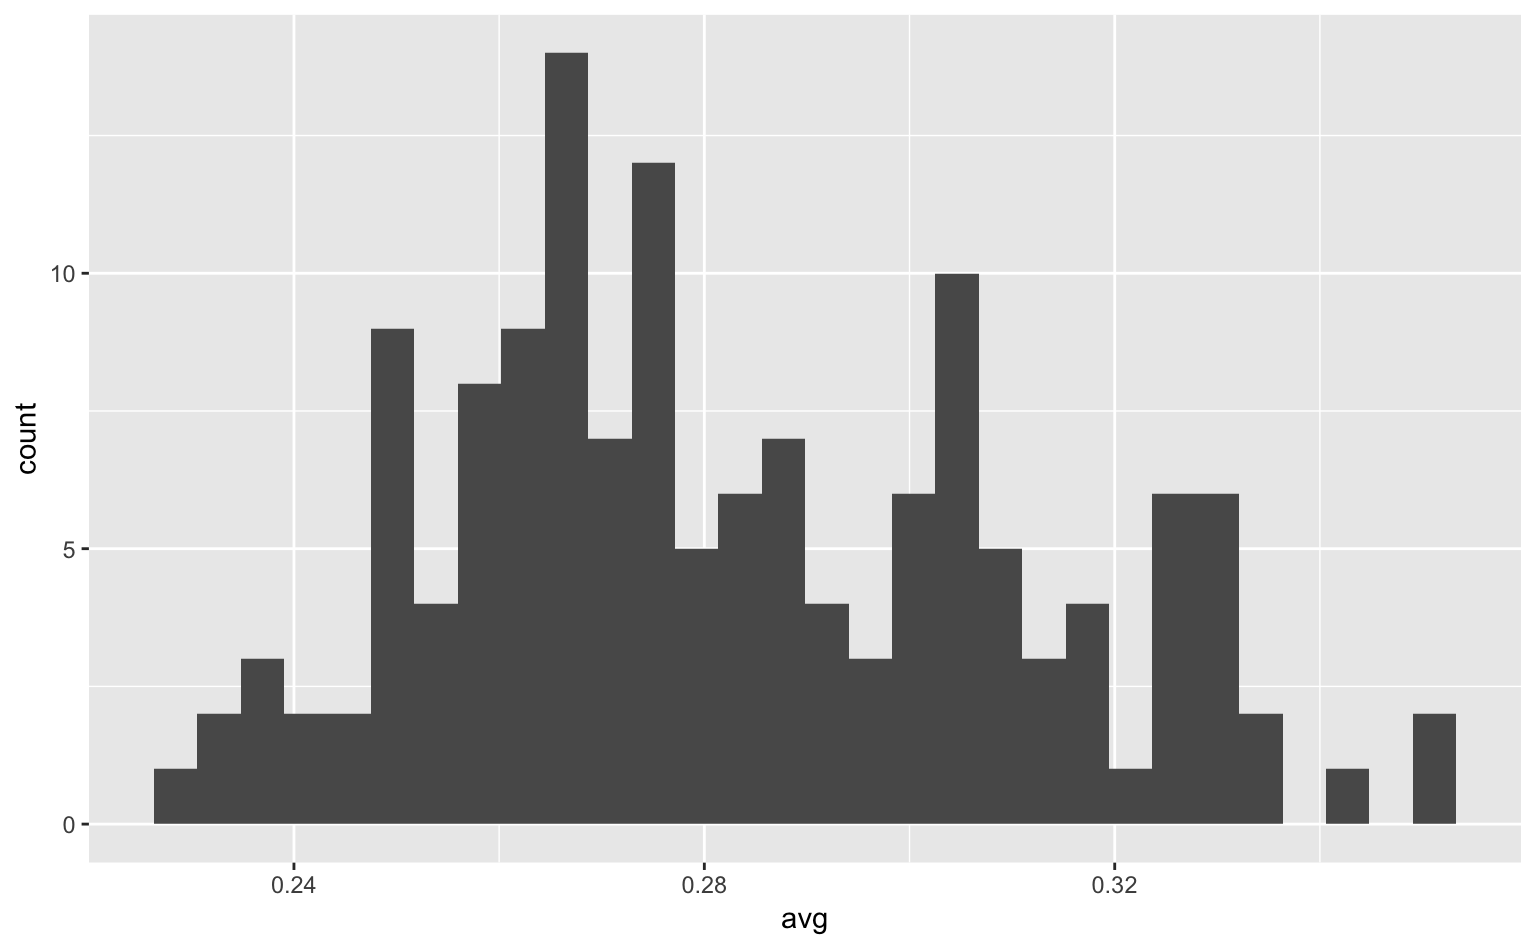
\includegraphics{lecture_note_files/figure-latex/unnamed-chunk-31-1} 

}

\caption{2001年MLBにおける144名の打率の分布。}\label{fig:unnamed-chunk-31}
\end{figure}

グラフを見ると、大体0.28前後が\textbf{中央値}(median)あるいは\textbf{最頻値}(mode)になっていることがわかる。

\begin{center}\rule{0.5\linewidth}{\linethickness}\end{center}

なお、\textbf{ビン}(bin:ヒストグラムの1本1本の棒)の幅を調整することで、分布の印象が大幅に変わるということに注意してほしい。実際、上のグラフを描いた際に、

\texttt{\#\#\ \textasciigrave{}stat\_bin()\textasciigrave{}\ using\ \textasciigrave{}bins\ =\ 30\textasciigrave{}.\ Pick\ better\ value\ with\ \textasciigrave{}binwidth\textasciigrave{}.}

というメッセージが出たかと思う。これはまさにそのことを注意喚起するメッセージである。

データ分析の際は、ビンの幅をいくつか試した上で、最も妥当そうな値を使うようにすると良い。参考に、ビンの幅をそれぞれ0.001、0.01、0.1にした場合の図を下に載せておく。



\begin{Shaded}
\begin{Highlighting}[]
\KeywordTok{ggplot}\NormalTok{(tophitters2001, }\KeywordTok{aes}\NormalTok{(avg)) }\OperatorTok{+}
\StringTok{  }\KeywordTok{geom_histogram}\NormalTok{(}\DataTypeTok{binwidth =} \FloatTok{0.001}\NormalTok{) }\CommentTok{# binwidth = ...でビンの幅を設定}
\end{Highlighting}
\end{Shaded}

\begin{figure}

{\centering 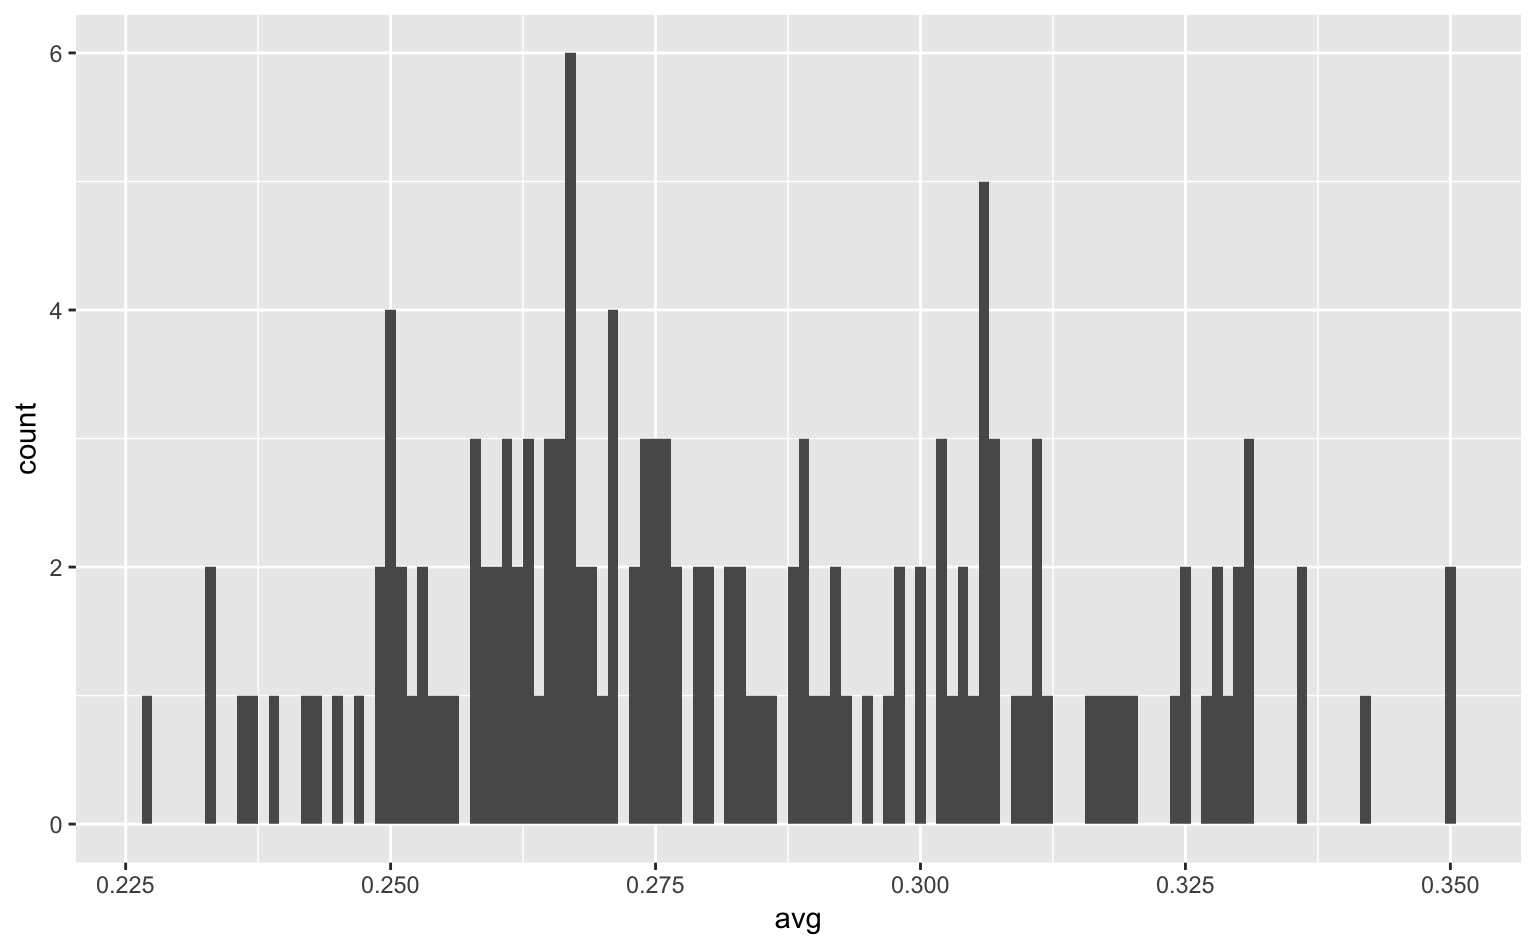
\includegraphics{lecture_note_files/figure-latex/unnamed-chunk-32-1} 

}

\caption{ビンが細すぎるヒストグラム。}\label{fig:unnamed-chunk-32}
\end{figure}



\begin{Shaded}
\begin{Highlighting}[]
\KeywordTok{ggplot}\NormalTok{(tophitters2001, }\KeywordTok{aes}\NormalTok{(avg)) }\OperatorTok{+}
\StringTok{  }\KeywordTok{geom_histogram}\NormalTok{(}\DataTypeTok{binwidth =} \FloatTok{0.01}\NormalTok{) }\CommentTok{# binwidth = ...でビンの幅を設定}
\end{Highlighting}
\end{Shaded}

\begin{figure}

{\centering 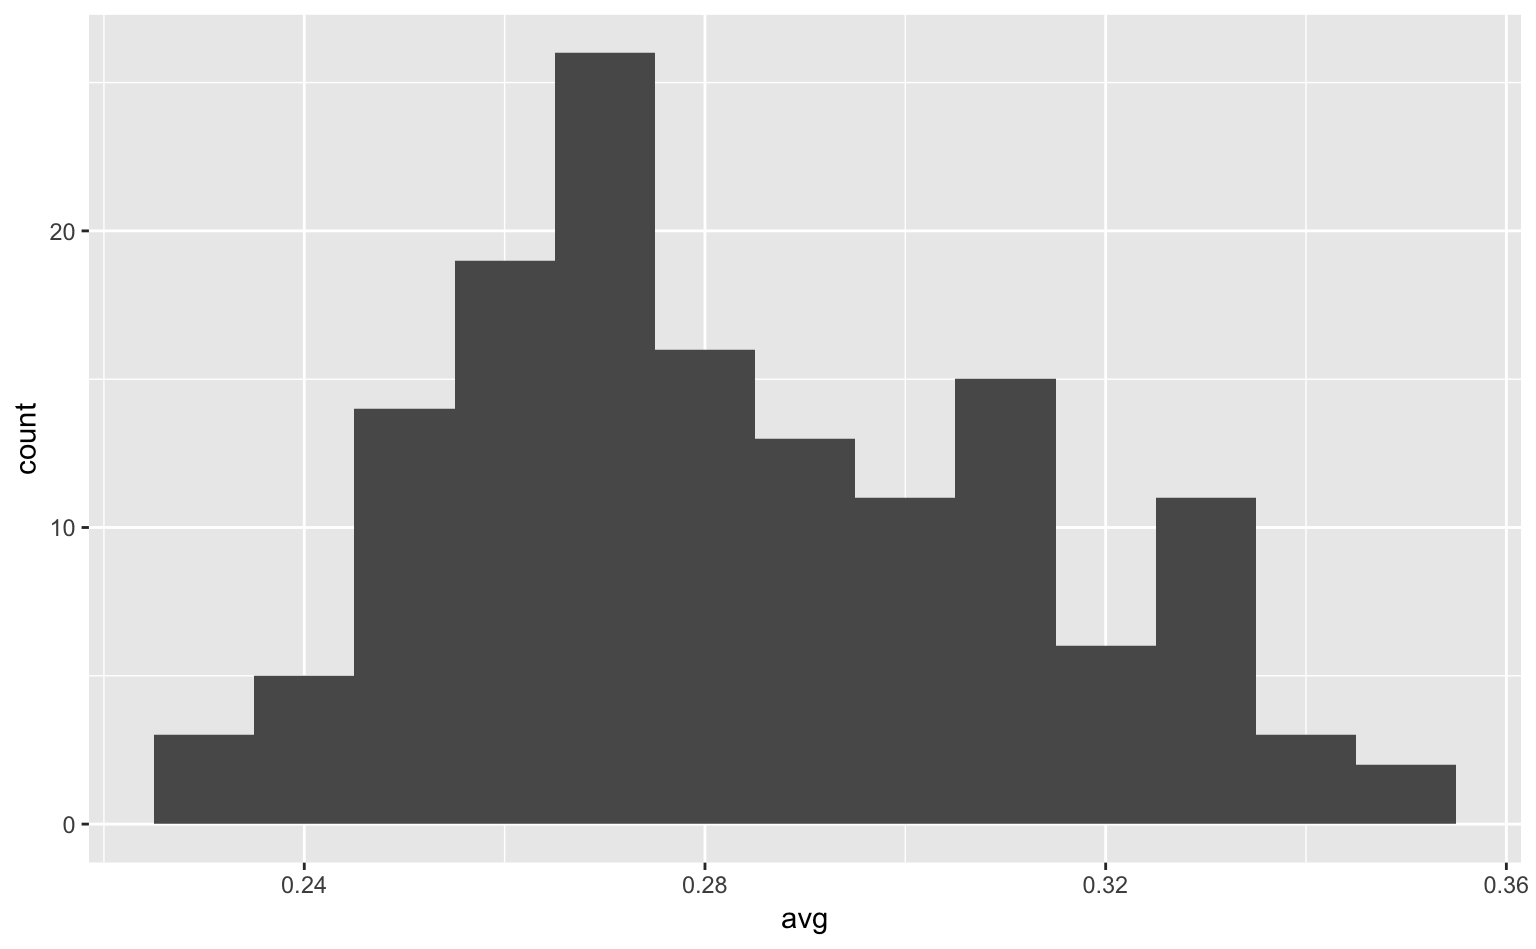
\includegraphics{lecture_note_files/figure-latex/unnamed-chunk-33-1} 

}

\caption{ビンが妥当なサイズのヒストグラム。}\label{fig:unnamed-chunk-33}
\end{figure}



\begin{Shaded}
\begin{Highlighting}[]
\KeywordTok{ggplot}\NormalTok{(tophitters2001, }\KeywordTok{aes}\NormalTok{(avg)) }\OperatorTok{+}
\StringTok{  }\KeywordTok{geom_histogram}\NormalTok{(}\DataTypeTok{binwidth =} \FloatTok{0.1}\NormalTok{) }\CommentTok{# binwidth = ...でビンの幅を設定}
\end{Highlighting}
\end{Shaded}

\begin{figure}

{\centering 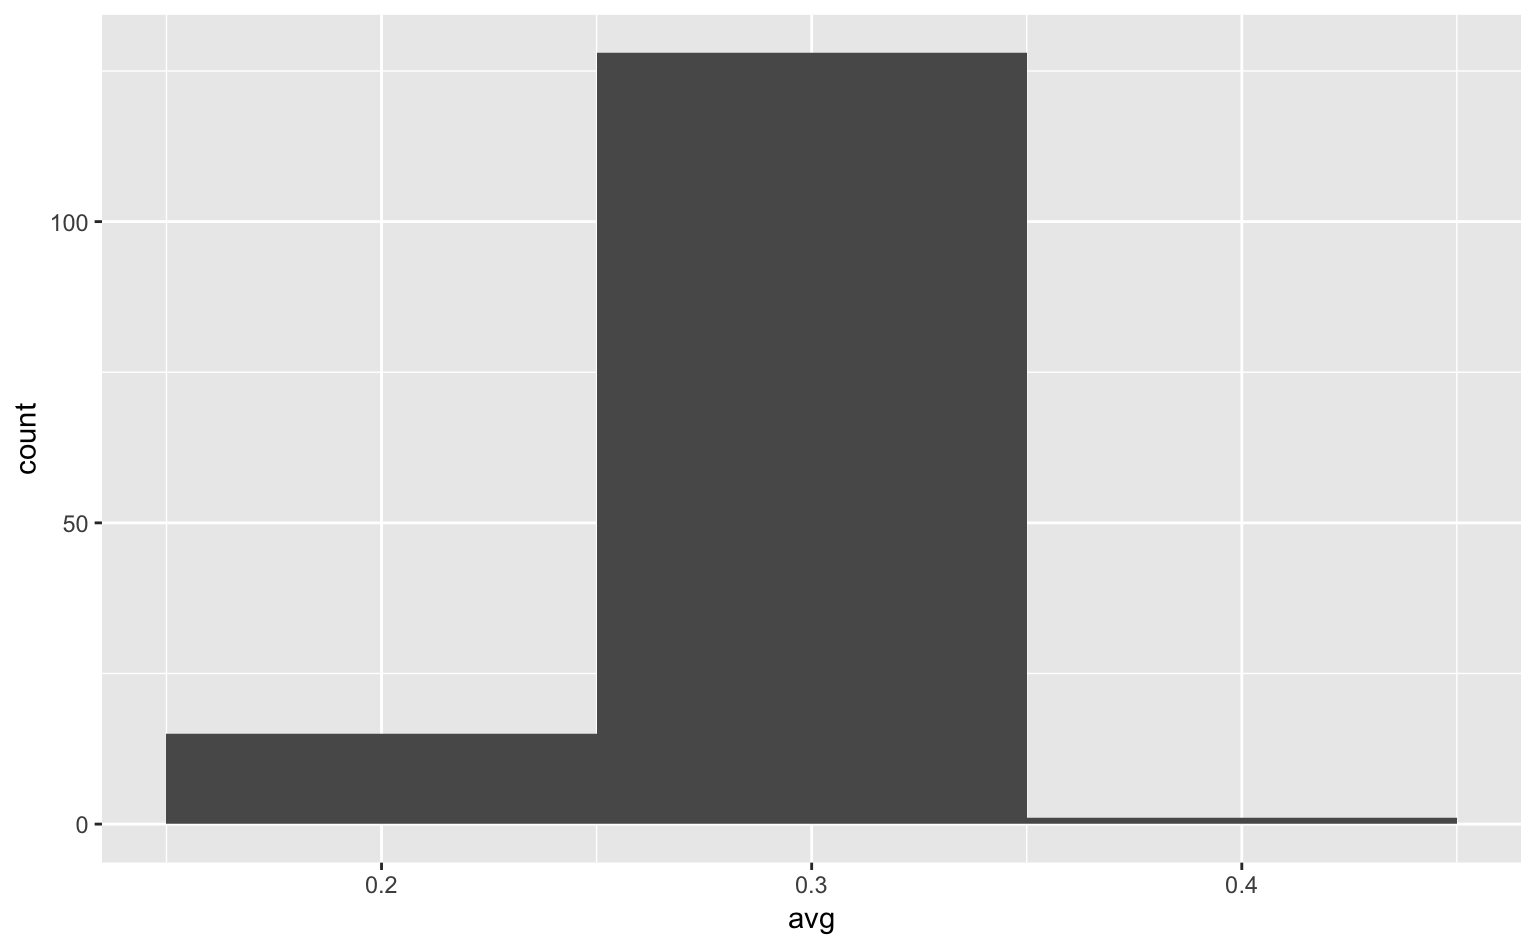
\includegraphics{lecture_note_files/figure-latex/unnamed-chunk-34-1} 

}

\caption{ビンが太すぎるヒストグラム。}\label{fig:unnamed-chunk-34}
\end{figure}

\subsection{グルーピングされたヒストグラム}

たとえば、実験や調査をおこなった際、変数の分布をある集団ごとに見比べたい(グルーピングしたい)ということがあるかと思う。たとえば、「○○の尺度得点の分布は男女間で異なるのでは?」とか、「実験群と統制群とで○○の分布に違いがあるのでは?」などである。

引き続き\texttt{tophitters2001}を使って、その具体例を見てみよう。ここでは、リーグごとの打率の分布を見比べることにする。

\begin{itemize}
\tightlist
\item
  \texttt{lg}:打手の所属リーグ(AL or
  NL;それぞれア・リーグとナ・リーグ)
\end{itemize}

このようなときは、\texttt{fill}にグルーピングしたい変数(\texttt{lg})を指定すれば良い。



\begin{Shaded}
\begin{Highlighting}[]
\KeywordTok{ggplot}\NormalTok{(tophitters2001, }\KeywordTok{aes}\NormalTok{(avg, }\DataTypeTok{fill =}\NormalTok{ lg)) }\OperatorTok{+}\StringTok{ }\CommentTok{# x軸にavg;fillに変数を指定することでグルーピングできる}
\StringTok{  }\KeywordTok{geom_histogram}\NormalTok{(}\DataTypeTok{position =} \StringTok{"identity"}\NormalTok{) }\CommentTok{# position = "identity"としないといけない}
\end{Highlighting}
\end{Shaded}

\begin{figure}

{\centering 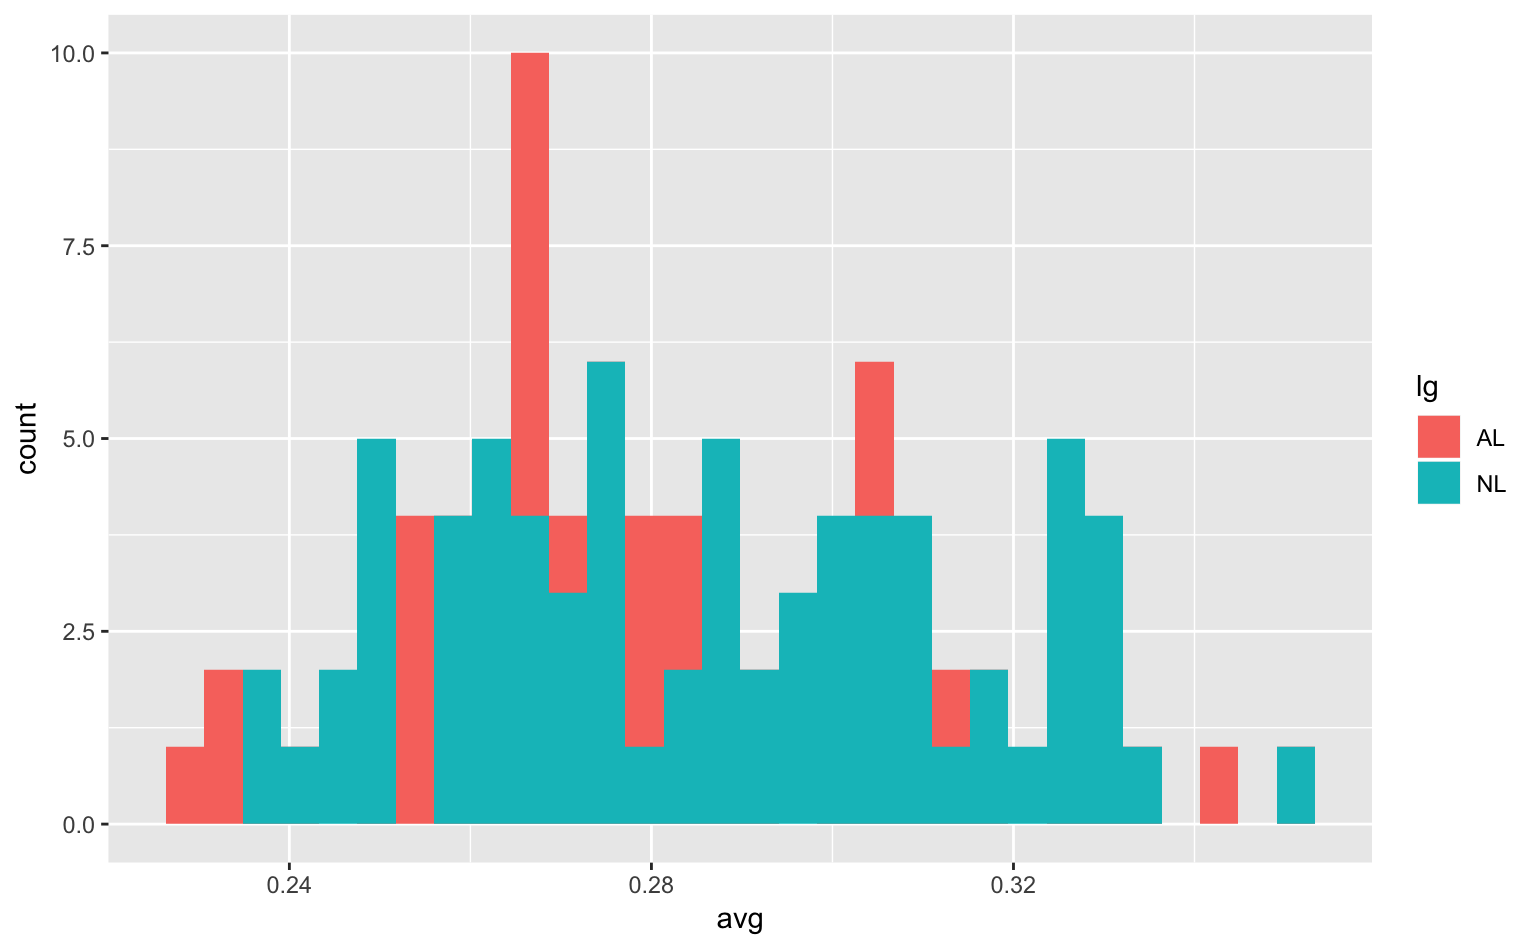
\includegraphics{lecture_note_files/figure-latex/histogram-5-1} 

}

\caption{リーグごとの打率のヒストグラム。}\label{fig:histogram-5}
\end{figure}

なお、ここでは\texttt{position\ =\ "identity"}と設定しなくてはならない。なぜなら、\texttt{geom\_histogram()}は\texttt{position\ =\ "stack"}がデフォルト設定であり、そのままだと積み上げ棒グラフのようになってしまうからである。気になる人は、\texttt{position\ =\ "identity"}の部分を消した上で、もう一度グラフを描いてみよう。

また、基本的には上のヒストグラムでも問題ないが、ア・リーグのデータがナ・リーグの後ろに隠れてしまっているのが若干気になる。このようなときは、\texttt{alpha}に0〜1の値を指定すると、ヒストグラムが半透明になり、上の問題を解決できる。



\begin{Shaded}
\begin{Highlighting}[]
\KeywordTok{ggplot}\NormalTok{(tophitters2001, }\KeywordTok{aes}\NormalTok{(avg, }\DataTypeTok{fill =}\NormalTok{ lg)) }\OperatorTok{+}
\StringTok{  }\KeywordTok{geom_histogram}\NormalTok{(}\DataTypeTok{position =} \StringTok{"identity"}\NormalTok{, }\DataTypeTok{alpha =} \FloatTok{0.7}\NormalTok{) }\CommentTok{# 0だと完全に透明、1だと完全に不透明}
\end{Highlighting}
\end{Shaded}

\begin{figure}

{\centering 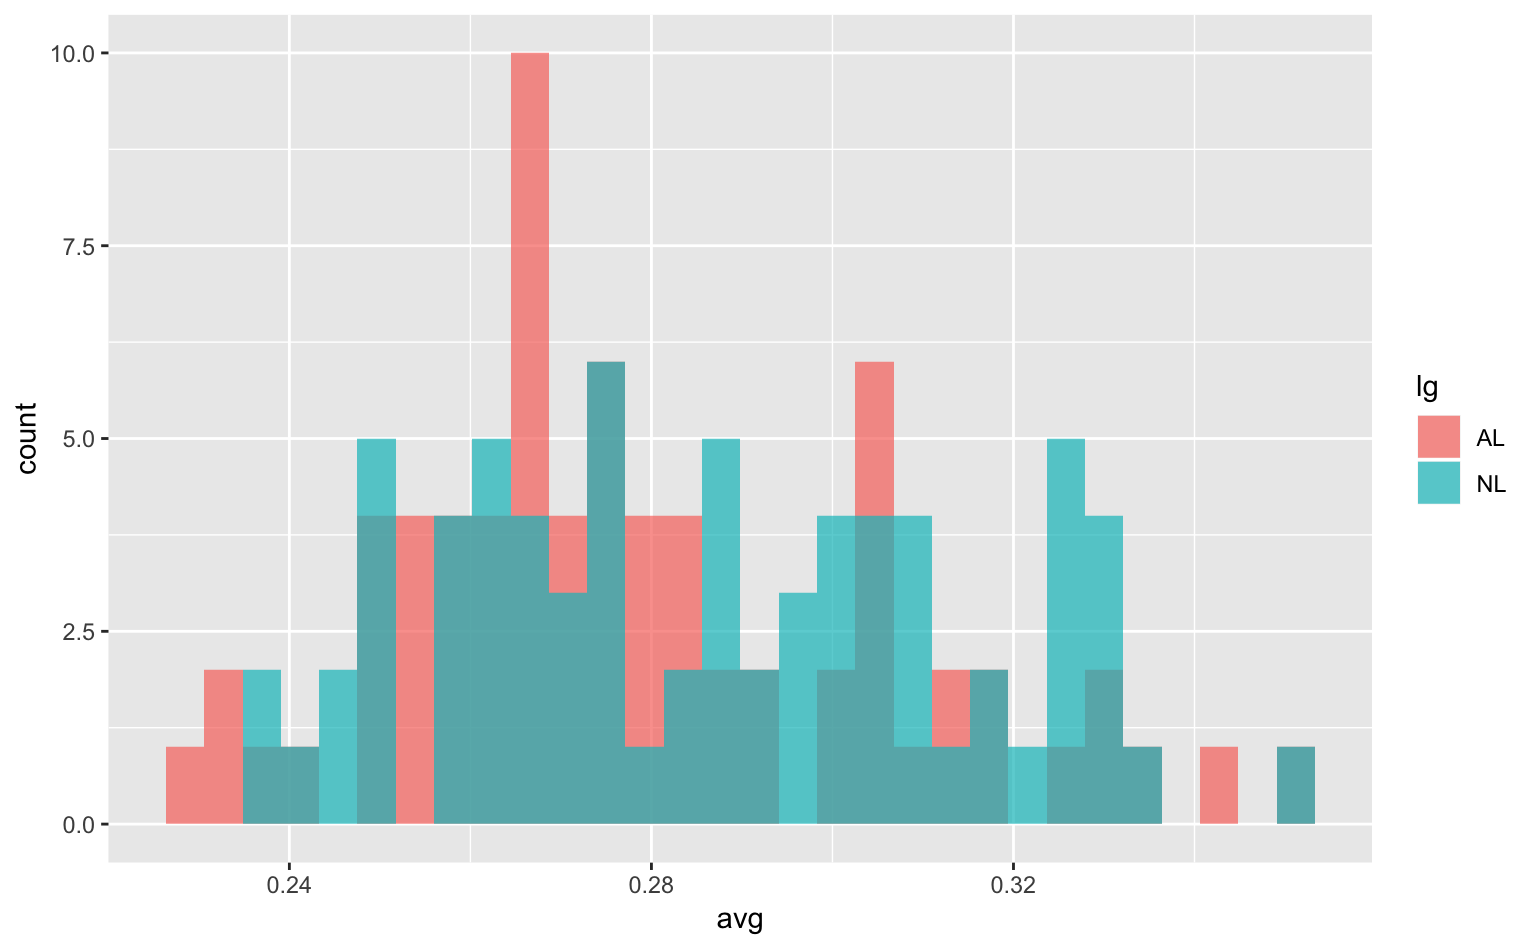
\includegraphics{lecture_note_files/figure-latex/unnamed-chunk-35-1} 

}

\caption{Figure \ref{fig:histogram-5}を半透明にしたもの。}\label{fig:unnamed-chunk-35}
\end{figure}

無事ア・リーグのデータが見えるようになった。

\section{密度プロット}

ヒストグラムと似たようなグラフに、\textbf{密度プロット}(density
plot)がある。密度プロットとは、ヒストグラムのようにローデータ(raw
data)をそのままプロットするのではなく、カーネル密度推定(kernel-density
estimation)というテクニックで密度分布を推定した上で可視化する手法である。グラフが手書きの時代だった頃からヒストグラムがあるのに対し、密度プロットは計算機の発達によって開発された比較的新しいグラフである。

描き方は簡単で、上で\texttt{geom\_histogram()}としていたところを\texttt{geom\_density()}に差し替えるだけで良い。



\begin{Shaded}
\begin{Highlighting}[]
\KeywordTok{ggplot}\NormalTok{(tophitters2001, }\KeywordTok{aes}\NormalTok{(avg, }\DataTypeTok{fill =}\NormalTok{ lg)) }\OperatorTok{+}\StringTok{ }\CommentTok{# x軸にavg;fillに変数を指定することでグルーピングできる}
\StringTok{  }\KeywordTok{geom_density}\NormalTok{(}\DataTypeTok{alpha =} \FloatTok{0.7}\NormalTok{) }\CommentTok{# デフォルトがposition = "identity"なので、geom_histogram(position = "identity")のように明示的に指定する必要がない}
\end{Highlighting}
\end{Shaded}

\begin{figure}

{\centering 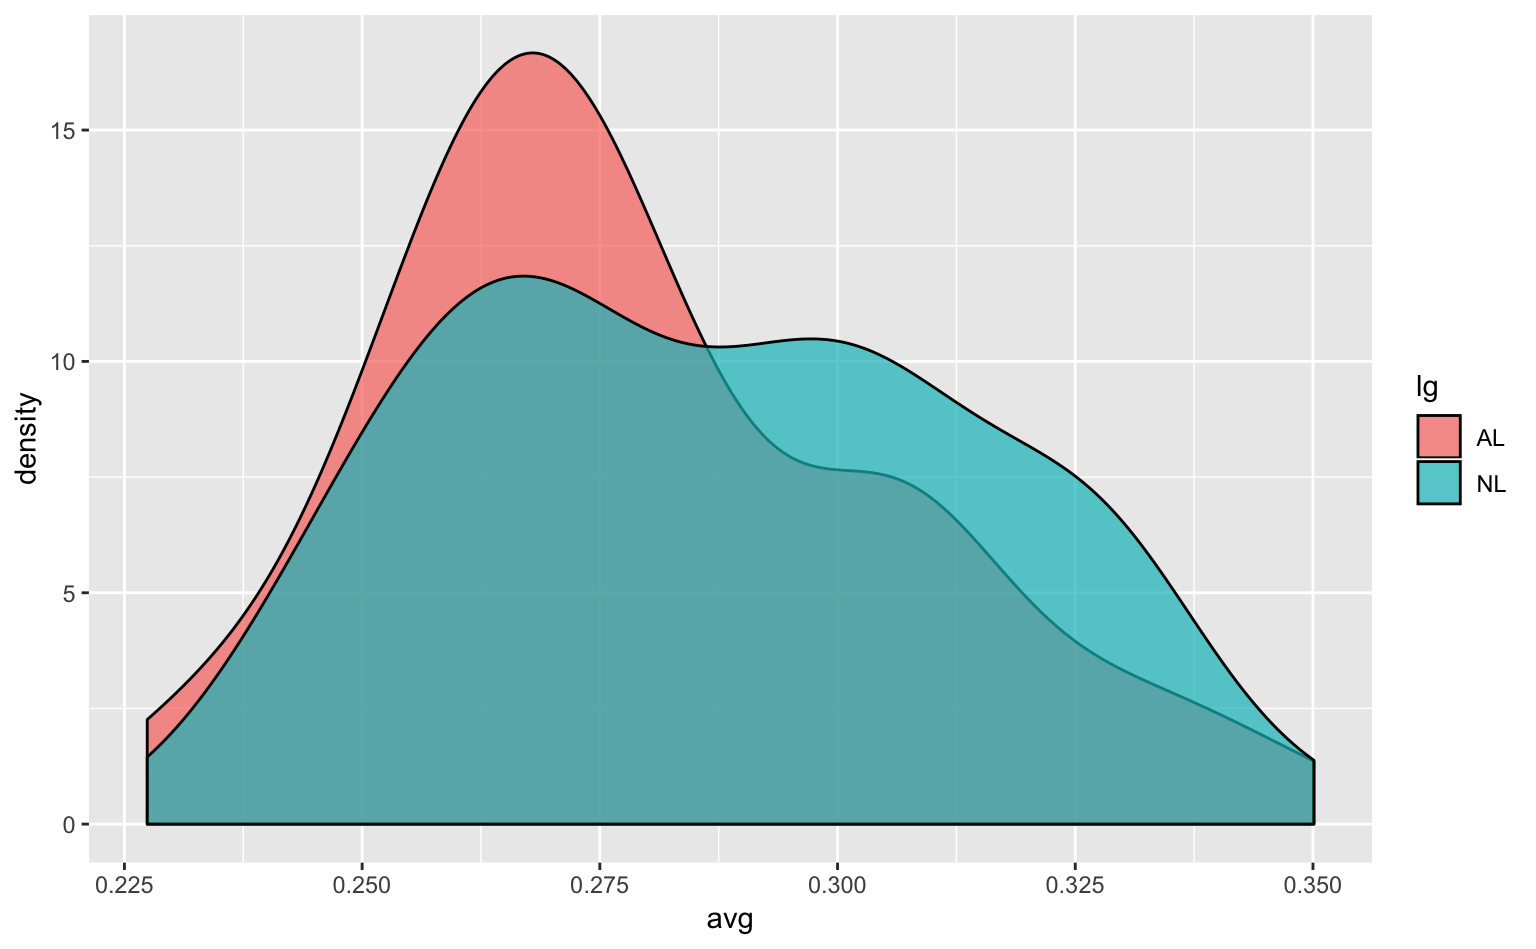
\includegraphics{lecture_note_files/figure-latex/unnamed-chunk-36-1} 

}

\caption{リーグごとの打率の密度プロット。}\label{fig:unnamed-chunk-36}
\end{figure}

y軸は推定された密度を表している(5人とか10人といった人数を表しているわけではない)。この密度は、塗りつぶされた面積の総和が1になるように算出されているだけなので、値そのものにはあまり意味がないことに注意してほしい。

また、密度プロットもヒストグラムと同様に、描き方次第ではデータの性質を捉えきれないという欠点がある。\texttt{geom\_histogram()}では\texttt{binwidth}を調整する必要があったが、\texttt{geom\_density()}では\texttt{adjust}という引数(カーネル密度推定に用いられるパラメタ)を調整する必要がある。先程と同様に、\texttt{adjust}の値をそれぞれ0.25,
1, 4にしたグラフを下に載せておく。

(ref:density-plot-2)
平滑化が弱すぎる密度プロット。データの全体的な特徴が見えにくくなってしまっている。

\begin{Shaded}
\begin{Highlighting}[]
\KeywordTok{ggplot}\NormalTok{(tophitters2001, }\KeywordTok{aes}\NormalTok{(avg, }\DataTypeTok{fill =}\NormalTok{ lg)) }\OperatorTok{+}
\StringTok{  }\KeywordTok{geom_density}\NormalTok{(}\DataTypeTok{alpha =} \FloatTok{0.7}\NormalTok{, }\DataTypeTok{adjust =} \FloatTok{0.25}\NormalTok{) }\CommentTok{# adjust = ...で平滑化の強度を調整}
\end{Highlighting}
\end{Shaded}

\begin{figure}

{\centering 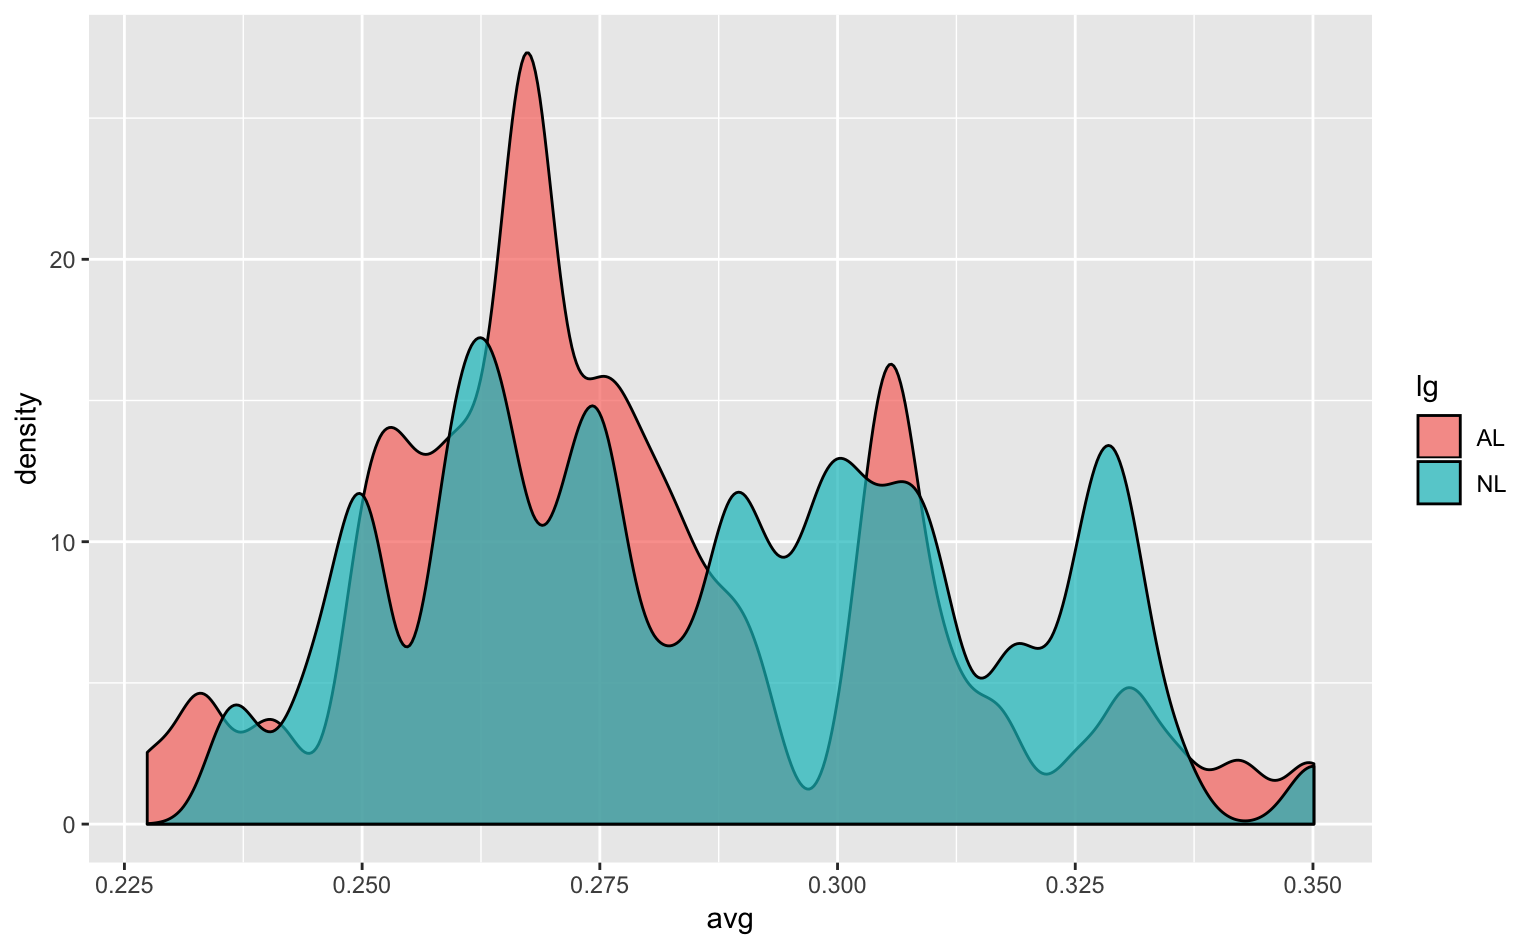
\includegraphics{lecture_note_files/figure-latex/unnamed-chunk-37-1} 

}

\caption{(ref:density-plot-2)}\label{fig:unnamed-chunk-37}
\end{figure}



\begin{Shaded}
\begin{Highlighting}[]
\KeywordTok{ggplot}\NormalTok{(tophitters2001, }\KeywordTok{aes}\NormalTok{(avg, }\DataTypeTok{fill =}\NormalTok{ lg)) }\OperatorTok{+}
\StringTok{  }\KeywordTok{geom_density}\NormalTok{(}\DataTypeTok{alpha =} \FloatTok{0.7}\NormalTok{, }\DataTypeTok{adjust =} \DecValTok{1}\NormalTok{) }\CommentTok{# adjust = ...で平滑化の強度を調整}
\end{Highlighting}
\end{Shaded}

\begin{figure}

{\centering 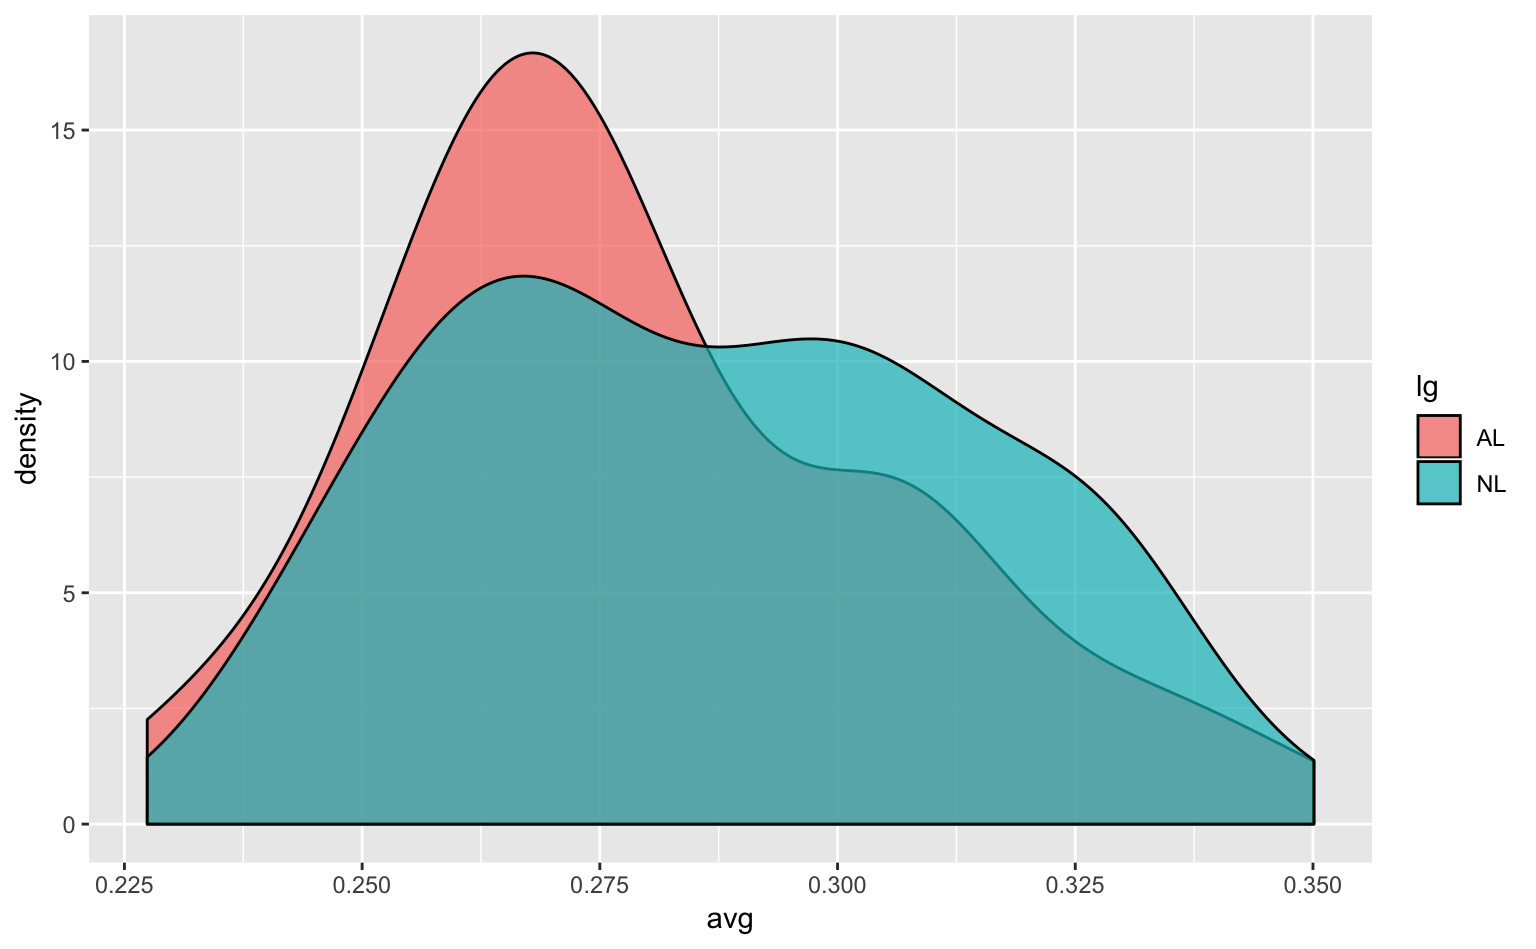
\includegraphics{lecture_note_files/figure-latex/unnamed-chunk-38-1} 

}

\caption{妥当な平滑化の密度プロット(デフォルトの設定)。}\label{fig:unnamed-chunk-38}
\end{figure}

(ref:density-plot-4)
平滑化が強すぎる密度プロット。データを平滑化しすぎており、分布の違いが見えなくなってしまっている。

\begin{Shaded}
\begin{Highlighting}[]
\KeywordTok{ggplot}\NormalTok{(tophitters2001, }\KeywordTok{aes}\NormalTok{(avg, }\DataTypeTok{fill =}\NormalTok{ lg)) }\OperatorTok{+}
\StringTok{  }\KeywordTok{geom_density}\NormalTok{(}\DataTypeTok{alpha =} \FloatTok{0.7}\NormalTok{, }\DataTypeTok{adjust =} \DecValTok{4}\NormalTok{) }\CommentTok{# adjust = ...で平滑化の強度を調整}
\end{Highlighting}
\end{Shaded}

\begin{figure}

{\centering 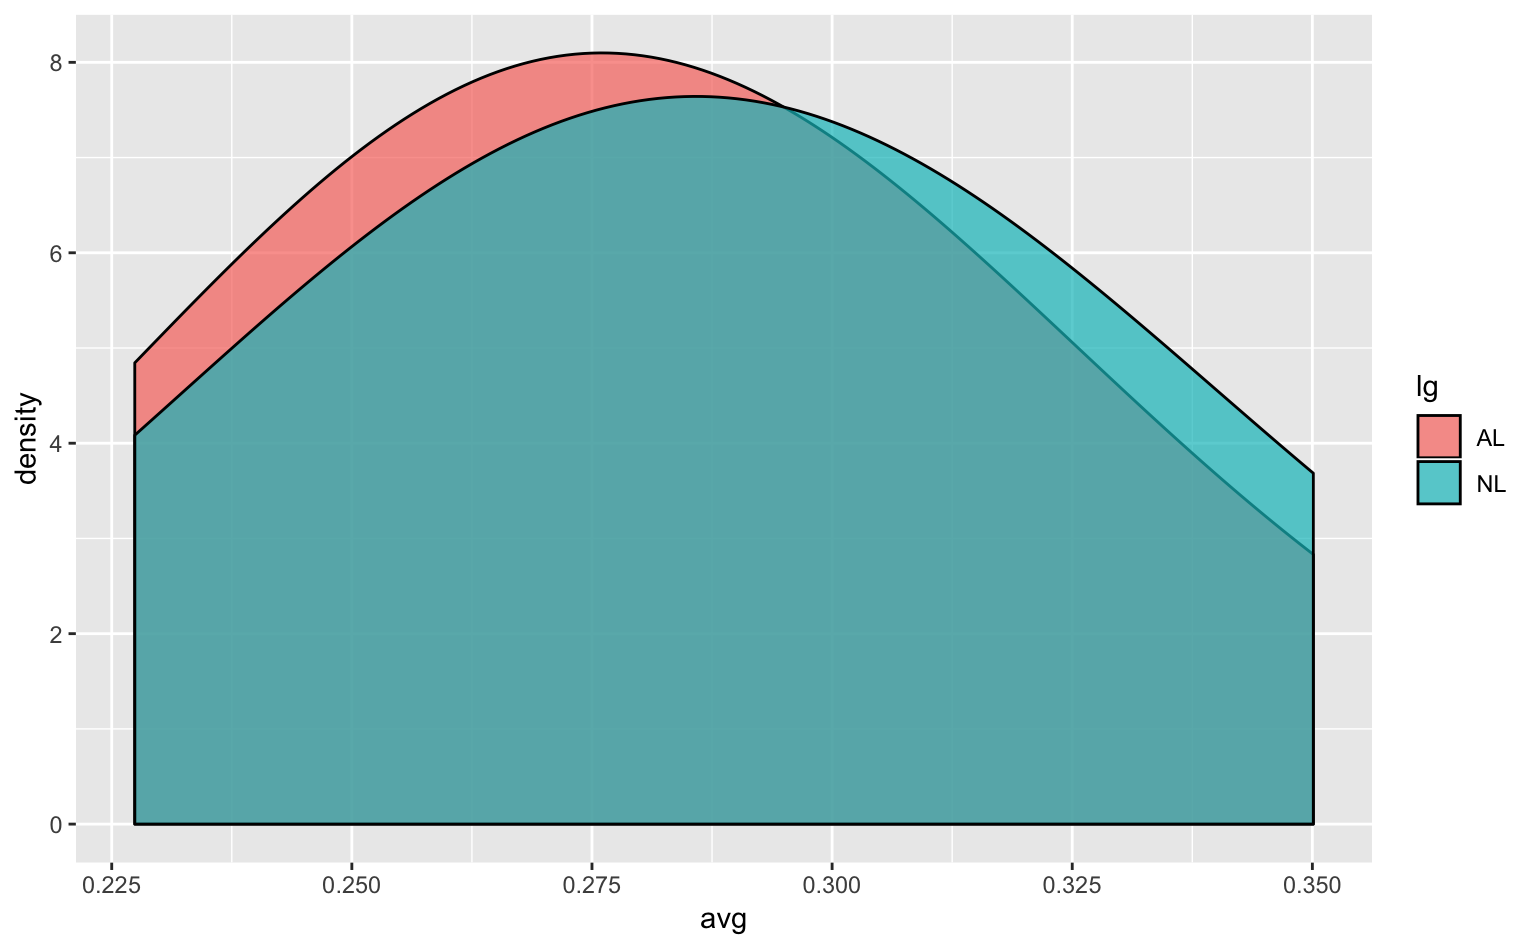
\includegraphics{lecture_note_files/figure-latex/unnamed-chunk-39-1} 

}

\caption{(ref:density-plot-4)}\label{fig:unnamed-chunk-39}
\end{figure}

\begin{center}\rule{0.5\linewidth}{\linethickness}\end{center}

ところで、Chapter
\ref{tutorial}でも少し述べたように、\textbf{ggplot2では複数のプロットを重ね合わせることができる。}たとえば、ヒストグラムと密度プロットは以下のように重ね合わせることができる。



\begin{Shaded}
\begin{Highlighting}[]
\KeywordTok{ggplot}\NormalTok{(tophitters2001, }\KeywordTok{aes}\NormalTok{(avg, }\DataTypeTok{y =}\NormalTok{ ..density..)) }\OperatorTok{+}\StringTok{ }\CommentTok{# y = ..density..とする必要あり}
\StringTok{  }\KeywordTok{geom_histogram}\NormalTok{(}\DataTypeTok{binwidth =} \FloatTok{0.01}\NormalTok{) }\OperatorTok{+}\StringTok{ }\CommentTok{# まずヒストグラムを描く}
\StringTok{  }\KeywordTok{geom_density}\NormalTok{(}\DataTypeTok{alpha =} \FloatTok{0.7}\NormalTok{) }\CommentTok{# その上に密度プロットを描く}
\end{Highlighting}
\end{Shaded}

\begin{figure}

{\centering 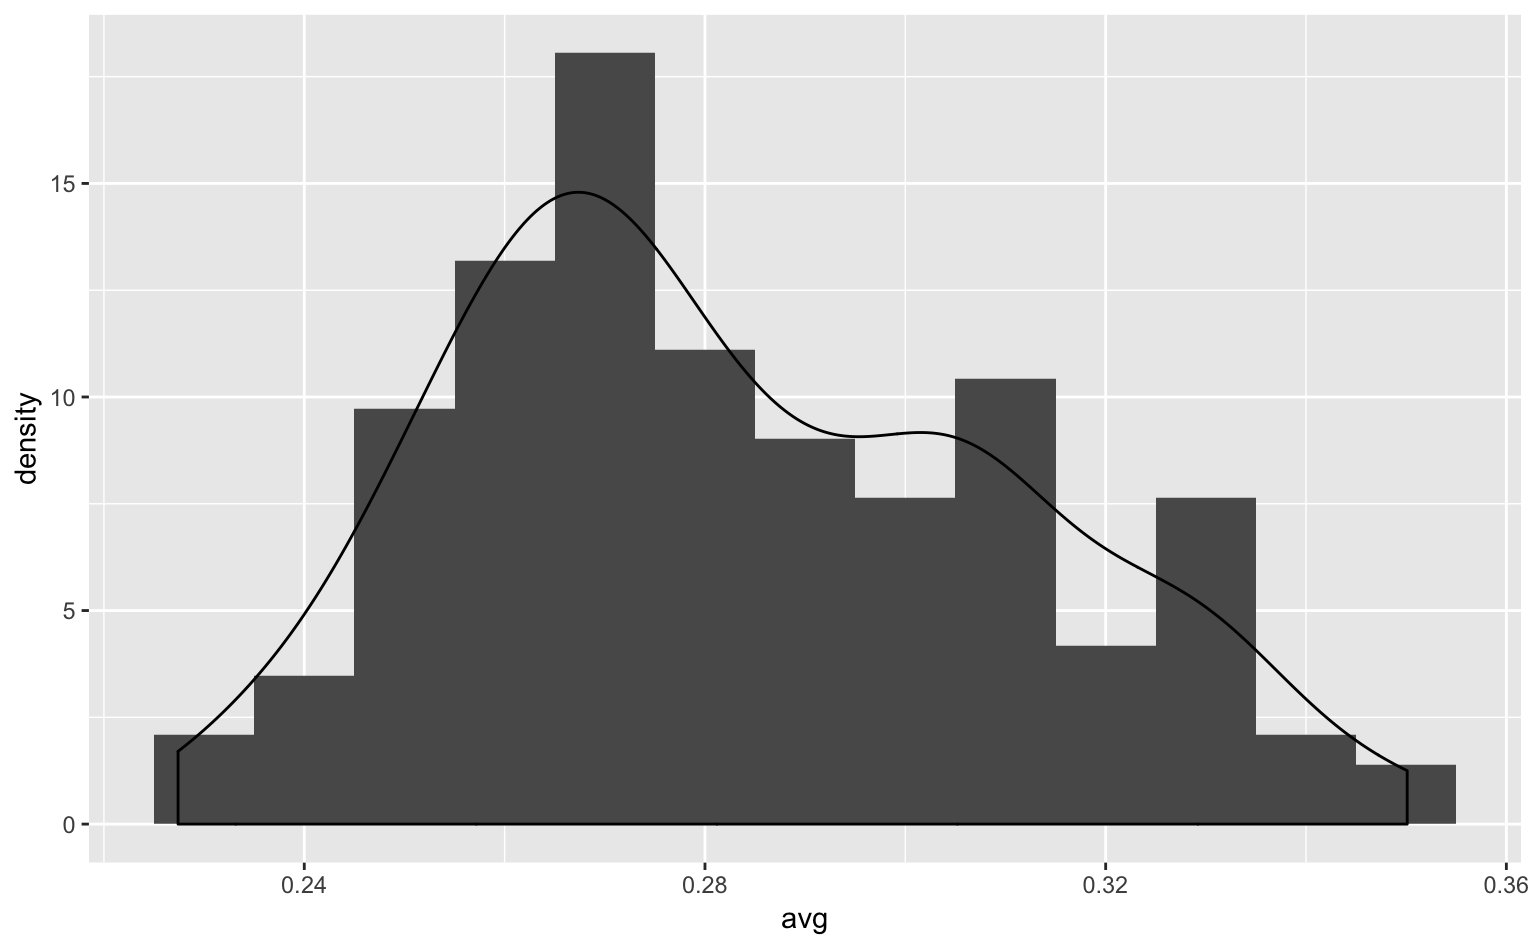
\includegraphics{lecture_note_files/figure-latex/unnamed-chunk-40-1} 

}

\caption{ヒストグラムと密度プロットを重ねたグラフ。}\label{fig:unnamed-chunk-40}
\end{figure}

なお、ここでは\texttt{y\ =\ ..density..}をコードに追加する必要がある。なぜなら、\texttt{geom\_density()}が密度をy軸に取るのに対し、\texttt{geom\_histogram()}はデフォルトでデータの個数をy軸に取ってしまうからである。2つのプロットのy軸の単位を揃えるために、ここでは「データの密度(\texttt{..density..})をy軸に取ってください」と明示的に指定しなければならない。

\section{箱ひげ図}

ヒストグラムや密度プロットとは異なり、データの要約統計量を示しつつ、同時に分布を表せるようなグラフも存在する。その代表例は\textbf{箱ひげ図}(box
plot; box-and-whisker plot)だろう。

ここではRにデフォルトで搭載されている\texttt{PlantGrowth}(植物の重さに関する実験のデータセット)を使うことにする。

\begin{Shaded}
\begin{Highlighting}[]
\KeywordTok{head}\NormalTok{(PlantGrowth) }\CommentTok{# 先頭6行を確認}
\end{Highlighting}
\end{Shaded}

\begin{verbatim}
##   weight group
## 1   4.17  ctrl
## 2   5.58  ctrl
## 3   5.18  ctrl
## 4   6.11  ctrl
## 5   4.50  ctrl
## 6   4.61  ctrl
\end{verbatim}

このデータには2つの変数があり、それぞれ

\begin{itemize}
\item
  \texttt{group}:実験の条件(ctrl, trt1, or trt2)
\item
  \texttt{weight}:植物の重さ
\end{itemize}

を表している。

さて、3つの条件ごとに植物の重さの分布を可視化したい。もちろんヒストグラムや密度プロットでもよいが、ここでは箱ひげ図を使ってみよう。以下のコードで箱ひげ図を描くことができる。なお、箱ひげ図に色をつけるには\texttt{fill}に変数を指定すれば良い。



\begin{Shaded}
\begin{Highlighting}[]
\KeywordTok{ggplot}\NormalTok{(PlantGrowth, }\KeywordTok{aes}\NormalTok{(group, weight, }\DataTypeTok{fill =}\NormalTok{ group)) }\OperatorTok{+}\StringTok{ }\CommentTok{# x軸にgroup、y軸にweight;fillで色の塗りつぶし}
\StringTok{  }\KeywordTok{geom_boxplot}\NormalTok{() }\CommentTok{# 箱ひげ図を描くためのコード}
\end{Highlighting}
\end{Shaded}

\begin{figure}

{\centering 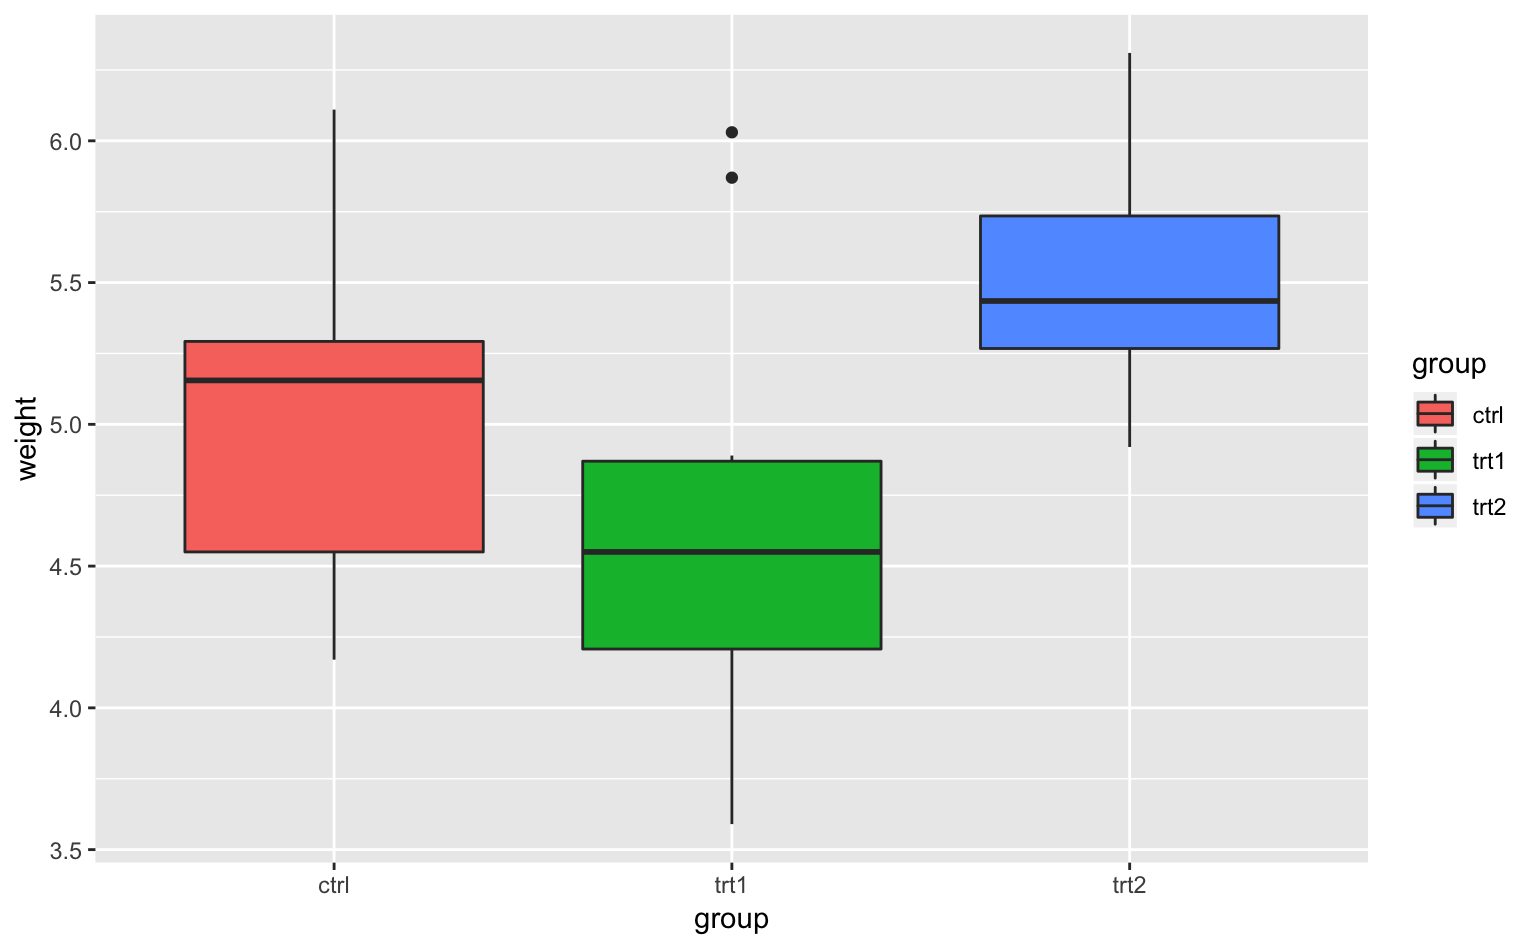
\includegraphics{lecture_note_files/figure-latex/boxplot-1-1} 

}

\caption{箱ひげ図。x軸は条件、y軸は植物の重さを表している。}\label{fig:boxplot-1}
\end{figure}

何やら謎の図形が現れたが、まさにこれが箱ひげ図である。図形のそれぞれのパーツは以下のものを表している\footnote{色々なスタイル・流派があるらしいが、ここでは最もよく使われるTukeyの箱ひげ図を説明している。}。

\begin{itemize}
\item
  四角(箱):四分位範囲(interquartile range,
  IQR)。25パーセンタイルから75パーセンタイルのこと
\item
  縦線(ひげ):四角の上端/下端からIQR × 1.5の範囲
\item
  太線:中央値。50パーセンタイル(percentile)とも言う
\item
  点:外れ値(outlier;IQR × 1.5より外側の値)
\end{itemize}

英語版Wikipedia ``Interquartile
range''(\url{https://en.wikipedia.org/wiki/Interquartile_range})
の図が説明としてわかりやすいだろう。

\begin{center}\rule{0.5\linewidth}{\linethickness}\end{center}

ただし、箱ひげ図だけではデータの平均値を描くことができない\footnote{平均値は外れ値に引っ張られるので、分布の代表値としては中央値のほうが妥当な場合が多い。箱ひげ図がデフォルトで平均値を描かないのもおそらくはそのため。}。平均値を追加するには、以下のコードを書けば良い。



\begin{Shaded}
\begin{Highlighting}[]
\KeywordTok{ggplot}\NormalTok{(PlantGrowth, }\KeywordTok{aes}\NormalTok{(group, weight, }\DataTypeTok{fill =}\NormalTok{ group)) }\OperatorTok{+}
\StringTok{  }\KeywordTok{geom_boxplot}\NormalTok{() }\OperatorTok{+}
\StringTok{  }\KeywordTok{stat_summary}\NormalTok{(}\DataTypeTok{geom =} \StringTok{"point"}\NormalTok{, }\DataTypeTok{fun.y =}\NormalTok{ mean, }\DataTypeTok{color =} \StringTok{"white"}\NormalTok{, }\DataTypeTok{shape =} \StringTok{"diamond"}\NormalTok{, }\DataTypeTok{size =} \DecValTok{3}\NormalTok{) }\CommentTok{# 各引数の意味はなんとなく解読してほしい}
\end{Highlighting}
\end{Shaded}

\begin{figure}

{\centering 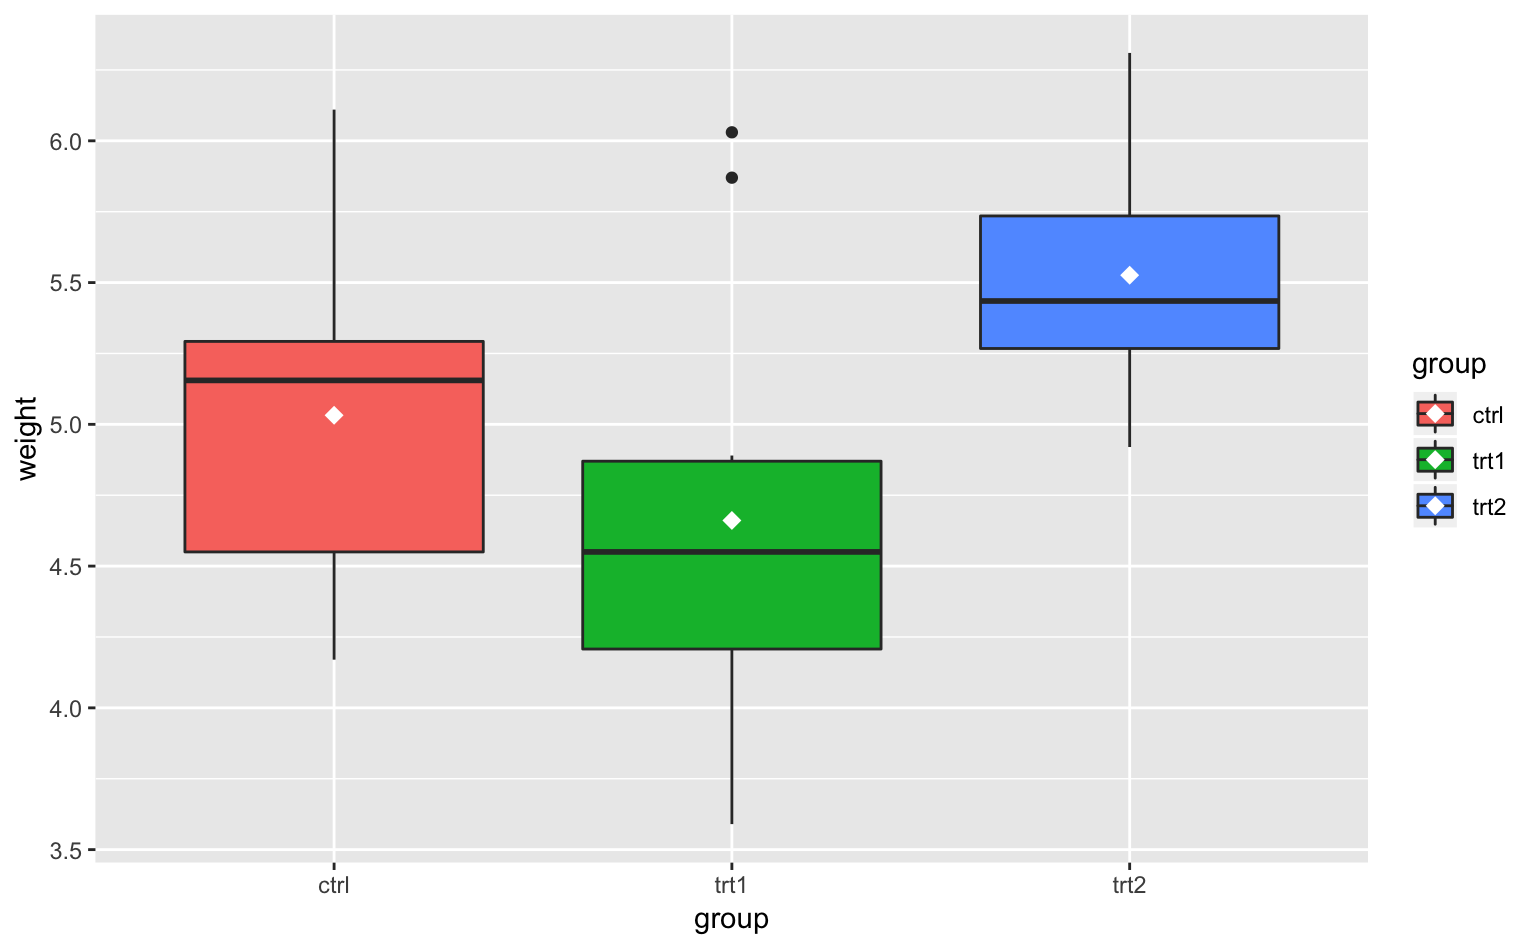
\includegraphics{lecture_note_files/figure-latex/unnamed-chunk-42-1} 

}

\caption{平均値を追加した箱ひげ図。}\label{fig:unnamed-chunk-42}
\end{figure}

\texttt{stat\_summary()}は統計量をプロットするための関数である。このグラフでは「\texttt{y}(\texttt{weight})の平均値をサイズ3の白いひし形で描いてください」と指示している。各引数の意味はなんとなくわかると思うので、説明は割愛する。

\section{バイオリンプロット}

箱ひげ図に似たものとして、\textbf{バイオリンプロット}(violin
plot)がある。バイオリンプロットとは、密度プロットを90°回転させ、アジの干物のように開いたグラフである。

バイオリンプロットは、\texttt{geom\_violin()}で描くことができる。

(ref:violin-plot)
バイオリンプロット。x軸は条件、y軸は植物の重さを表している。

\begin{Shaded}
\begin{Highlighting}[]
\KeywordTok{ggplot}\NormalTok{(PlantGrowth, }\KeywordTok{aes}\NormalTok{(group, weight, }\DataTypeTok{fill =}\NormalTok{ group)) }\OperatorTok{+}\StringTok{ }\CommentTok{# x軸にgroup、y軸にweight、fillで塗りつぶし}
\StringTok{  }\KeywordTok{geom_violin}\NormalTok{() }\CommentTok{# バイオリンプロットを描くためのコード}
\end{Highlighting}
\end{Shaded}

\begin{figure}

{\centering 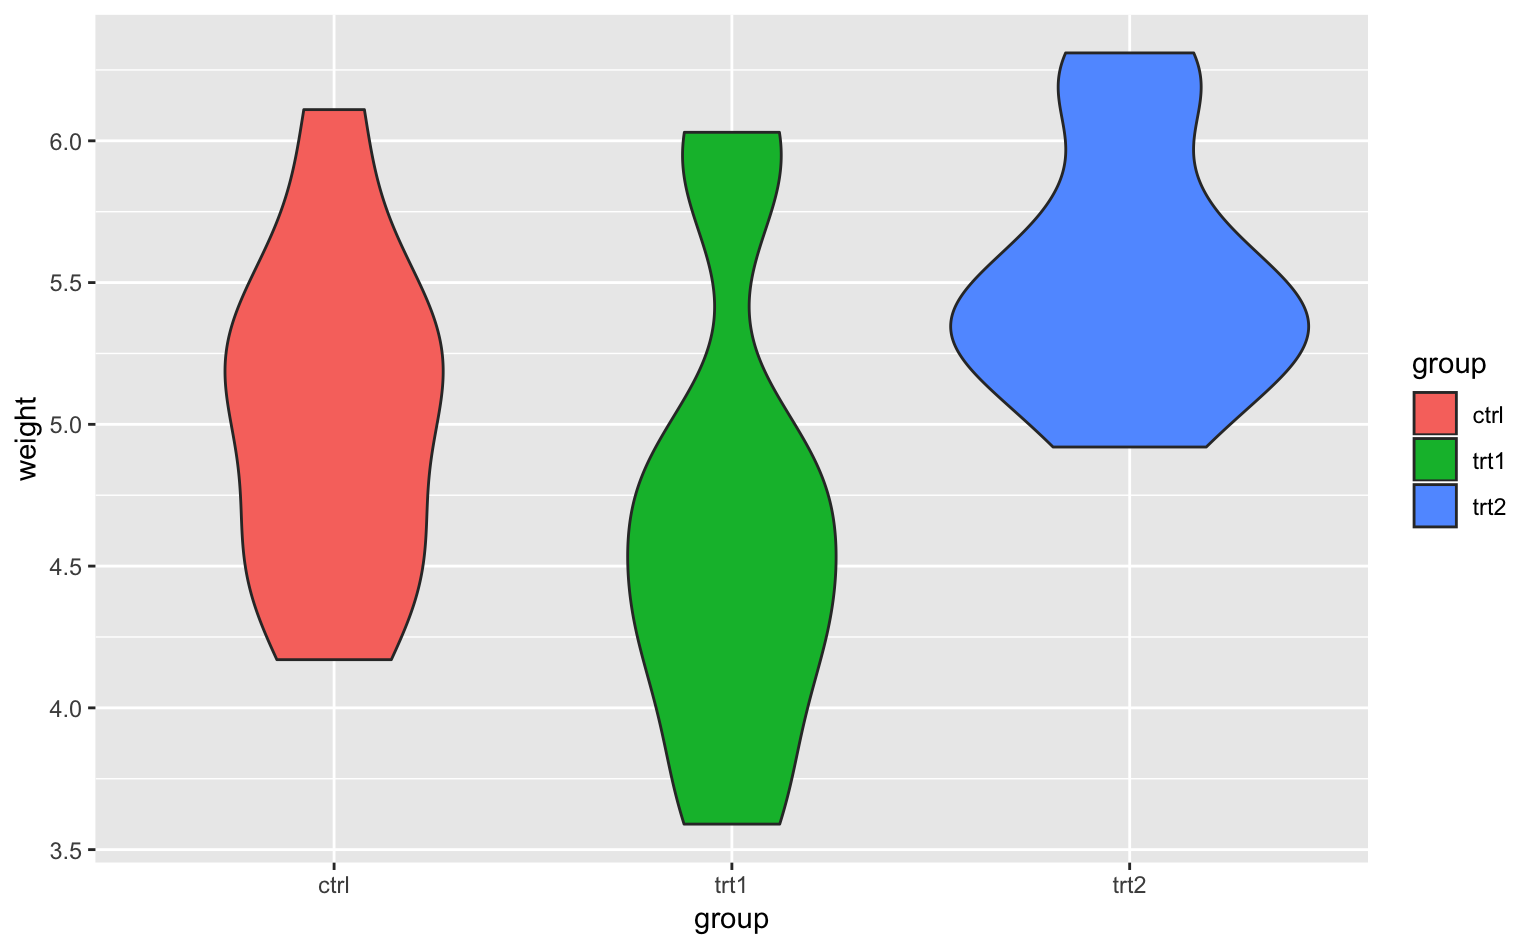
\includegraphics{lecture_note_files/figure-latex/unnamed-chunk-43-1} 

}

\caption{(ref:violin-plot)}\label{fig:unnamed-chunk-43}
\end{figure}

このように、バイオリンプロットを使うと、分布の形状が箱ひげ図よりも直観的にわかるようになる。なお、\texttt{geom\_density()}と同様に、\texttt{geom\_violin()}でも、カーネル密度推定用のパラメタ(\texttt{adjust})をいじることができるので、いくつか試してみてほしい。

\section{ストリッププロット}

箱ひげ図/バイオリンプロットは、\textbf{ストリッププロット}(strip
plot)とも相性が良い。ストリッププロットとは、1つ1つのデータをそのままドットとして表現したグラフである。この説明ではイメージが湧きにくいと思うので、とりあえず下のプロットを見てほしい。

(ref:strip-plot)
ストリッププロットを箱ひげ図とバイオリンプロットの上に重ね合わせた図。ドットはデータそのものを表している。

\begin{Shaded}
\begin{Highlighting}[]
\KeywordTok{ggplot}\NormalTok{(PlantGrowth, }\KeywordTok{aes}\NormalTok{(group, weight, }\DataTypeTok{fill =}\NormalTok{ group)) }\OperatorTok{+}\StringTok{ }\CommentTok{# x軸にgroup、y軸にweight、fillで塗りつぶし}
\StringTok{  }\KeywordTok{geom_violin}\NormalTok{() }\OperatorTok{+}\StringTok{ }\CommentTok{# まずバイオリンプロット}
\StringTok{  }\KeywordTok{geom_boxplot}\NormalTok{(}\DataTypeTok{outlier.shape =} \OtherTok{NA}\NormalTok{, }\DataTypeTok{width =} \FloatTok{0.2}\NormalTok{) }\OperatorTok{+}\StringTok{ }\CommentTok{# その上に箱ひげ図}
\StringTok{  }\KeywordTok{geom_point}\NormalTok{(}\DataTypeTok{position =} \KeywordTok{position_jitter}\NormalTok{(}\DataTypeTok{width =} \FloatTok{0.1}\NormalTok{, }\DataTypeTok{height =} \DecValTok{0}\NormalTok{, }\DataTypeTok{seed =} \DecValTok{1}\NormalTok{)) }\OperatorTok{+}\StringTok{ }\CommentTok{# その上にストリッププロット}
\StringTok{  }\KeywordTok{stat_summary}\NormalTok{(}\DataTypeTok{geom =} \StringTok{"point"}\NormalTok{, }\DataTypeTok{fun.y =}\NormalTok{ mean, }\DataTypeTok{shape =} \StringTok{"diamond"}\NormalTok{, }\DataTypeTok{color =} \StringTok{"white"}\NormalTok{, }\DataTypeTok{size =} \DecValTok{3}\NormalTok{) }\CommentTok{# おまけに平均値を追加}
\end{Highlighting}
\end{Shaded}

\begin{figure}

{\centering 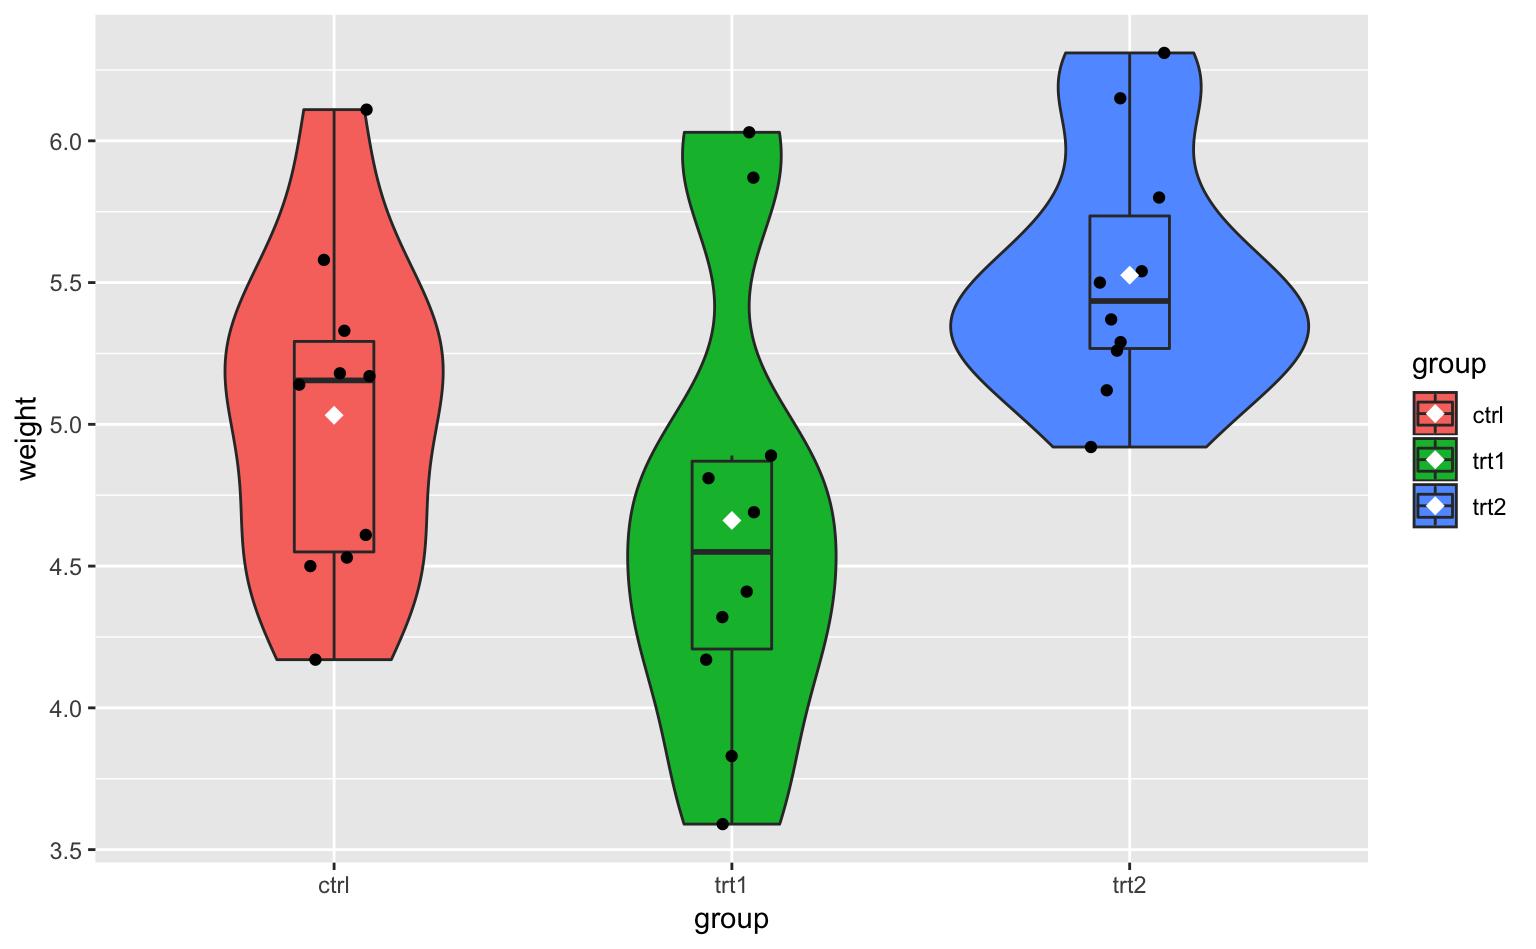
\includegraphics{lecture_note_files/figure-latex/unnamed-chunk-44-1} 

}

\caption{(ref:strip-plot)}\label{fig:unnamed-chunk-44}
\end{figure}

図中の黒いドットたちがストリッププロットである。1個1個のドットはデータそのものを表している。

コードの内容を上から順に解説する。

\begin{enumerate}
\def\labelenumi{\arabic{enumi}.}
\setcounter{enumi}{-1}
\item
  \texttt{ggplot(PlantGrowth,\ aes(group,\ weight,\ fill\ =\ group))}

  \begin{itemize}
  \tightlist
  \item
    x軸に\texttt{group}、y軸に\texttt{weight}を指定。\texttt{group}ごとに塗りつぶす。
  \end{itemize}
\item
  \texttt{geom\_violin()}

  \begin{itemize}
  \tightlist
  \item
    バイオリンプロットを描く。
  \end{itemize}
\item
  \texttt{geom\_boxplot(outlier.shape\ =\ NA,\ width\ =\ 0.2)}

  \begin{itemize}
  \item
    その上に箱ひげ図を描く。
  \item
    \texttt{outlier.shape\ =\ NA}として外れ値を消すのがポイント。デフォルトだと、箱ひげ図の外れ値とストリッププロットのドットが混在してしまう。
  \item
    \texttt{width}は箱ひげ図の幅を調整する引数。1がデフォルトの大きさ。
  \end{itemize}
\item
  \texttt{geom\_point(position\ =\ position\_jitter(width\ =\ 0.1,\ seed\ =\ 1))}

  \begin{itemize}
  \item
    さらにストリッププロット(ドット)を描く。
  \item
    \texttt{position\ =\ position\_jitter()}はドットの位置をジッター(jitter:散らばらせる)ための関数である。これを設定しないと、ドットが縦一列に並んでしまい、データ構造が非常に見づらくなる(気になる人は、試しに\texttt{position}以下を消して実行してみよう)。
  \item
    \texttt{width}は水平(x軸)方向の散らばり幅を調整する引数。また、\texttt{seed}はジッター具合を決めるための引数(乱数生成のシード)である。これを決めないと毎回ドットの位置が変わってしまうので、再現性を担保するためにも設定しておくと良い(気になる人は、試しに\texttt{seed}以下を消した上で何回か実行してみよう)。
  \item
    この図の場合、ドットが垂直(y軸)方向にも散らばっていると、誤解を招く結果を導きかねない。そのため、\texttt{height}(垂直方向の散らばりの大きさ)は0にしている。
  \end{itemize}
\item
  \texttt{stat\_summary(geom\ =\ "point",\ fun.y\ =\ mean,\ shape\ =\ "diamond",\ color\ =\ "white",\ size\ =\ 3)}

  \begin{itemize}
  \tightlist
  \item
    おまけに平均値を描く。
  \end{itemize}
\end{enumerate}

データポイントがそこまで大量でない場合は、このようにプロットするのが良いだろう。

\section{練習問題}\label{-1}

\begin{itemize}
\item
  Rにデフォルトで入っている\texttt{iris}(アヤメに関するデータセット\footnote{様々なデータ分析においてチュートリアル的に用いられる代表的なデータセット。\url{https://en.wikipedia.org/wiki/Iris_flower_data_set}}
  )を使い、\texttt{Species}ごとに\texttt{Sepal.Length}のヒストグラムと密度プロットをそれぞれ描いてみよう。
\item
  \texttt{Species}ごとに\texttt{Sepal.Width}の箱ひげ図、バイオリンプロット、ストリッププロットを重ね書きしてみよう。
\end{itemize}

\chapter{連続変数間の関係}\label{association}

連続変数間の関係を見たいときは、\textbf{散布図}(scatter
plot)を描くのがセオリーである。

\begin{Shaded}
\begin{Highlighting}[]
\KeywordTok{library}\NormalTok{(ggplot2) }\CommentTok{# 忘れずにパッケージを読み込む}
\end{Highlighting}
\end{Shaded}

\section{基本の散布図}

ここでは、Rにデフォルトで入っている\texttt{faithful}(オールド・フェイスフル・ガイザーに関するデータセット)を使ってみよう。ちなみに、オールド・フェイスフル・ガイザーとは、イエローストーン国立公園内にある間欠泉のことである\footnote{\url{https://ja.wikipedia.org/wiki/オールド・フェイスフル・ガイザー}}。

\begin{Shaded}
\begin{Highlighting}[]
\KeywordTok{head}\NormalTok{(faithful) }\CommentTok{# 先頭6行}
\end{Highlighting}
\end{Shaded}

\begin{verbatim}
##   eruptions waiting
## 1     3.600      79
## 2     1.800      54
## 3     3.333      74
## 4     2.283      62
## 5     4.533      85
## 6     2.883      55
\end{verbatim}

変数はそれぞれ、

\begin{itemize}
\item
  \texttt{eruptions}:間欠泉の噴出時間(分)
\item
  \texttt{waiting}:次の間欠泉が噴出するまでの時間(分)
\end{itemize}

を表している。散布図はドットから構成されるグラフなので、\texttt{geom\_point()}で描くことができる。

(ref:scatter-plot-1)
\texttt{faithful}データの散布図。強い正の相関が見て取れる。また、データを2つのクラスタに分けられそうなことが見て取れる。

\begin{Shaded}
\begin{Highlighting}[]
\KeywordTok{ggplot}\NormalTok{(faithful, }\KeywordTok{aes}\NormalTok{(eruptions, waiting)) }\OperatorTok{+}\StringTok{ }\CommentTok{# x軸にeruptions、y軸にwaiting}
\StringTok{  }\KeywordTok{geom_point}\NormalTok{() }\CommentTok{# 散布図を描く(データをドットとして表示する)}
\end{Highlighting}
\end{Shaded}

\begin{figure}

{\centering 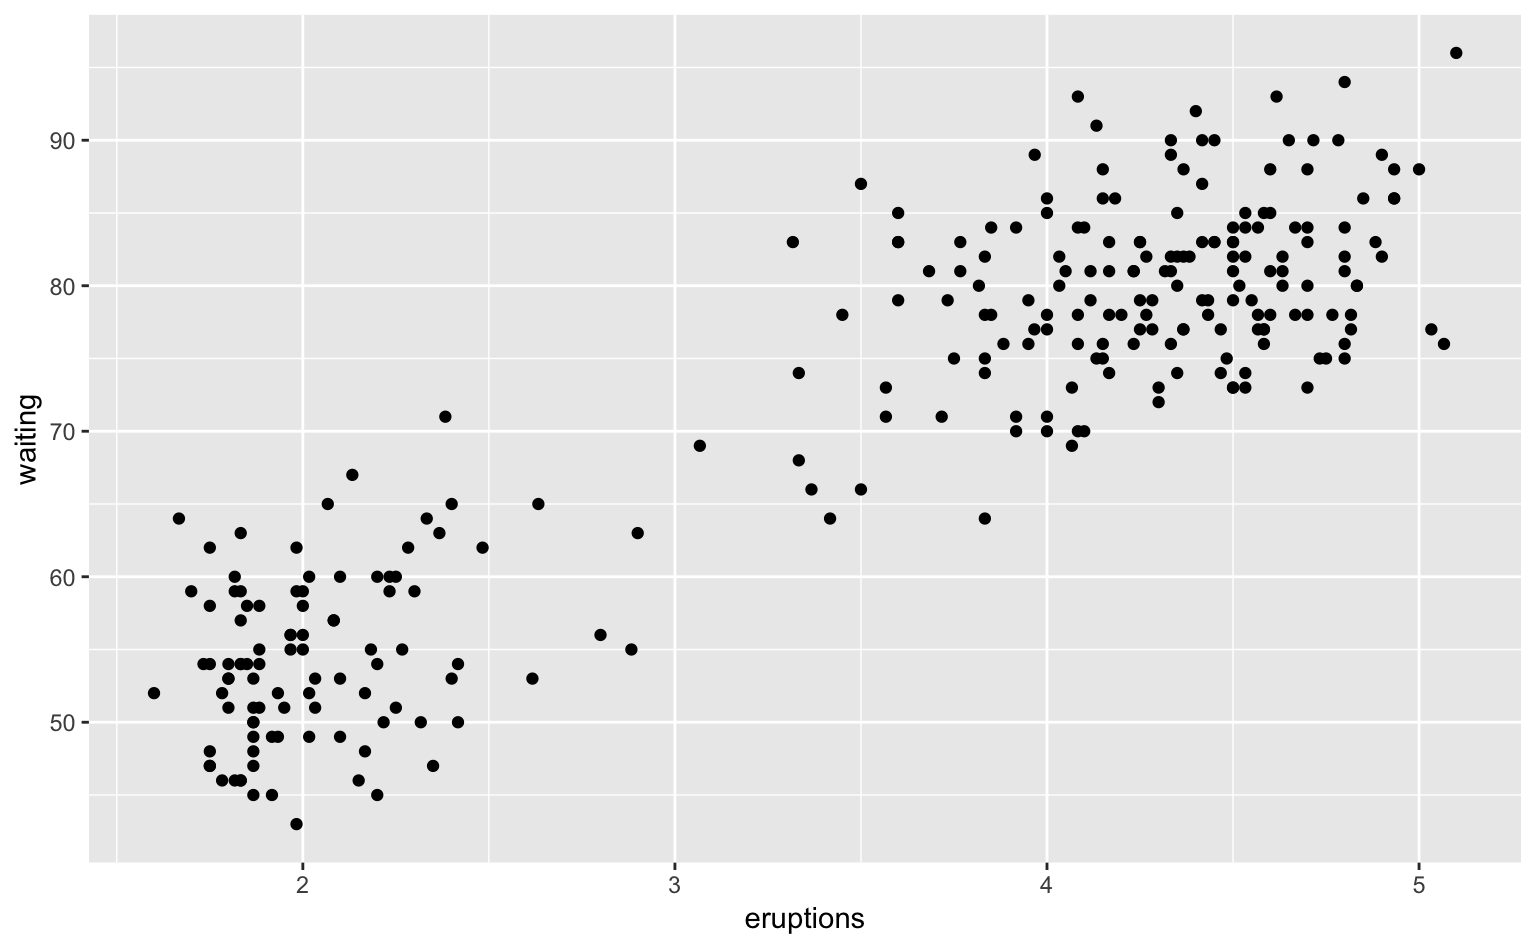
\includegraphics{lecture_note_files/figure-latex/unnamed-chunk-51-1} 

}

\caption{(ref:scatter-plot-1)}\label{fig:unnamed-chunk-51}
\end{figure}

\section{グルーピングされた散布図}

Chapter
\ref{tutorial}のチュートリアルでも見たが、複数グループの散布図を描く(グルーピングする)ことも可能である。Rにデフォルトで入っている\texttt{mtcars}を使い、改めてChapter
\ref{tutorial}で描いた散布図の復習をしよう。\texttt{geom\_point()}でグループごとに色を変えるには、\texttt{color}に変数を指定すれば良い。



\begin{Shaded}
\begin{Highlighting}[]
\KeywordTok{ggplot}\NormalTok{(mtcars, }\KeywordTok{aes}\NormalTok{(wt, mpg, }\DataTypeTok{color =} \KeywordTok{factor}\NormalTok{(cyl))) }\OperatorTok{+}\StringTok{ }\CommentTok{# factor(変数)とすることで、離散変数として扱える}
\StringTok{  }\KeywordTok{geom_point}\NormalTok{()}
\end{Highlighting}
\end{Shaded}

\begin{figure}

{\centering 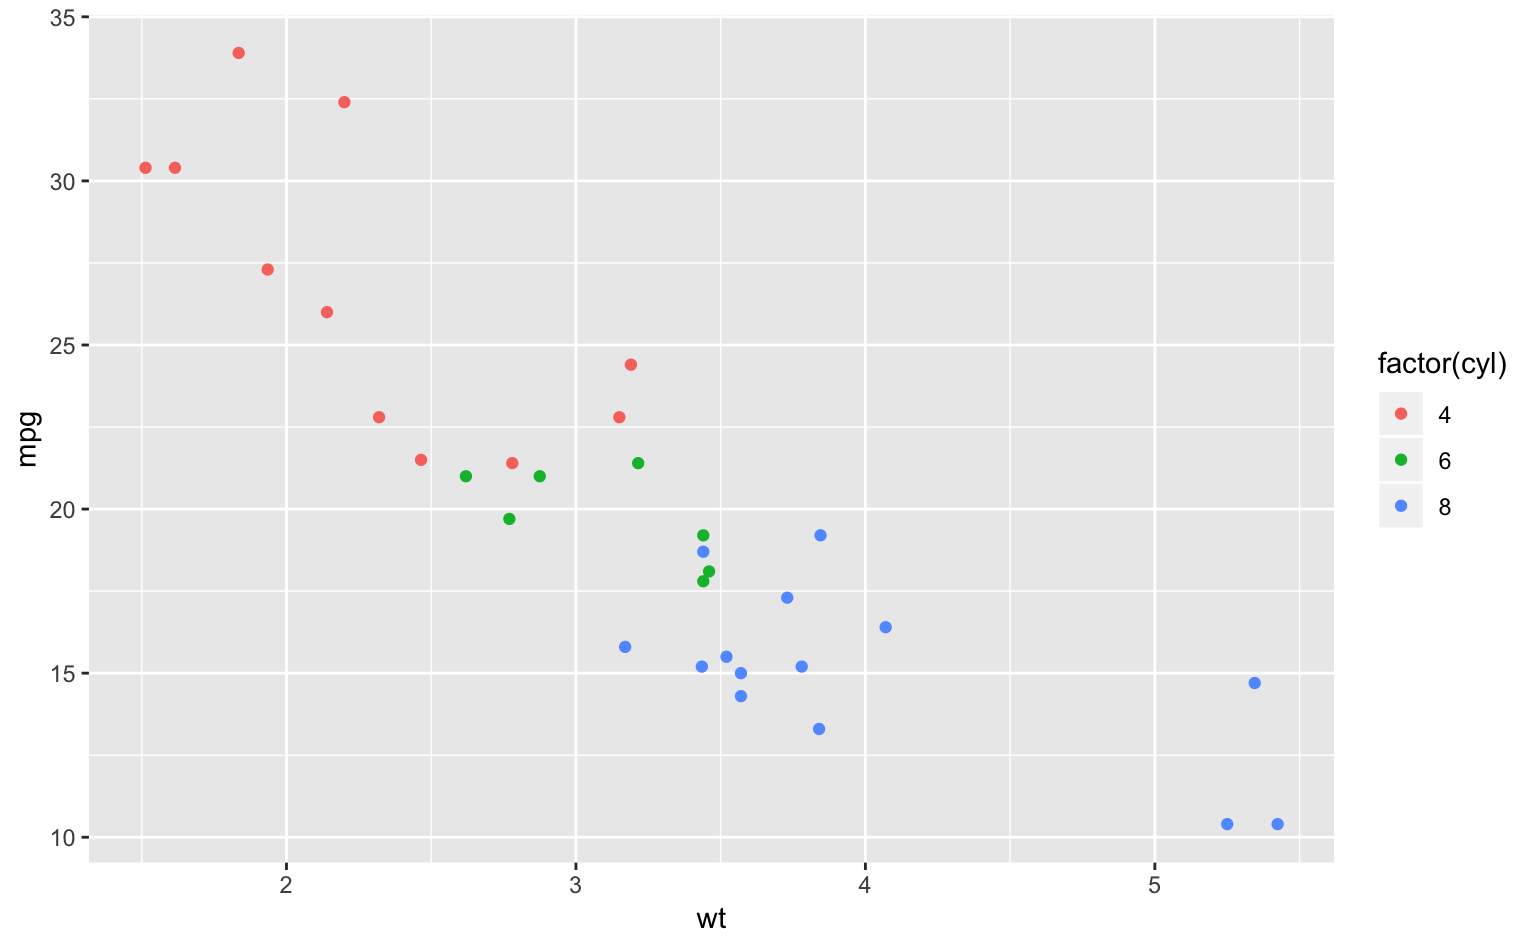
\includegraphics{lecture_note_files/figure-latex/scatter-plot-2-1} 

}

\caption{グルーピングされた散布図。}\label{fig:scatter-plot-2}
\end{figure}

見やすさや色覚バリアフリーという観点に立てば、点の形も変えたほうが良いだろう\footnote{このように、あえて情報に\textbf{冗長性}を持たせることをredundant
  codingという。}。ドットの形を変えるには、\texttt{shape}に変数を指定すれば良い。




\begin{Shaded}
\begin{Highlighting}[]
\KeywordTok{ggplot}\NormalTok{(mtcars, }\KeywordTok{aes}\NormalTok{(disp, mpg, }\DataTypeTok{color =} \KeywordTok{factor}\NormalTok{(cyl), }\DataTypeTok{shape =} \KeywordTok{factor}\NormalTok{(cyl))) }\OperatorTok{+}\StringTok{ }\CommentTok{# shape = factor(cyl)を追加}
\StringTok{  }\KeywordTok{geom_point}\NormalTok{()}
\end{Highlighting}
\end{Shaded}

\begin{figure}

{\centering 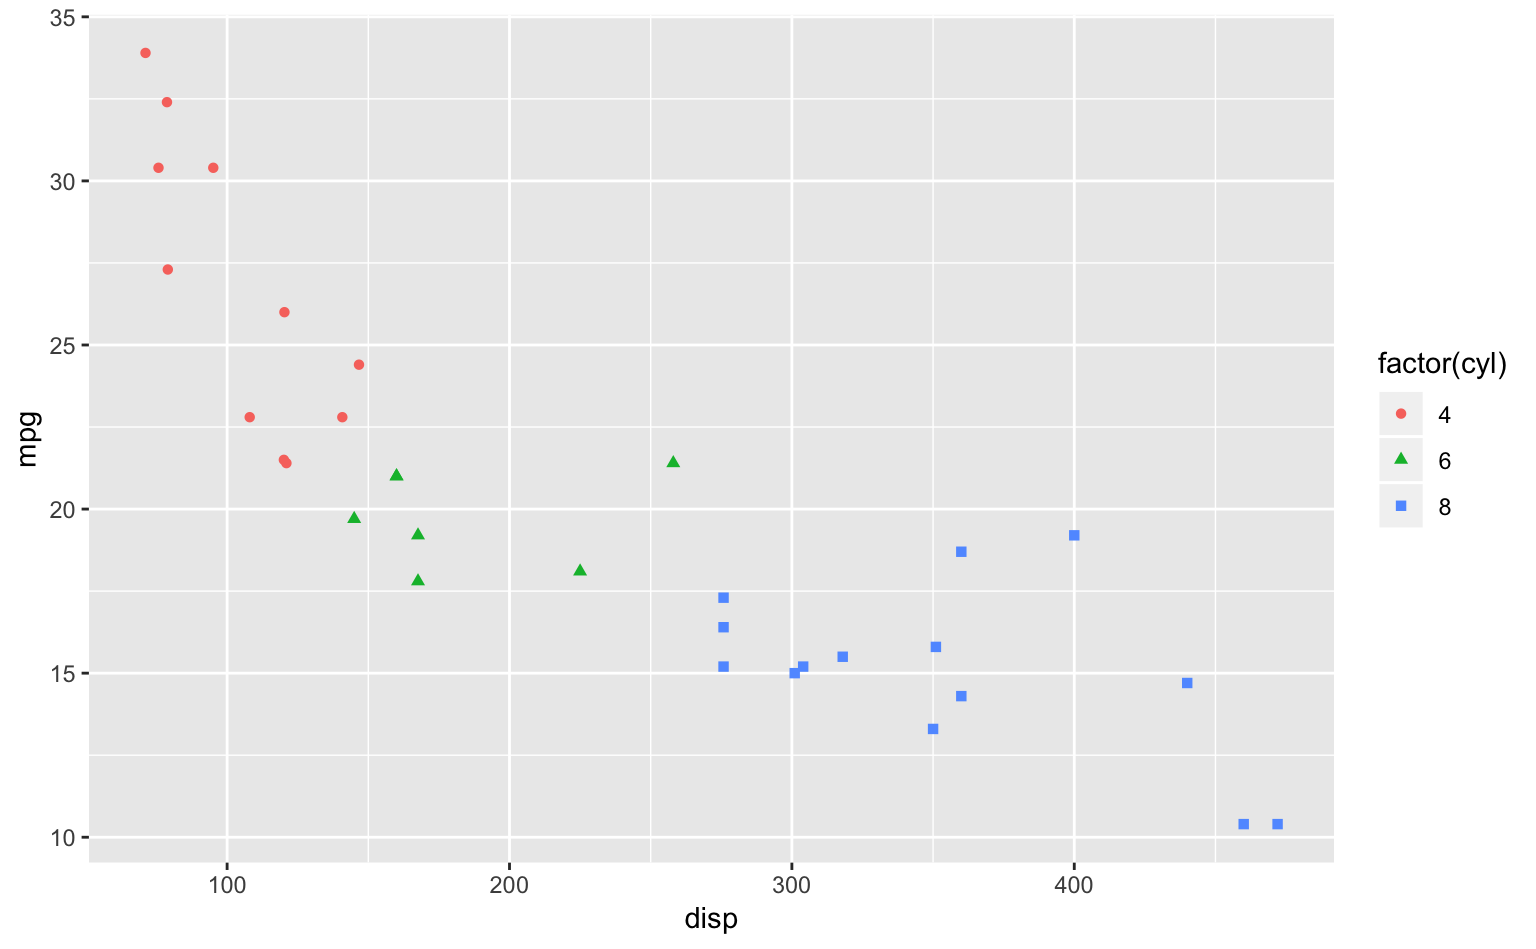
\includegraphics{lecture_note_files/figure-latex/unnamed-chunk-52-1} 

}

\caption{Figure
\ref{fig:scatter-plot-2}のドットの形を変えた散布図。}\label{fig:unnamed-chunk-52}
\end{figure}

\texttt{cyl}(シリンダーの個数)の値に応じてデータポイントの形が変わっているのが見て取れる。

\section{散布図行列}

\texttt{faithful}データは変数が2つだけなので、散布図を1つ描けば終わりである。しかし、実際のデータには多くの変数がある。変数が増えるにつれて、確認しなければならない散布図の数は爆発的に増える。そのようなとき、1つ1つ散布図を描くのは面倒である。

しかし、そんなときに便利なものがある\footnote{データ分析で「困ったなあ」とか「こういうのあれば便利なんだけど」と思うようなことは、大体海外の偉い人が既に解決してくれているものなので、困ったときはやはり(英語で)ググルに限る。これは重要なライフハックである。}。それは、GGallyパッケージの\texttt{ggpairs()}という関数である。では早速、Rにデフォルトで入っている\texttt{iris}データで試してみよう。まずはGGallyパッケージを読み込む。

\begin{Shaded}
\begin{Highlighting}[]
\KeywordTok{library}\NormalTok{(GGally) }\CommentTok{# パッケージの読み込み}
\end{Highlighting}
\end{Shaded}

あとは、\texttt{ggpairs()}にデータセットを突っ込むだけ。以上。

(ref:scatter-plot-matrix-1)
\texttt{ggpairs()}による\texttt{iris}データの散布図行列。散布図だけでなく、変数の種類に応じて自動で箱ひげ図などもプロットされる。

\begin{Shaded}
\begin{Highlighting}[]
\KeywordTok{ggpairs}\NormalTok{(iris) }\CommentTok{# 散布図行列を描く}
\end{Highlighting}
\end{Shaded}

\begin{figure}

{\centering 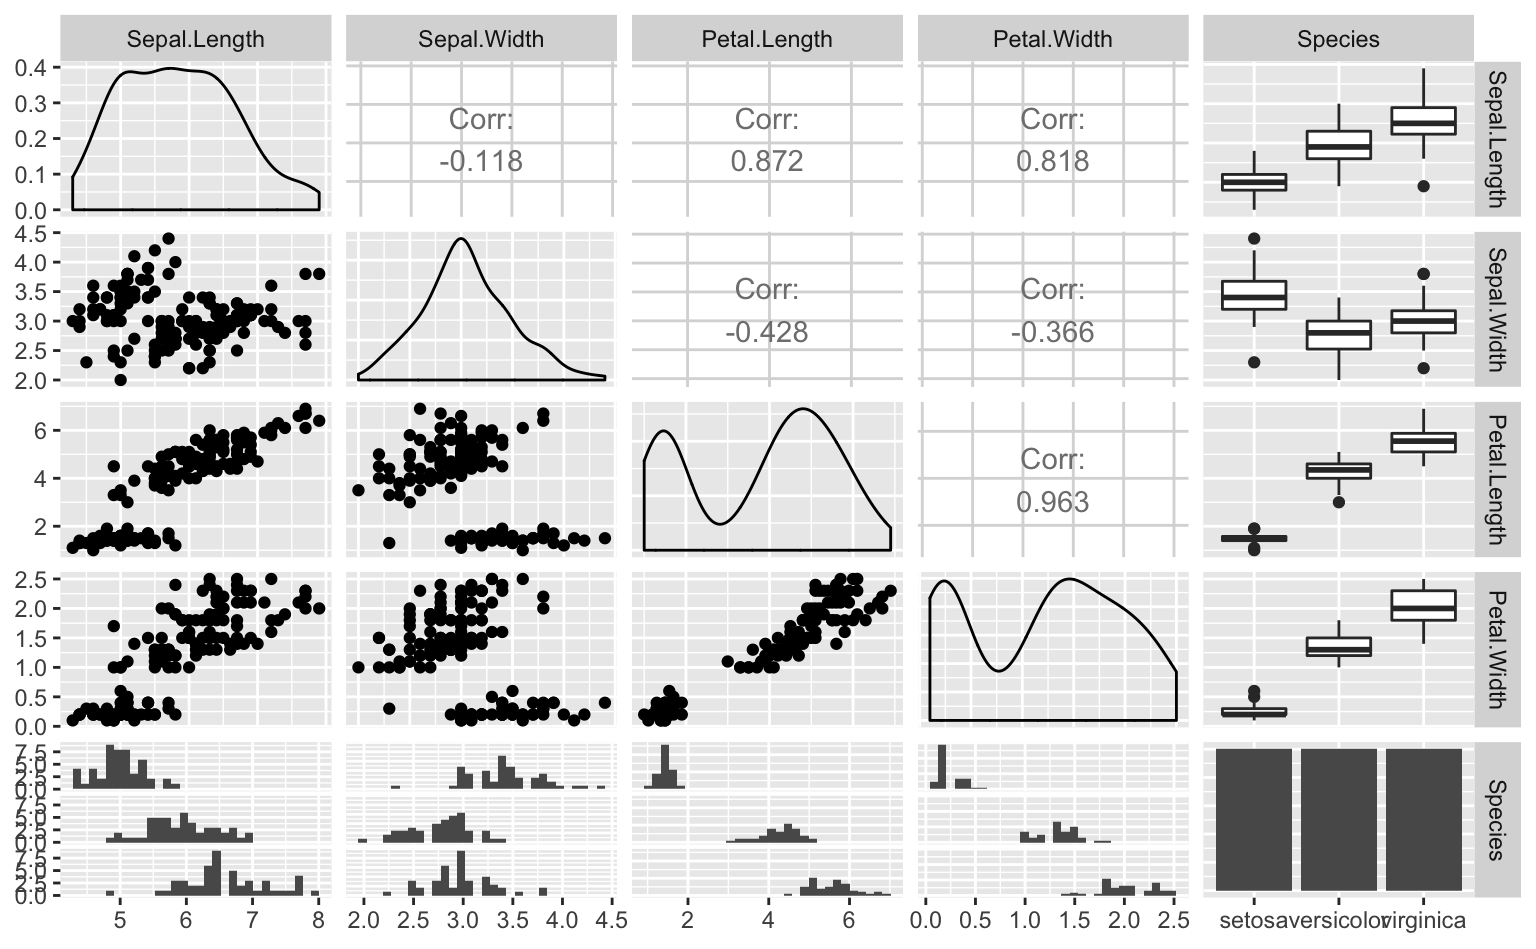
\includegraphics{lecture_note_files/figure-latex/scatter-plot-matrix-1-1} 

}

\caption{(ref:scatter-plot-matrix-1)}\label{fig:scatter-plot-matrix-1}
\end{figure}

なんと、これだけで多変量の散布図、箱ひげ図などを一撃で描画できてしまうのである。しかも、変数の連続/離散に応じて適切なグラフを選んでくれる親切ゆとり設計である。

ただ、これだけでは少し味気ないので、\texttt{Species}に応じて色をつけてみよう。ggplot2と同じように指定すれば良い。




\begin{Shaded}
\begin{Highlighting}[]
\KeywordTok{ggpairs}\NormalTok{(iris, }\KeywordTok{aes}\NormalTok{(}\DataTypeTok{color =}\NormalTok{ Species, }\DataTypeTok{alpha =} \FloatTok{0.7}\NormalTok{)) }\CommentTok{# ggplot2と同じように色と透明度を指定}
\end{Highlighting}
\end{Shaded}

\begin{figure}

{\centering 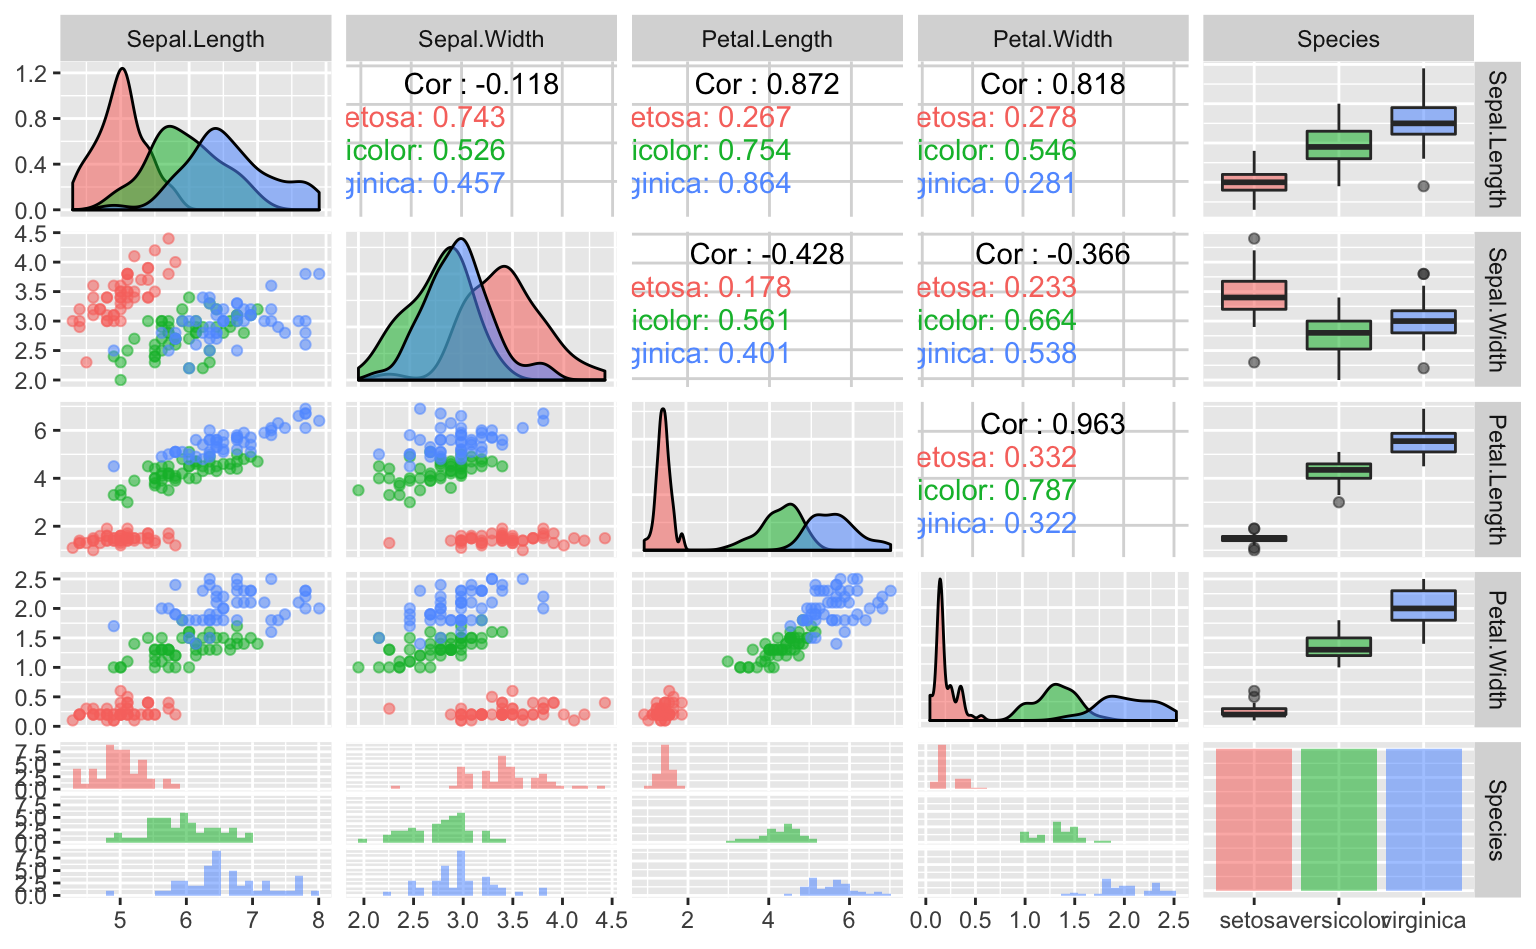
\includegraphics{lecture_note_files/figure-latex/unnamed-chunk-54-1} 

}

\caption{Figure
\ref{fig:scatter-plot-matrix-1}に色をつけて半透明にした図。}\label{fig:unnamed-chunk-54}
\end{figure}

他にも細かい設定ができるそうだが、ここでは説明を割愛する\footnote{ぶっちゃけあまり知らない。}。

\section{オーバープロットへの対処}

最後に、オーバープロットというものへの対処法を見ていくことにする。具体例として、ggplot2に入っている\texttt{mpg}データを使ってみよう。

\begin{Shaded}
\begin{Highlighting}[]
\KeywordTok{head}\NormalTok{(mpg) }\CommentTok{# 先頭6行}
\end{Highlighting}
\end{Shaded}

\begin{verbatim}
## # A tibble: 6 x 11
##   manufacturer model displ  year   cyl trans      drv     cty   hwy fl   
##   <chr>        <chr> <dbl> <int> <int> <chr>      <chr> <int> <int> <chr>
## 1 audi         a4      1.8  1999     4 auto(l5)   f        18    29 p    
## 2 audi         a4      1.8  1999     4 manual(m5) f        21    29 p    
## 3 audi         a4      2    2008     4 manual(m6) f        20    31 p    
## 4 audi         a4      2    2008     4 auto(av)   f        21    30 p    
## 5 audi         a4      2.8  1999     6 auto(l5)   f        16    26 p    
## 6 audi         a4      2.8  1999     6 manual(m5) f        18    26 p    
##   class  
##   <chr>  
## 1 compact
## 2 compact
## 3 compact
## 4 compact
## 5 compact
## 6 compact
\end{verbatim}

注目する変数は、

\begin{itemize}
\item
  \texttt{displ}:エンジンの排気量(リットル)
\item
  \texttt{hwy}:燃費(マイル/ガロン)
\item
  \texttt{cyl}:シリンダー数(4, 5, 6, or 8)
\end{itemize}

の3つである。早速、\texttt{x}に\texttt{displ}、\texttt{y}に\texttt{hwy}、\texttt{color}に\texttt{factor(cyl)}を指定して散布図を描いてみよう。



\begin{Shaded}
\begin{Highlighting}[]
\KeywordTok{ggplot}\NormalTok{(mpg, }\KeywordTok{aes}\NormalTok{(displ, hwy, }\DataTypeTok{color =} \KeywordTok{factor}\NormalTok{(cyl))) }\OperatorTok{+}
\StringTok{  }\KeywordTok{geom_point}\NormalTok{()}
\end{Highlighting}
\end{Shaded}

\begin{figure}

{\centering 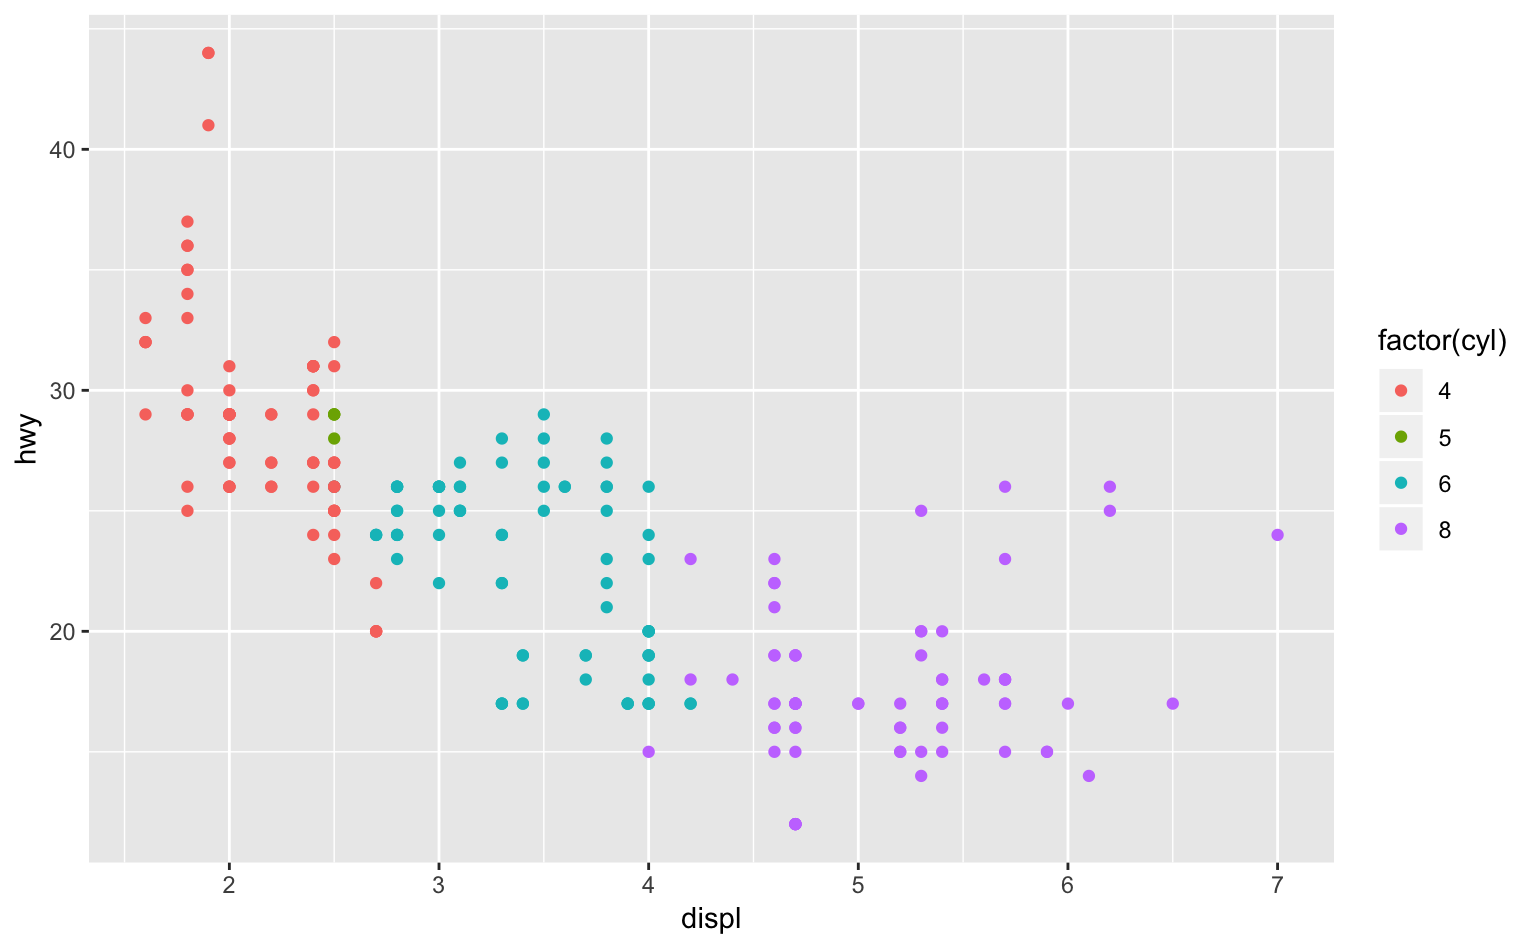
\includegraphics{lecture_note_files/figure-latex/scatter-plot-4-1} 

}

\caption{デフォルトの設定で描いた散布図。}\label{fig:scatter-plot-4}
\end{figure}

とりあえず散布図を描くことができた。一見問題は無さそうである。

では、ここで\texttt{mpg}のデータの行数(データポイントの数)を確認してみよう。\texttt{nrow(データセット)}で確認することができる。

\begin{Shaded}
\begin{Highlighting}[]
\KeywordTok{nrow}\NormalTok{(mpg)}
\end{Highlighting}
\end{Shaded}

\begin{verbatim}
## [1] 234
\end{verbatim}

なんと234個もあった。しかし、Figure
\ref{fig:scatter-plot-4}の散布図では、データ(ドット)がせいぜい数十〜百個ぐらいにしか見えない。なぜだろうか?

なぜなら、x軸の値とy軸の値が全く同じデータポイントが複数個存在しており、それらが重なってしまっているからである。このような状態を\textbf{オーバープロット}(overplotting)という。

たとえば、7件法のリカート尺度によって実験参加者の特性を測り、その散布図を描くというときに、オーバープロットは間違いなく生じる。では、どのように対処すればよいのだろうか? ここでは、Chapter
\ref{distribution}でも扱ったジッター(jittering)というテクニックを使えば良い。



\begin{Shaded}
\begin{Highlighting}[]
\KeywordTok{ggplot}\NormalTok{(mpg, }\KeywordTok{aes}\NormalTok{(displ, hwy, }\DataTypeTok{color =} \KeywordTok{factor}\NormalTok{(cyl))) }\OperatorTok{+}
\StringTok{  }\KeywordTok{geom_point}\NormalTok{(}\DataTypeTok{position =} \KeywordTok{position_jitter}\NormalTok{(}\DataTypeTok{width =} \FloatTok{0.1}\NormalTok{, }\DataTypeTok{height =} \FloatTok{0.4}\NormalTok{, }\DataTypeTok{seed =} \DecValTok{1}\NormalTok{)) }\CommentTok{# ドットをジッターさせている}
\end{Highlighting}
\end{Shaded}

\begin{figure}

{\centering 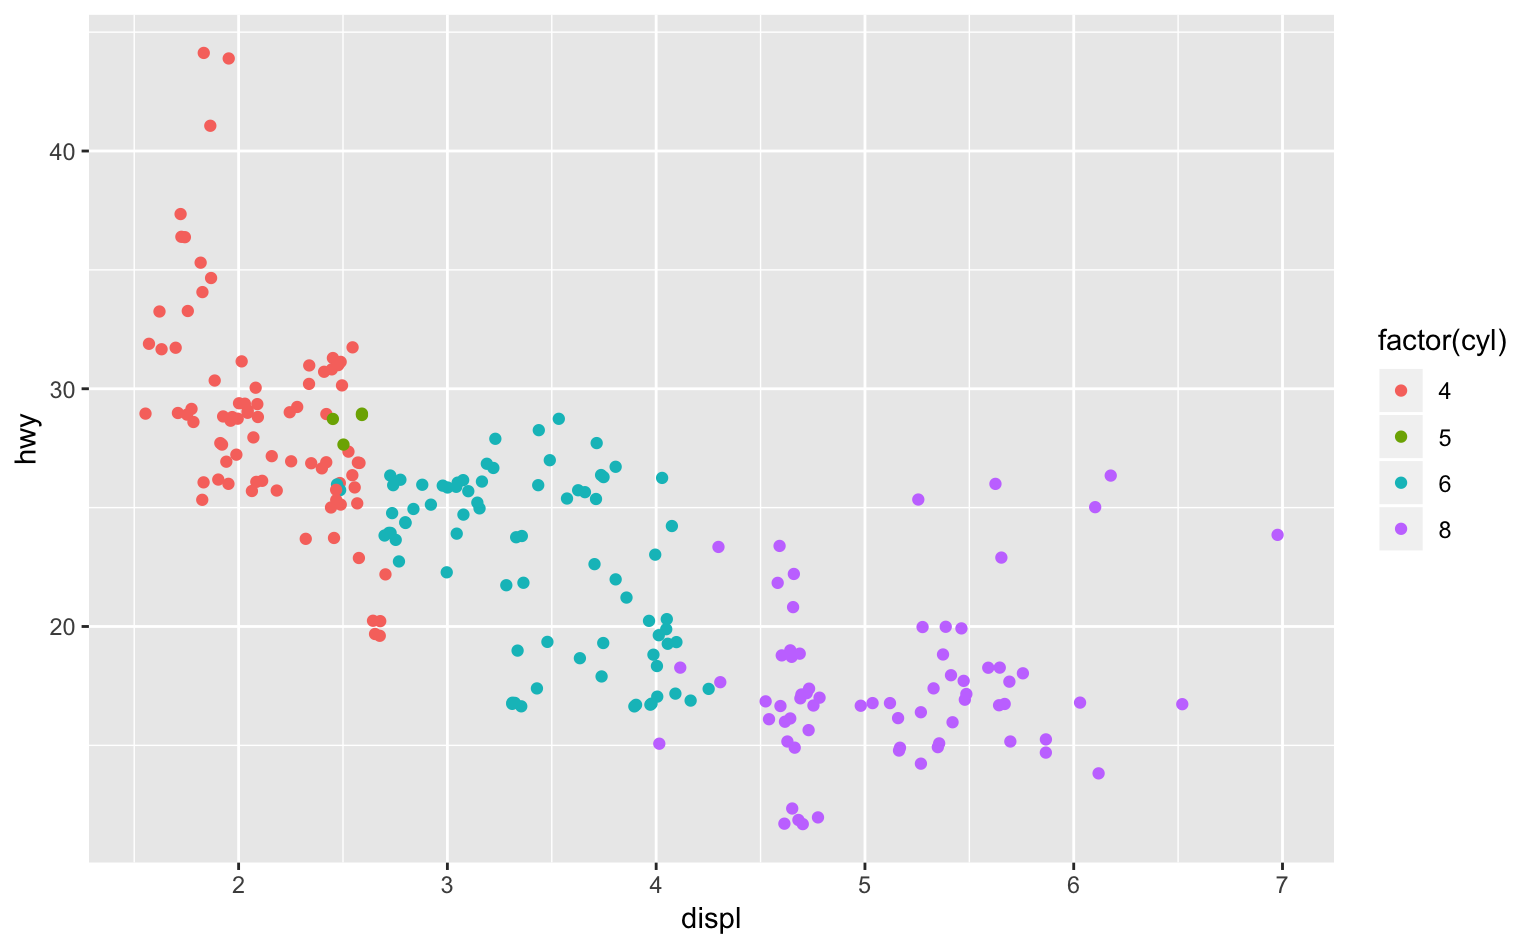
\includegraphics{lecture_note_files/figure-latex/scatter-plot-5-1} 

}

\caption{ドットをジッターさせた散布図。}\label{fig:scatter-plot-5}
\end{figure}

\texttt{position\ =\ position\_jitter(width\ =\ ...,\ height\ =\ ...,\ seed\ =\ ...)}を指定することで、オーバープロットを回避することができた。このとき、\texttt{width}や\texttt{height}に大きすぎる値を入れてしまうと、データが大きく歪んでしまうので注意が必要である。

また、ここで点の形状や透明度を調節すれば、重複している箇所がより見やすくなって良いだろう。




\begin{Shaded}
\begin{Highlighting}[]
\KeywordTok{ggplot}\NormalTok{(mpg, }\KeywordTok{aes}\NormalTok{(displ, hwy, }\DataTypeTok{color =} \KeywordTok{factor}\NormalTok{(cyl), }\DataTypeTok{shape =} \KeywordTok{factor}\NormalTok{(cyl))) }\OperatorTok{+}\StringTok{ }\CommentTok{# shapeに変数を指定}
\StringTok{  }\KeywordTok{geom_point}\NormalTok{(}\DataTypeTok{position =} \KeywordTok{position_jitter}\NormalTok{(}\DataTypeTok{width =} \FloatTok{0.1}\NormalTok{, }\DataTypeTok{height =} \FloatTok{0.4}\NormalTok{, }\DataTypeTok{seed =} \DecValTok{1}\NormalTok{), }\DataTypeTok{alpha =} \FloatTok{0.7}\NormalTok{) }\CommentTok{# alpha = 0.7を追加}
\end{Highlighting}
\end{Shaded}

\begin{figure}

{\centering 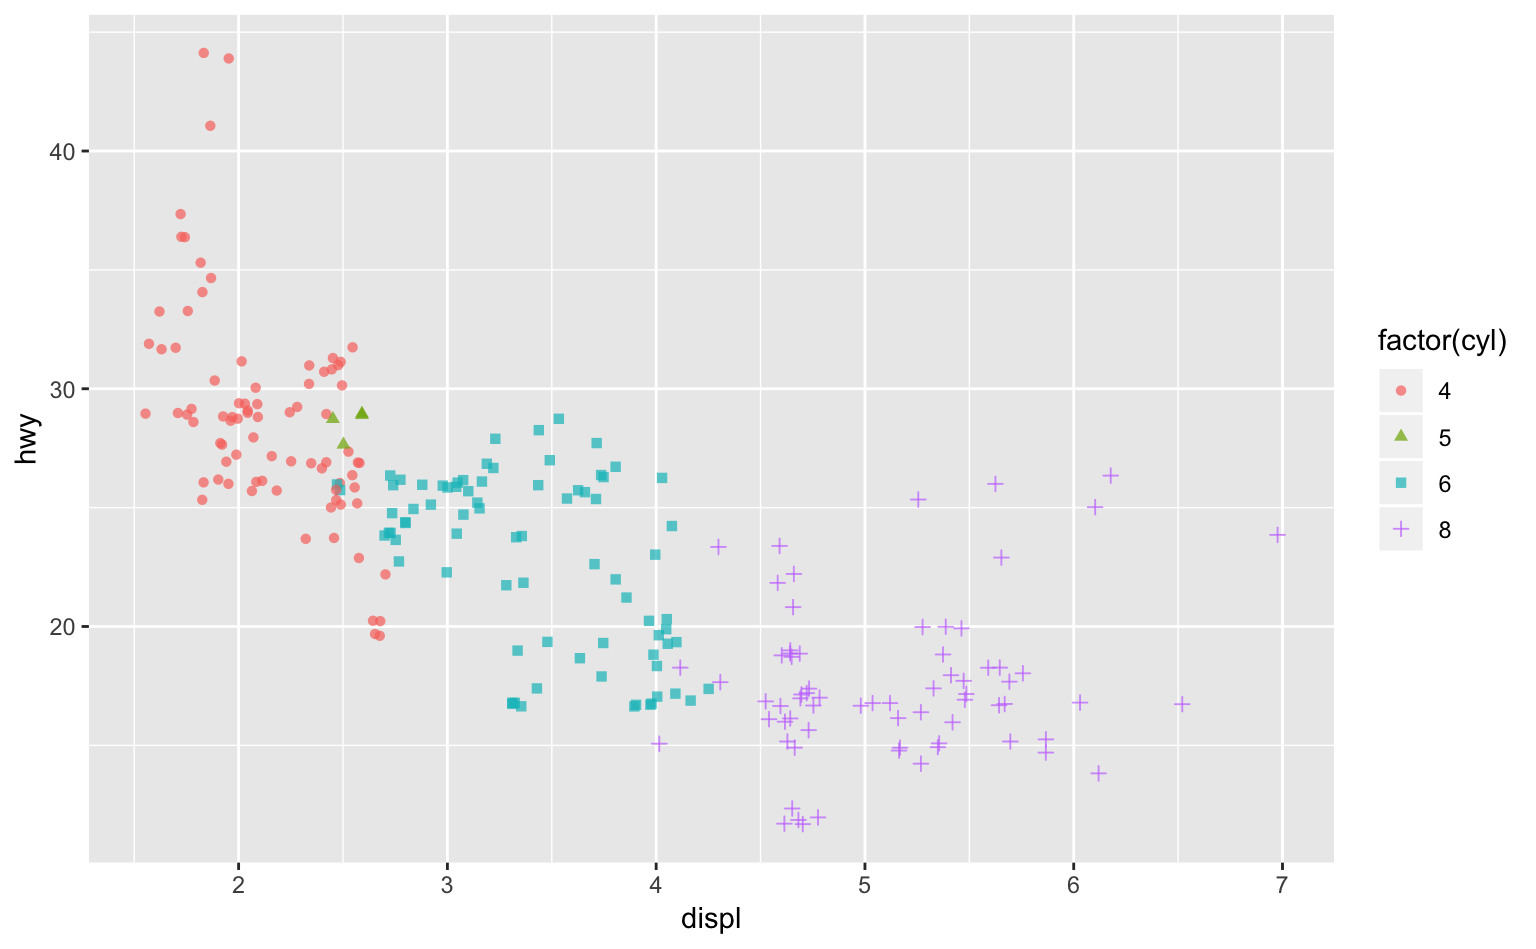
\includegraphics{lecture_note_files/figure-latex/unnamed-chunk-57-1} 

}

\caption{Figure
\ref{fig:scatter-plot-5}のドットの形状と透明度を変えたもの。}\label{fig:unnamed-chunk-57}
\end{figure}

\section{練習問題}\label{-2}

\begin{itemize}
\item
  Rにデフォルトで入っている\texttt{trees}データを使い、\texttt{Girth}と\texttt{Volume}の散布図を描いてみよう。
\item
  gcookbookの\texttt{heightweight}データの散布図行列を描いてみよう。
\end{itemize}

\chapter{トレンドデータ}\label{trend-data}

x軸が時間であったり、連続変数かつ何かしらの説明要因である場合、\textbf{折れ線グラフ}(line
graph)を描くのがセオリーである。

\begin{Shaded}
\begin{Highlighting}[]
\KeywordTok{library}\NormalTok{(ggplot2) }\CommentTok{# 忘れずにパッケージを読み込む}
\end{Highlighting}
\end{Shaded}

\section{基本の折れ線グラフ}

まずは、gcookbookの\texttt{aapl}データ(Appleの週ごとの株価データ)を可視化してみよう。

\begin{Shaded}
\begin{Highlighting}[]
\KeywordTok{library}\NormalTok{(gcookbook) }\CommentTok{# パッケージの読み込み}
\end{Highlighting}
\end{Shaded}

\begin{Shaded}
\begin{Highlighting}[]
\KeywordTok{head}\NormalTok{(aapl) }\CommentTok{# 先頭6行}
\end{Highlighting}
\end{Shaded}

\begin{verbatim}
##         date adj_price
## 1 1980-12-12  0.023268
## 2 1980-12-19  0.022863
## 3 1980-12-26  0.028731
## 4 1981-01-02  0.027921
## 5 1981-01-09  0.025797
## 6 1981-01-16  0.025089
\end{verbatim}

変数はそれぞれ、

\begin{itemize}
\item
  \texttt{date}:記録日
\item
  \texttt{adj\_price}:株価
\end{itemize}

を表している。では、株価の時系列変化をプロットしてみよう。\texttt{geom\_line()}で折れ線グラフを描くことができる。



\begin{Shaded}
\begin{Highlighting}[]
\KeywordTok{ggplot}\NormalTok{(aapl, }\KeywordTok{aes}\NormalTok{(date, adj_price)) }\OperatorTok{+}\StringTok{ }\CommentTok{# x軸にdate、y軸にadj_price}
\StringTok{  }\KeywordTok{geom_line}\NormalTok{() }\CommentTok{# 折れ線グラフ}
\end{Highlighting}
\end{Shaded}

\begin{figure}

{\centering 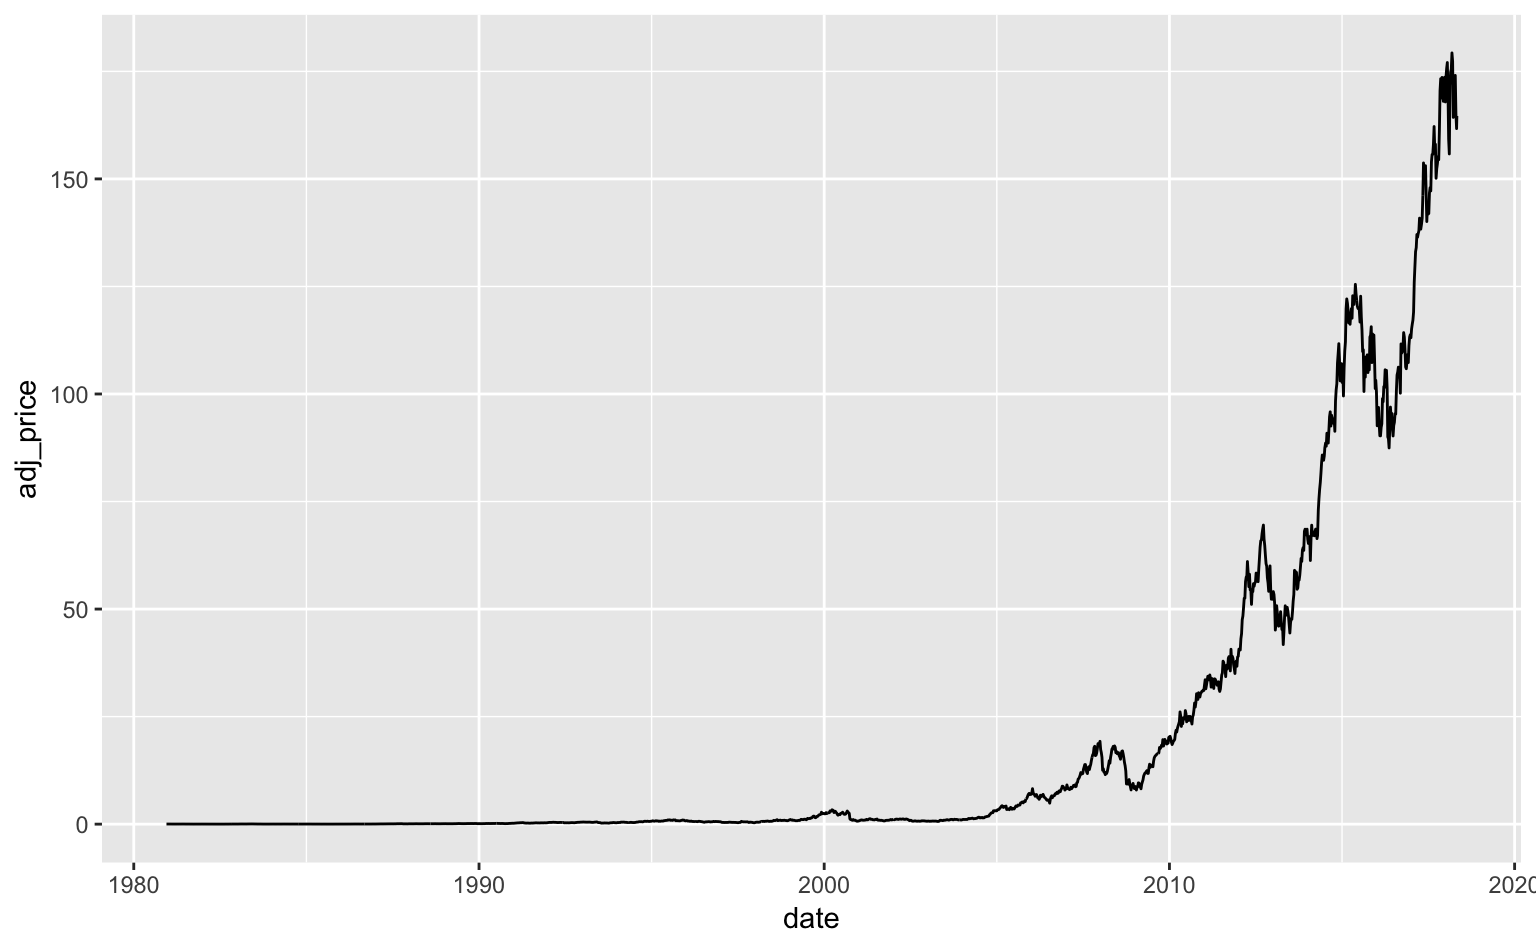
\includegraphics{lecture_note_files/figure-latex/line-graph-1-1} 

}

\caption{Appleの株価データ。}\label{fig:line-graph-1}
\end{figure}

\begin{center}\rule{0.5\linewidth}{\linethickness}\end{center}

次は、Rにデフォルトで入っている\texttt{BOD}(生物化学的酸素要求量に関するデータセット)を可視化してみよう。なお、生物化学的酸素要求量(biochemical
oxygen demand; BOD)とは水質指標のことである\footnote{\url{https://ja.wikipedia.org/wiki/生物化学的酸素要求量}}。

\begin{Shaded}
\begin{Highlighting}[]
\KeywordTok{head}\NormalTok{(BOD) }\CommentTok{# 6行しかないのですべて表示される}
\end{Highlighting}
\end{Shaded}

\begin{verbatim}
##   Time demand
## 1    1    8.3
## 2    2   10.3
## 3    3   19.0
## 4    4   16.0
## 5    5   15.6
## 6    7   19.8
\end{verbatim}

早速、\texttt{x}に\texttt{Time}(時間)、\texttt{y}に\texttt{Demand}(BOD)を取って折れ線グラフを描いてみよう。



\begin{Shaded}
\begin{Highlighting}[]
\KeywordTok{ggplot}\NormalTok{(BOD, }\KeywordTok{aes}\NormalTok{(Time, demand)) }\OperatorTok{+}\StringTok{ }\CommentTok{# x軸にTime、y軸にdemand}
\StringTok{  }\KeywordTok{geom_line}\NormalTok{() }\OperatorTok{+}\StringTok{ }\CommentTok{# 折れ線グラフ}
\StringTok{  }\KeywordTok{geom_point}\NormalTok{() }\CommentTok{# ドットは添えるだけ}
\end{Highlighting}
\end{Shaded}

\begin{figure}

{\centering 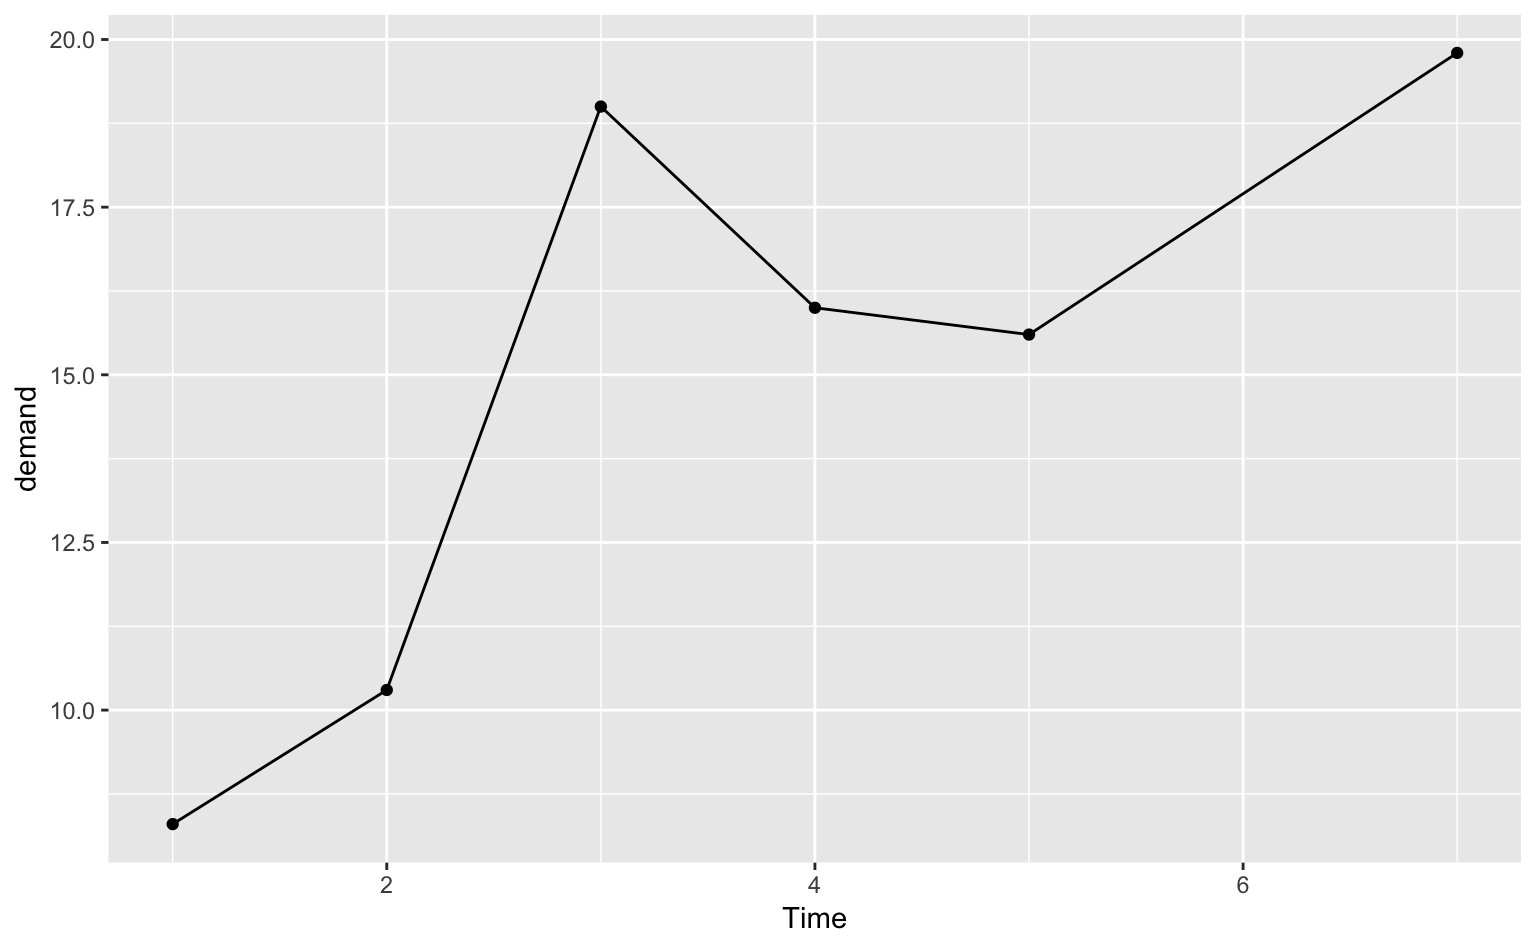
\includegraphics{lecture_note_files/figure-latex/unnamed-chunk-65-1} 

}

\caption{BODの折れ線グラフ。}\label{fig:unnamed-chunk-65}
\end{figure}

なお、ここでは\texttt{geom\_point()}を加えることで、ドットもプロットしている。\texttt{BOD}のようにデータポイントが少ない場合、折れ線だけでなく、ドットを添えると視覚的に楽になるように思われる(個人的意見だが)。逆に、Figure
\ref{fig:line-graph-1}のようにデータポイントが多い場合、ドットは不要である。

\section{グルーピングされた折れ線グラフ}

では、例のごとく、折れ線グラフを複数のグループごとに描いてみよう。ここでは、Rにデフォルトで入っている\texttt{ToothGrowth}(モルモットの歯に関するデータセット)を使ってみることにする。早速データを確認してみよう。

\begin{Shaded}
\begin{Highlighting}[]
\KeywordTok{head}\NormalTok{(ToothGrowth) }\CommentTok{# 先頭6行}
\end{Highlighting}
\end{Shaded}

\begin{verbatim}
##    len supp dose
## 1  4.2   VC  0.5
## 2 11.5   VC  0.5
## 3  7.3   VC  0.5
## 4  5.8   VC  0.5
## 5  6.4   VC  0.5
## 6 10.0   VC  0.5
\end{verbatim}

変数はそれぞれ、

\begin{itemize}
\item
  \texttt{len}:モルモットの歯の長さ
\item
  \texttt{supp}:ビタミンCの与え方(VC or
  OJ;アスコルビン酸かオレンジジュース)
\item
  \texttt{dose}:ビタミンCの投与量(mg/日)
\end{itemize}

を表している。ここで、\texttt{supp}と\texttt{dose}ごとに\texttt{len}の平均値をプロットしてみようと思うのだが、\texttt{ToothGrowth}には平均値のデータが入っておらず、自分で計算しなくてはならない。そこで、以下のコードを使って、平均値のデータセット(\texttt{tg\_mean})を新しく作ることにする。なお、今はまだ下のコードの内容を理解できなくても良い\footnote{データハンドリングなどについては、Chapter
  \ref{data-handling}で詳しく見ることにする。}。

\begin{Shaded}
\begin{Highlighting}[]
\KeywordTok{library}\NormalTok{(tidyverse) }\CommentTok{# データ加工用のパッケージ群を読み込む。色々メッセージが出るだろうが気にしなくて良い。}
\end{Highlighting}
\end{Shaded}

\begin{Shaded}
\begin{Highlighting}[]
\NormalTok{tg_mean =}\StringTok{ }\NormalTok{ToothGrowth }\OperatorTok\StringTok{ }\CommentTok{# ToothGrowthデータの}
\StringTok{  }\KeywordTok{group_by}\NormalTok{(supp, dose) }\OperatorTok\StringTok{ }\CommentTok{# suppとdoseごとに}
\StringTok{  }\KeywordTok{summarise}\NormalTok{(}\DataTypeTok{mean =} \KeywordTok{mean}\NormalTok{(len)) }\CommentTok{# lenの平均値を計算せよ}

\NormalTok{tg_mean}
\end{Highlighting}
\end{Shaded}

\begin{verbatim}
## # A tibble: 6 x 3
## # Groups:   supp [?]
##   supp   dose  mean
##   <fct> <dbl> <dbl>
## 1 OJ      0.5 13.2 
## 2 OJ      1   22.7 
## 3 OJ      2   26.1 
## 4 VC      0.5  7.98
## 5 VC      1   16.8 
## 6 VC      2   26.1
\end{verbatim}

\texttt{mean}はモルモットの歯の長さ(\texttt{len})の平均値を表している。

それでは、以下のコードを実行して、\texttt{supp}ごとに\texttt{dose}と\texttt{mean}の関係を可視化してみよう。



\begin{Shaded}
\begin{Highlighting}[]
\KeywordTok{ggplot}\NormalTok{(tg_mean, }\KeywordTok{aes}\NormalTok{(dose, mean, }\DataTypeTok{group =}\NormalTok{ supp)) }\OperatorTok{+}\StringTok{ }\CommentTok{# x軸にdose、y軸にmean;group = suppが必要}
\StringTok{  }\KeywordTok{geom_line}\NormalTok{()}
\end{Highlighting}
\end{Shaded}

\begin{figure}

{\centering 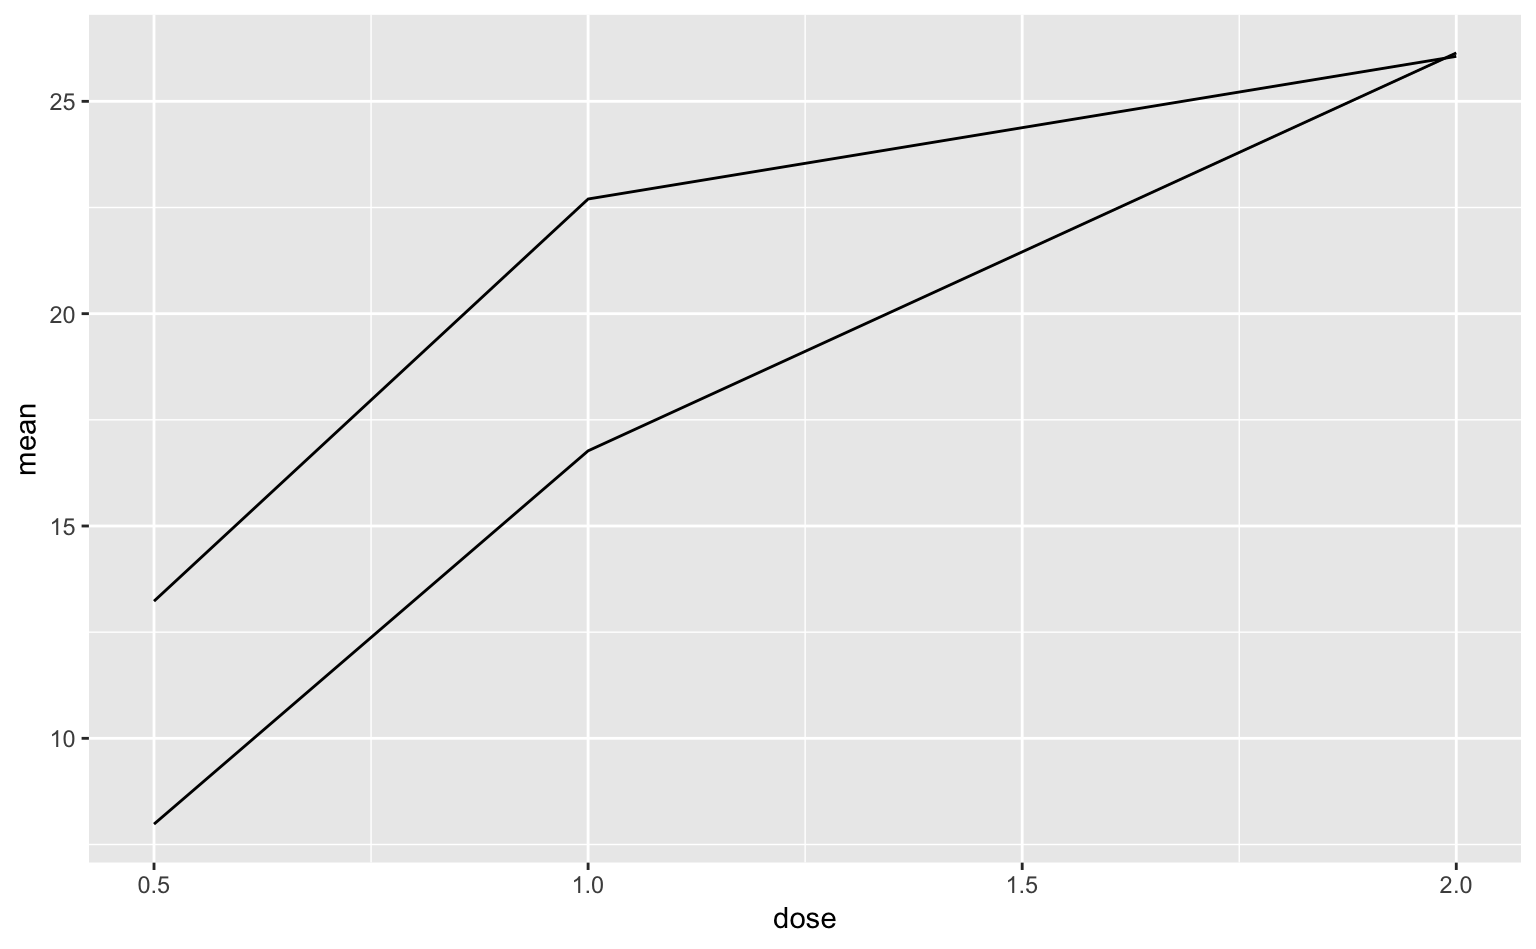
\includegraphics{lecture_note_files/figure-latex/line-graph-3-1} 

}

\caption{\texttt{supp}ごとにグルーピングされた折れ線グラフ。}\label{fig:line-graph-3}
\end{figure}

\texttt{supp}ごとに\texttt{dose}と\texttt{mean}の関係をプロットすることができた。なお、\texttt{geom\_line()}をグルーピングする際には、\texttt{group}に変数を指定しなければならない(指定しないとどうなるのだろうか? 気になる人は確認してみよう)。

ただし、このままでは見にくいので、折れ線の色(\texttt{color})と線種(\texttt{linetype})にも変数を指定しよう。また、\texttt{geom\_line()}の\texttt{size}で折れ線の太さを調整しよう。

加えて、ドットも付け足しておこう。Chapter
\ref{association}でも見たように、\texttt{shape}に変数を指定するとドットの形を変えることができる。また、\texttt{geom\_point()}の\texttt{size}でドットの大きさを調整しよう。




\begin{Shaded}
\begin{Highlighting}[]
\KeywordTok{ggplot}\NormalTok{(tg_mean, }\KeywordTok{aes}\NormalTok{(dose, mean, }\DataTypeTok{color =}\NormalTok{ supp, }\DataTypeTok{group =}\NormalTok{ supp, }\DataTypeTok{linetype =}\NormalTok{ supp, }\DataTypeTok{shape =}\NormalTok{ supp)) }\OperatorTok{+}\StringTok{ }\CommentTok{# color、linetype、shape = suppを追加}
\StringTok{  }\KeywordTok{geom_line}\NormalTok{(}\DataTypeTok{size =} \FloatTok{1.5}\NormalTok{) }\OperatorTok{+}\StringTok{ }\CommentTok{# sizeで太さを指定}
\StringTok{  }\KeywordTok{geom_point}\NormalTok{(}\DataTypeTok{size =} \DecValTok{5}\NormalTok{) }\CommentTok{# ドットは添えるだけ。sizeで大きさを指定}
\end{Highlighting}
\end{Shaded}

\begin{figure}

{\centering 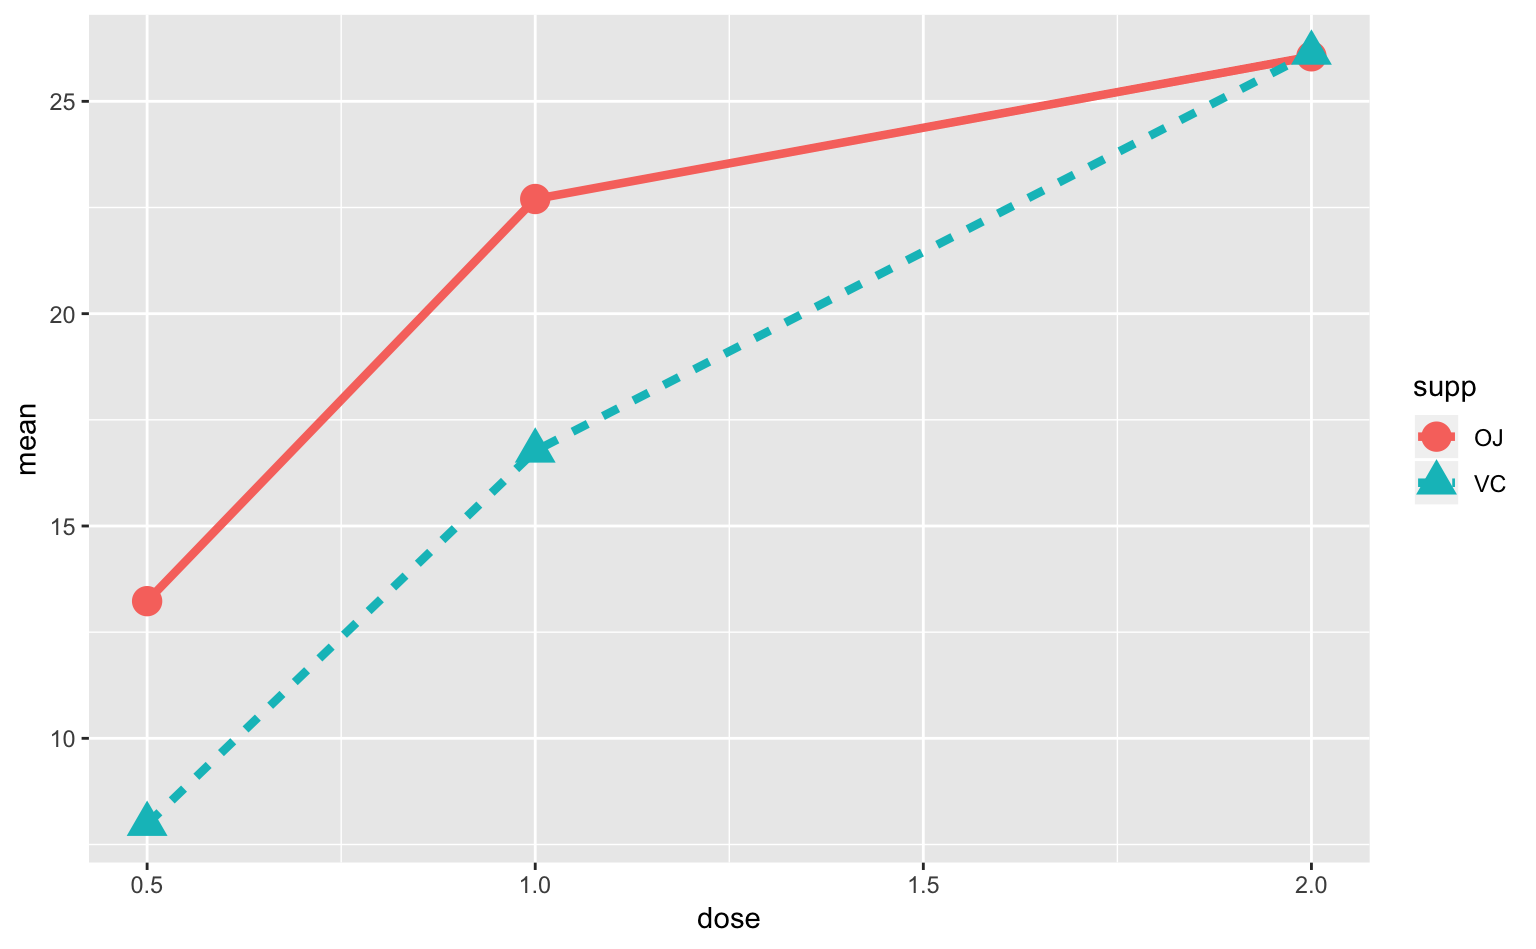
\includegraphics{lecture_note_files/figure-latex/unnamed-chunk-69-1} 

}

\caption{Figure
\ref{fig:line-graph-3}の折れ線の色と線種を\texttt{supp}ごとに変え、さらにドットを付け足したグラフ。}\label{fig:unnamed-chunk-69}
\end{figure}

\section{面グラフ}

時間に伴う数量の変化の大きさをグループごとに比較・強調したい際には、\textbf{面グラフ}(area
graph; area chart)が向いている。

ここでは、gcookbookの\texttt{uspopage}(1900〜2002年のアメリカの人口統計)を使ってみよう。

\begin{Shaded}
\begin{Highlighting}[]
\KeywordTok{head}\NormalTok{(uspopage)}
\end{Highlighting}
\end{Shaded}

\begin{verbatim}
##   Year AgeGroup Thousands
## 1 1900       <5      9181
## 2 1900     5-14     16966
## 3 1900    15-24     14951
## 4 1900    25-34     12161
## 5 1900    35-44      9273
## 6 1900    45-54      6437
\end{verbatim}

変数はそれぞれ、

\begin{itemize}
\item
  \texttt{Year}:年
\item
  \texttt{AgeGroup}:年齢のカテゴリ
\item
  \texttt{Thousands}:人口
\end{itemize}

を表している。面グラフは\texttt{geom\_area()}で描くことができる。また、グループごとに色分けするには、\texttt{fill}に変数を指定すれば良い。



\begin{Shaded}
\begin{Highlighting}[]
\KeywordTok{ggplot}\NormalTok{(uspopage, }\KeywordTok{aes}\NormalTok{(Year, Thousands, }\DataTypeTok{fill =}\NormalTok{ AgeGroup)) }\OperatorTok{+}\StringTok{ }\CommentTok{# x軸にYear、y軸にThousands;fill = AgeGroupと指定することで、自動で塗りつぶされる}
\StringTok{  }\KeywordTok{geom_area}\NormalTok{() }\CommentTok{# 面グラフ}
\end{Highlighting}
\end{Shaded}

\begin{figure}

{\centering 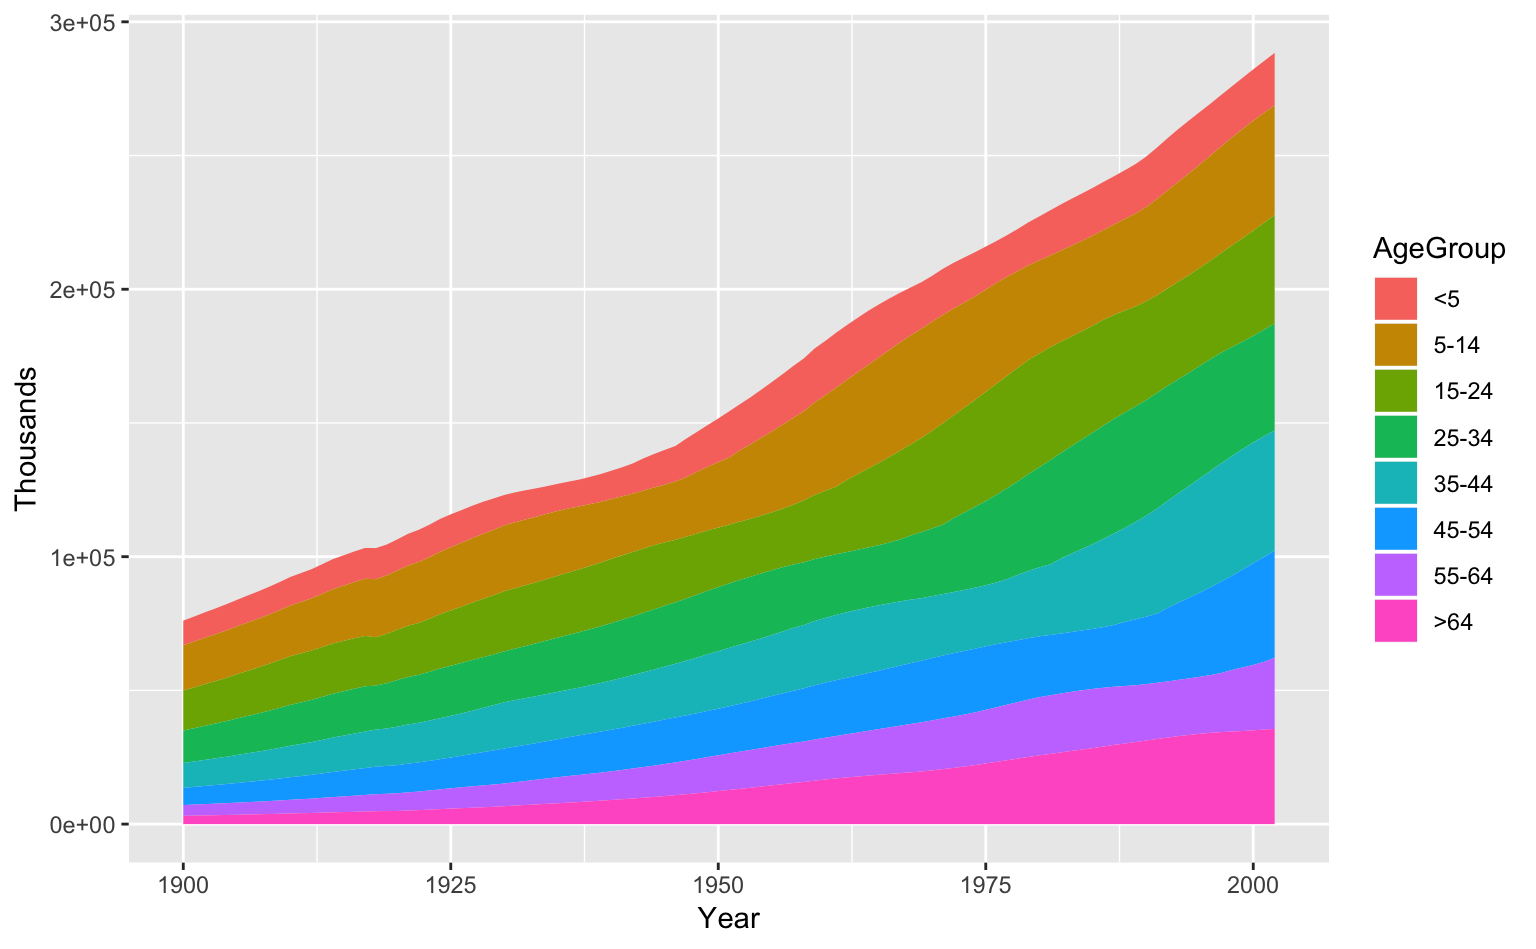
\includegraphics{lecture_note_files/figure-latex/unnamed-chunk-71-1} 

}

\caption{アメリカの人口の推移を表した面グラフ。}\label{fig:unnamed-chunk-71}
\end{figure}

\section{練習問題}\label{-3}

\begin{itemize}
\item
  ggplot2の\texttt{economics}データを使って、失業者数の推移をプロットしてみよう。
\item
  gcookbookの\texttt{worldpop}データをもとに、\texttt{geom\_line()}と\texttt{geom\_point()}を使い、世界人口の推移をプロットしてみよう。また、世界人口の素値ではなく常用対数をプロットするとどのようになるだろうか?(ヒント:\texttt{log10(変数)}で常用対数を計算することができる)
\end{itemize}

\chapter{推測統計}\label{statistics}

データの可視化では、推測統計量のプロットを含めることがしばしばである。

\begin{Shaded}
\begin{Highlighting}[]
\KeywordTok{library}\NormalTok{(ggplot2) }\CommentTok{# 忘れずにパッケージを読み込む}
\end{Highlighting}
\end{Shaded}

\section{エラーバー}

\textbf{エラーバー}(error
bar)は誰でも馴染みがあるのではないだろうか。棒グラフとよく一緒にいるアイツのことである。エラーバーはデータの\textbf{標準誤差}(standard
error of the mean; \emph{SEM}\footnote{構造方程式モデリング(structural
  equation modeling; SEM)のことではない。})を表すのに使われることが多い。

ここでは、gcookbookの\texttt{cabbage\_exp}(キャベツに関するデータセット)を使ってエラーバーを描いてみよう。

\begin{Shaded}
\begin{Highlighting}[]
\KeywordTok{library}\NormalTok{(gcookbook) }\CommentTok{# パッケージの読み込み}
\end{Highlighting}
\end{Shaded}

\begin{Shaded}
\begin{Highlighting}[]
\KeywordTok{head}\NormalTok{(cabbage_exp) }\CommentTok{#6行のデータなのですべて表示される}
\end{Highlighting}
\end{Shaded}

\begin{verbatim}
##   Cultivar Date Weight        sd  n         se
## 1      c39  d16   3.18 0.9566144 10 0.30250803
## 2      c39  d20   2.80 0.2788867 10 0.08819171
## 3      c39  d21   2.74 0.9834181 10 0.31098410
## 4      c52  d16   2.26 0.4452215 10 0.14079141
## 5      c52  d20   3.11 0.7908505 10 0.25008887
## 6      c52  d21   1.47 0.2110819 10 0.06674995
\end{verbatim}

注目する変数は、

\begin{itemize}
\item
  \texttt{Cultivar}:キャベツの品種(c39 or c52)
\item
  \texttt{Date}:栽培期間
\item
  \texttt{Weight}:キャベツの平均重量
\item
  \texttt{se}:キャベツの平均重量の標準誤差
\end{itemize}

である。平均値を棒グラフで、標準誤差をエラーバーで描いてみよう。コードは以下の通りである。

(ref:errorbar-1)
エラーバー付きの棒グラフ。エラーバーは標準誤差を表している。

\begin{Shaded}
\begin{Highlighting}[]
\KeywordTok{ggplot}\NormalTok{(cabbage_exp, }\KeywordTok{aes}\NormalTok{(Date, Weight, }\DataTypeTok{fill =}\NormalTok{ Cultivar)) }\OperatorTok{+}\StringTok{ }\CommentTok{# x軸にDate、y軸にWeight、Cultivarごとに色分け}
\StringTok{  }\KeywordTok{geom_bar}\NormalTok{(}\DataTypeTok{stat =} \StringTok{"identity"}\NormalTok{, }\DataTypeTok{position =} \StringTok{"dodge"}\NormalTok{) }\OperatorTok{+}\StringTok{ }\CommentTok{# グルーピングされた棒グラフの復習}
\StringTok{  }\KeywordTok{geom_errorbar}\NormalTok{(}\KeywordTok{aes}\NormalTok{(}\DataTypeTok{ymin =}\NormalTok{ Weight }\OperatorTok{-}\StringTok{ }\NormalTok{se, }\DataTypeTok{ymax =}\NormalTok{ Weight }\OperatorTok{+}\StringTok{ }\NormalTok{se), }\DataTypeTok{position =} \KeywordTok{position_dodge}\NormalTok{(}\DataTypeTok{width =} \FloatTok{0.9}\NormalTok{), }\DataTypeTok{width =} \FloatTok{0.2}\NormalTok{) }\CommentTok{# ymin:エラーバーの下端、ymax:エラーバーの上端}
\end{Highlighting}
\end{Shaded}

\begin{figure}

{\centering 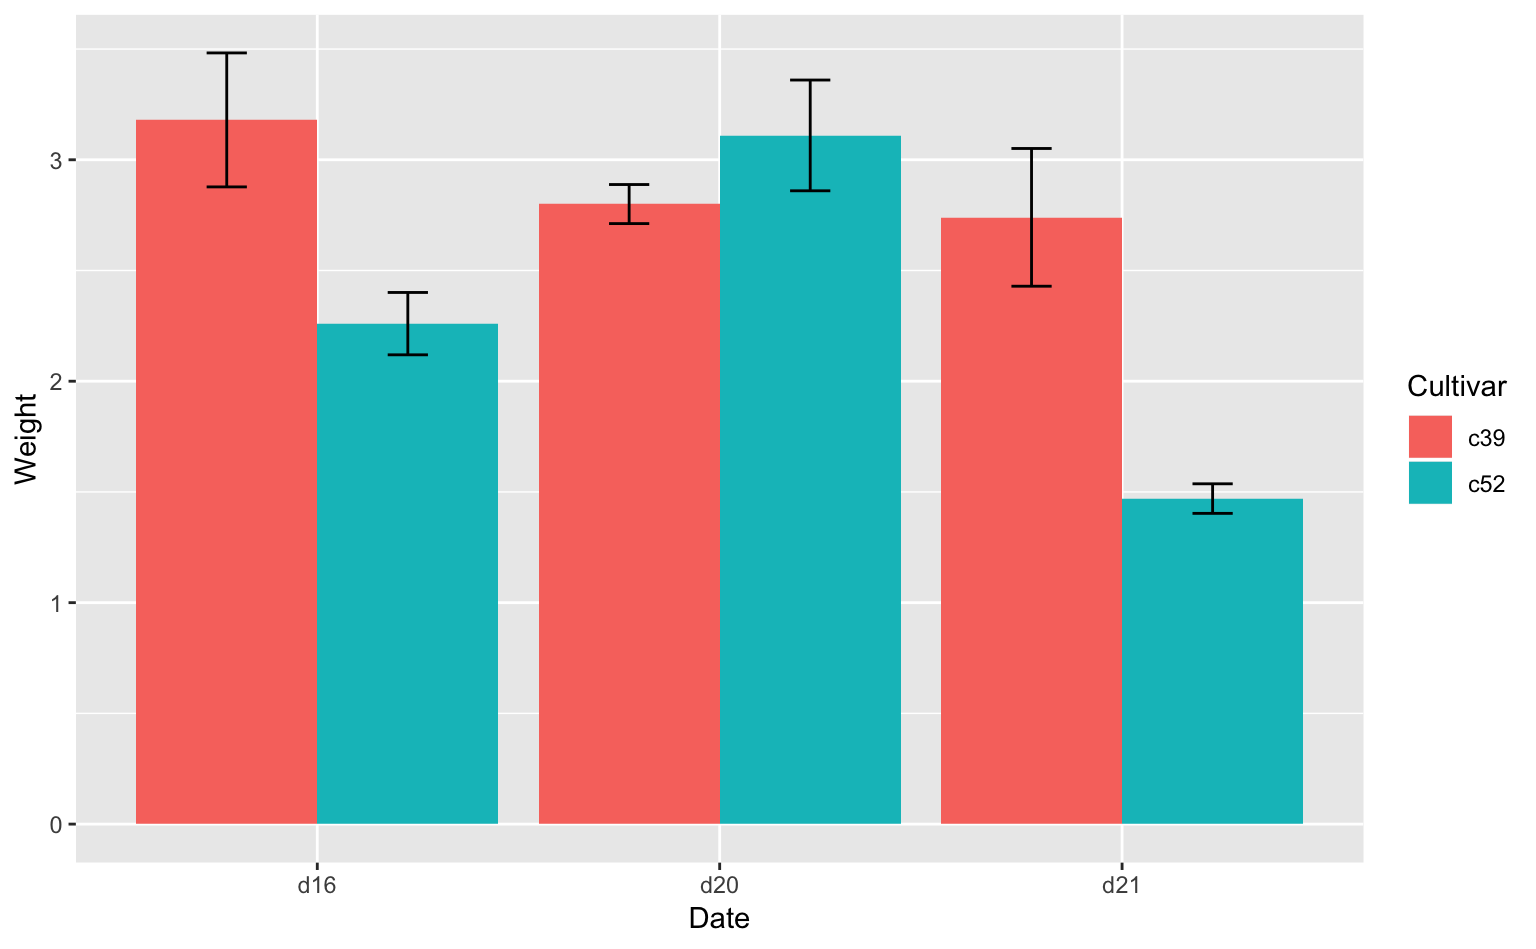
\includegraphics{lecture_note_files/figure-latex/errorbar-1-1} 

}

\caption{(ref:errorbar-1)}\label{fig:errorbar-1}
\end{figure}

コードの内容を順に解説する。

\begin{enumerate}
\def\labelenumi{\arabic{enumi}.}
\setcounter{enumi}{-1}
\item
  \texttt{ggplot(cabbage\_exp,\ aes(Date,\ Weight,\ fill\ =\ Cultivar)}

  \begin{itemize}
  \tightlist
  \item
    x軸に\texttt{Date}、y軸に\texttt{Weight}、グルーピング(塗りつぶし)に\texttt{Cultivar}を指定。
  \end{itemize}
\item
  \texttt{geom\_bar(stat\ =\ "identity",\ position\ =\ "dodge")}

  \begin{itemize}
  \item
    棒グラフ。\texttt{stat\ =\ "identity"}とする必要がある。また、\texttt{Cultivar}ごとに位置をずらすには、\texttt{position\ =\ "dodge"}としなければならない。
  \item
    忘れてしまった人は、もう一度Chapter \ref{amount}を復習しよう。
  \end{itemize}
\item
  \texttt{geom\_errorbar(aes(ymin\ =\ Weight\ -\ se,\ ymax\ =\ Weight\ +\ se),\ position\ =\ position\_dodge(width\ =\ 0.9),\ width\ =\ 0.2)}

  \begin{itemize}
  \item
    エラーバー。\texttt{ymin}と\texttt{ymax}には、それぞれエラーバーの下端と上端のy座標を指定する。
  \item
    \texttt{position\ =\ position\_dodge(width\ =\ 0.9)}とすることで、エラーバーを棒グラフのように水平方向にずらすことができる。棒グラフのずらし幅が0.9なので、エラーバーの\texttt{width}(ずらし幅)も0.9にする\footnote{ちなみに、今まで出てきた\texttt{position\ =\ "dodge"}は\texttt{position\ =\ position\_dodge()}の省略版である。}。
  \item
    最後の\texttt{width}はエラーバーの横幅を表している。デフォルトだと、棒グラフの棒と同じ幅になる。
  \end{itemize}
\end{enumerate}

なお、\textbf{エラーバーを描く際は、エラーバーが何を表しているのかをキャプションなどに含めなければならない。}なぜなら、エラーバーは標準誤差、95\%信頼区間(95\%
confidence interval; 95\%
CI)、標準偏差、ベイズ信頼区間など、様々な統計量を表現するのにも使われるからである。

\section{信頼区間}

信頼区間のプロットにも\texttt{geom\_errorbar()}は使えるが、折れ線グラフ(時系列データ)などでは\texttt{geom\_ribbon()}の方が良いだろう。ここでは、gcookbookの\texttt{climate}(気温の時系列データ)を使ってみよう。

\begin{Shaded}
\begin{Highlighting}[]
\KeywordTok{head}\NormalTok{(climate)}
\end{Highlighting}
\end{Shaded}

\begin{verbatim}
##     Source Year Anomaly1y Anomaly5y Anomaly10y Unc10y
## 1 Berkeley 1800        NA        NA     -0.435  0.505
## 2 Berkeley 1801        NA        NA     -0.453  0.493
## 3 Berkeley 1802        NA        NA     -0.460  0.486
## 4 Berkeley 1803        NA        NA     -0.493  0.489
## 5 Berkeley 1804        NA        NA     -0.536  0.483
## 6 Berkeley 1805        NA        NA     -0.541  0.475
\end{verbatim}

なお、ここでは\texttt{Source}が\texttt{"Berkeley"}のデータだけを抽出して可視化を行う。抽出したデータは\texttt{clim}に代入する。以下のコードは今は理解できなくて良い。

\begin{Shaded}
\begin{Highlighting}[]
\KeywordTok{library}\NormalTok{(tidyverse) }\CommentTok{# データハンドリング用のパッケージ群を読み込む}
\end{Highlighting}
\end{Shaded}

\begin{Shaded}
\begin{Highlighting}[]
\NormalTok{clim =}\StringTok{ }\NormalTok{climate }\OperatorTok\StringTok{ }\CommentTok{# climateデータの}
\StringTok{  }\KeywordTok{filter}\NormalTok{(Source }\OperatorTok{==}\StringTok{ "Berkeley"}\NormalTok{) }\CommentTok{# Sourceが"Berkeley"の行だけを抽出してください}
\end{Highlighting}
\end{Shaded}

プロットするのは以下の変数である。

\begin{itemize}
\item
  \texttt{Year}:年
\item
  \texttt{Anomaly10y}:1951〜1980年の平均気温と比べたときのズレ
\item
  \texttt{Unc10y}:95\%信頼区間
\end{itemize}

では、\texttt{geom\_ribbon()}を使ってプロットしてみよう。コードの書き方は\texttt{geom\_errorbar()}に似ている。なお、\texttt{alpha}で信頼区間を半透明にしないと、グラフが真っ黒になってしまうので注意が必要である。



\begin{Shaded}
\begin{Highlighting}[]
\KeywordTok{ggplot}\NormalTok{(clim, }\KeywordTok{aes}\NormalTok{(Year, Anomaly10y)) }\OperatorTok{+}
\StringTok{  }\KeywordTok{geom_line}\NormalTok{() }\OperatorTok{+}
\StringTok{  }\KeywordTok{geom_ribbon}\NormalTok{(}\KeywordTok{aes}\NormalTok{(}\DataTypeTok{ymin =}\NormalTok{ Anomaly10y }\OperatorTok{-}\StringTok{ }\NormalTok{Unc10y, }\DataTypeTok{ymax =}\NormalTok{ Anomaly10y }\OperatorTok{+}\StringTok{ }\NormalTok{Unc10y), }\DataTypeTok{alpha =} \FloatTok{0.2}\NormalTok{) }\CommentTok{# alphaで透明度を指定}
\end{Highlighting}
\end{Shaded}

\begin{figure}

{\centering 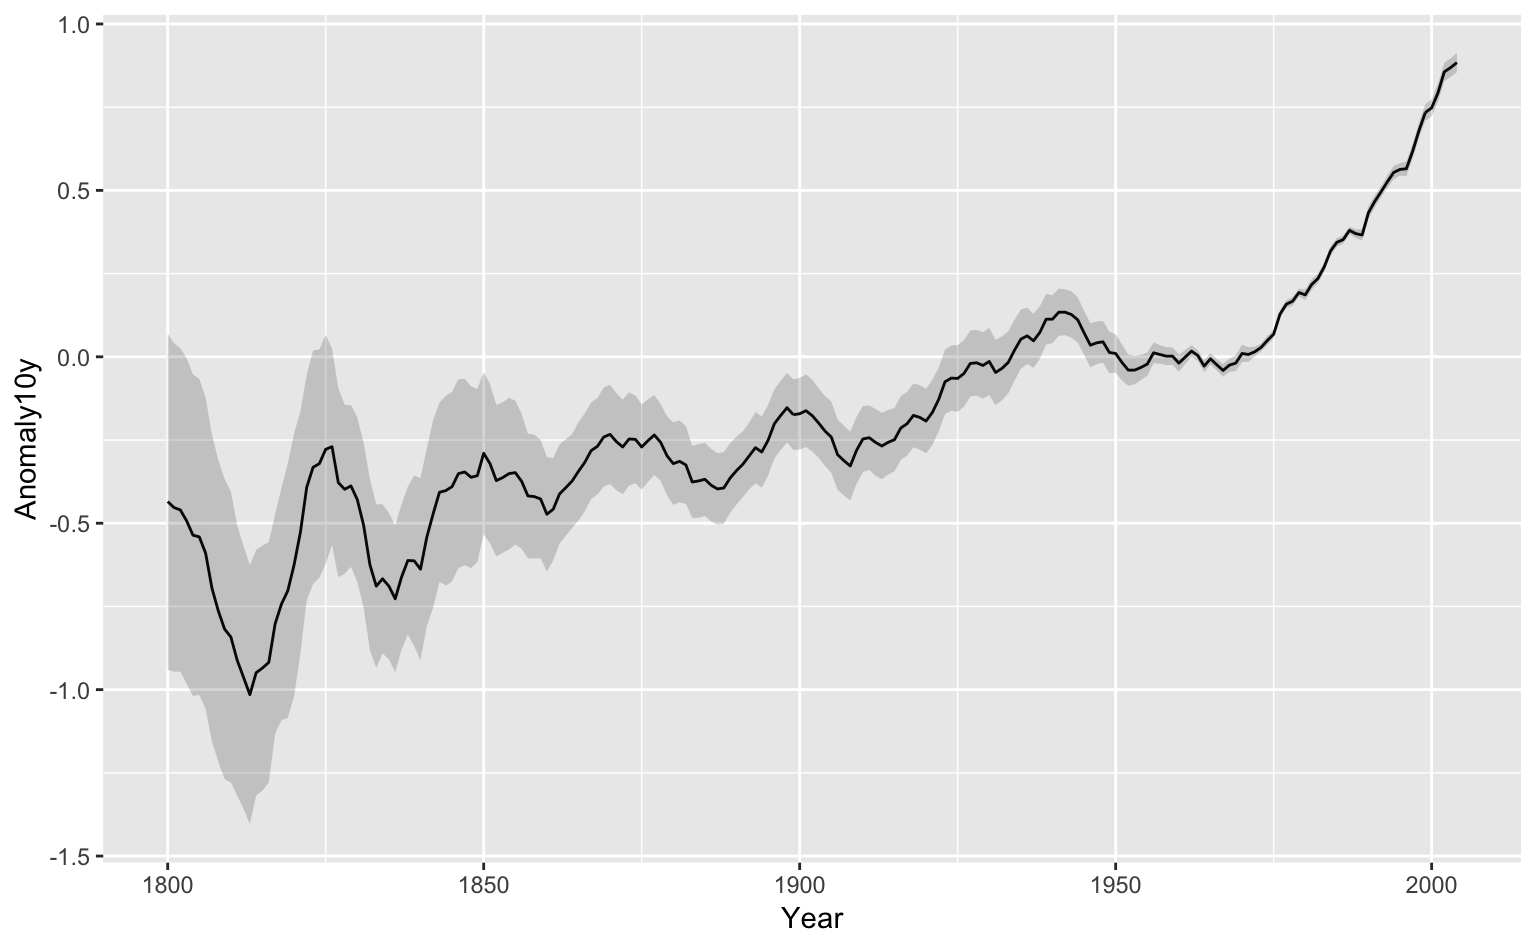
\includegraphics{lecture_note_files/figure-latex/unnamed-chunk-82-1} 

}

\caption{95\%信頼区間のプロット。}\label{fig:unnamed-chunk-82}
\end{figure}

\section{回帰直線などのフィッティング}

散布図に回帰直線などをフィッティングさせた図を見たことがあるだろう。ggplot2でもそれが可能である。ここでは、gcookbookの\texttt{heightweight}(こどもの身長と体重データ)を使ってみよう。

\begin{Shaded}
\begin{Highlighting}[]
\KeywordTok{head}\NormalTok{(heightweight) }\CommentTok{# 先頭6行}
\end{Highlighting}
\end{Shaded}

\begin{verbatim}
##   sex ageYear ageMonth heightIn weightLb
## 1   f   11.92      143     56.3     85.0
## 2   f   12.92      155     62.3    105.0
## 3   f   12.75      153     63.3    108.0
## 4   f   13.42      161     59.0     92.0
## 5   f   15.92      191     62.5    112.5
## 6   f   14.25      171     62.5    112.0
\end{verbatim}

まず、\texttt{geom\_point()}で身長(\texttt{heightIn})と体重(\texttt{WeightLb})の散布図を描き、その上に\texttt{geom\_smooth()}で回帰直線を描いてみよう。なお、回帰直線を引くには、\texttt{method\ =\ lm}と指定する必要がある(デフォルトだとLOESS曲線\footnote{\url{https://en.wikipedia.org/wiki/Local_regression}}
が引かれる)。Rにおいて\texttt{lm}は線形モデル(linear
model)を表している。

(ref:smooth-plot-1)
散布図の上に回帰直線を描いたグラフ。網掛けの部分は95\%信頼区間を表している。

\begin{Shaded}
\begin{Highlighting}[]
\KeywordTok{ggplot}\NormalTok{(heightweight, }\KeywordTok{aes}\NormalTok{(ageYear, heightIn)) }\OperatorTok{+}
\StringTok{  }\KeywordTok{geom_point}\NormalTok{() }\OperatorTok{+}\StringTok{ }\CommentTok{# まず散布図}
\StringTok{  }\KeywordTok{geom_smooth}\NormalTok{(}\DataTypeTok{method =}\NormalTok{ lm) }\CommentTok{# それから回帰直線;method = lmと指定する必要あり}
\end{Highlighting}
\end{Shaded}

\begin{figure}

{\centering 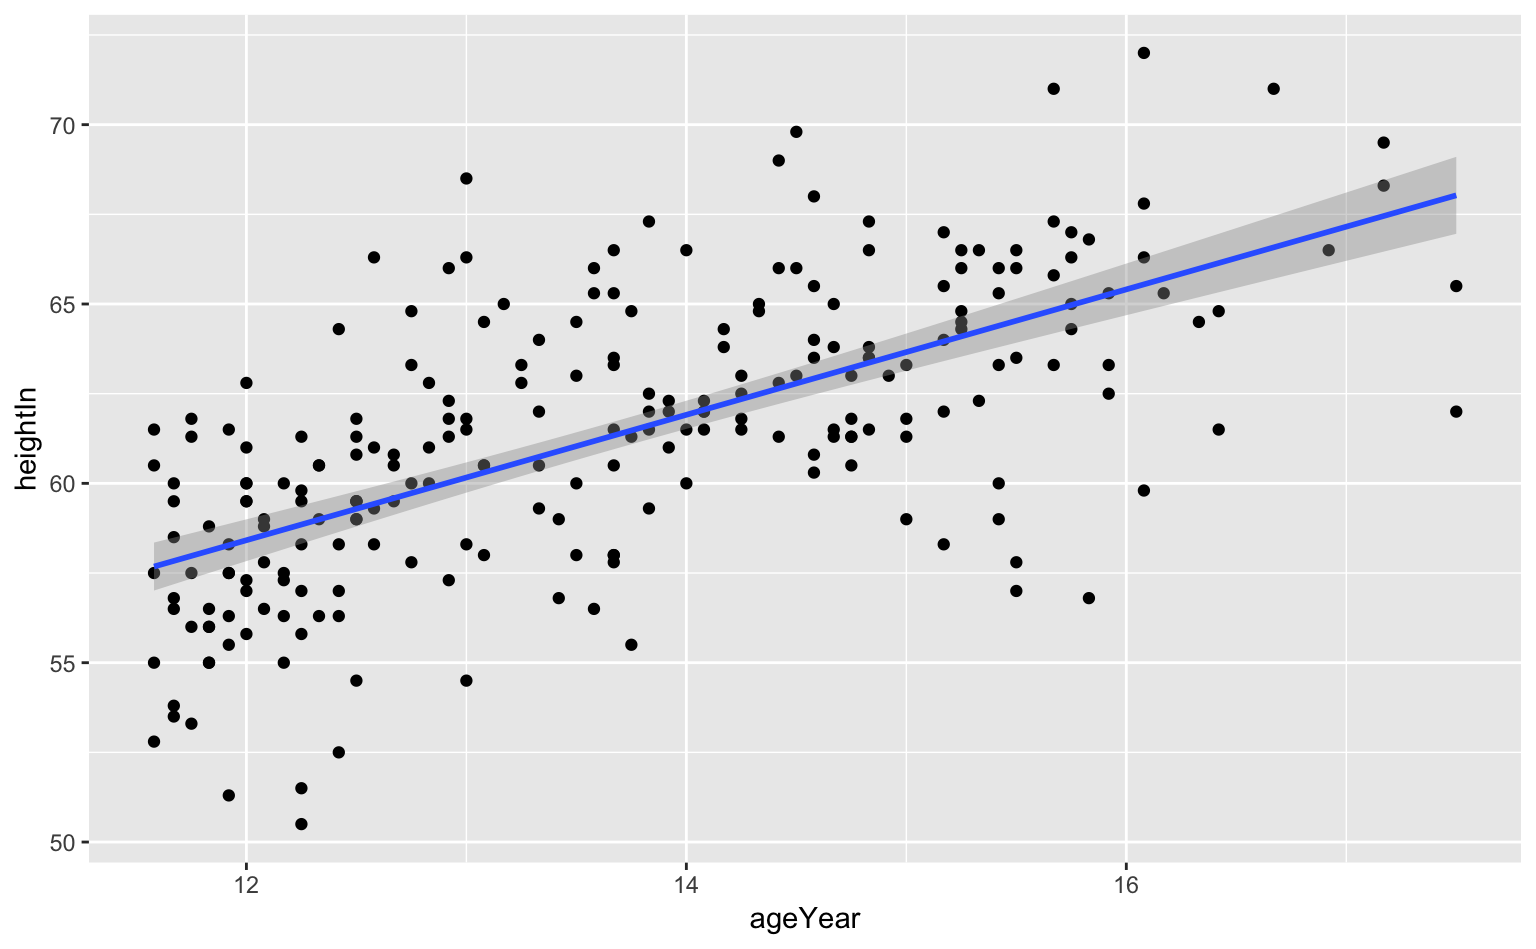
\includegraphics{lecture_note_files/figure-latex/unnamed-chunk-84-1} 

}

\caption{(ref:smooth-plot-1)}\label{fig:unnamed-chunk-84}
\end{figure}

グループごとに回帰直線を引きたい場合は、\texttt{fill}にグルーピングの変数を指定すれば良い。

(ref:smooth-plot-2)
こどもの性別ごとに回帰直線を描いたグラフ。網掛けの部分は95\%信頼区間を表している。

\begin{Shaded}
\begin{Highlighting}[]
\KeywordTok{ggplot}\NormalTok{(heightweight, }\KeywordTok{aes}\NormalTok{(ageYear, heightIn, }\DataTypeTok{fill =}\NormalTok{ sex)) }\OperatorTok{+}\StringTok{ }\CommentTok{# fill = sexを追加}
\StringTok{  }\KeywordTok{geom_point}\NormalTok{() }\OperatorTok{+}
\StringTok{  }\KeywordTok{geom_smooth}\NormalTok{(}\DataTypeTok{method =}\NormalTok{ lm)}
\end{Highlighting}
\end{Shaded}

\begin{figure}

{\centering 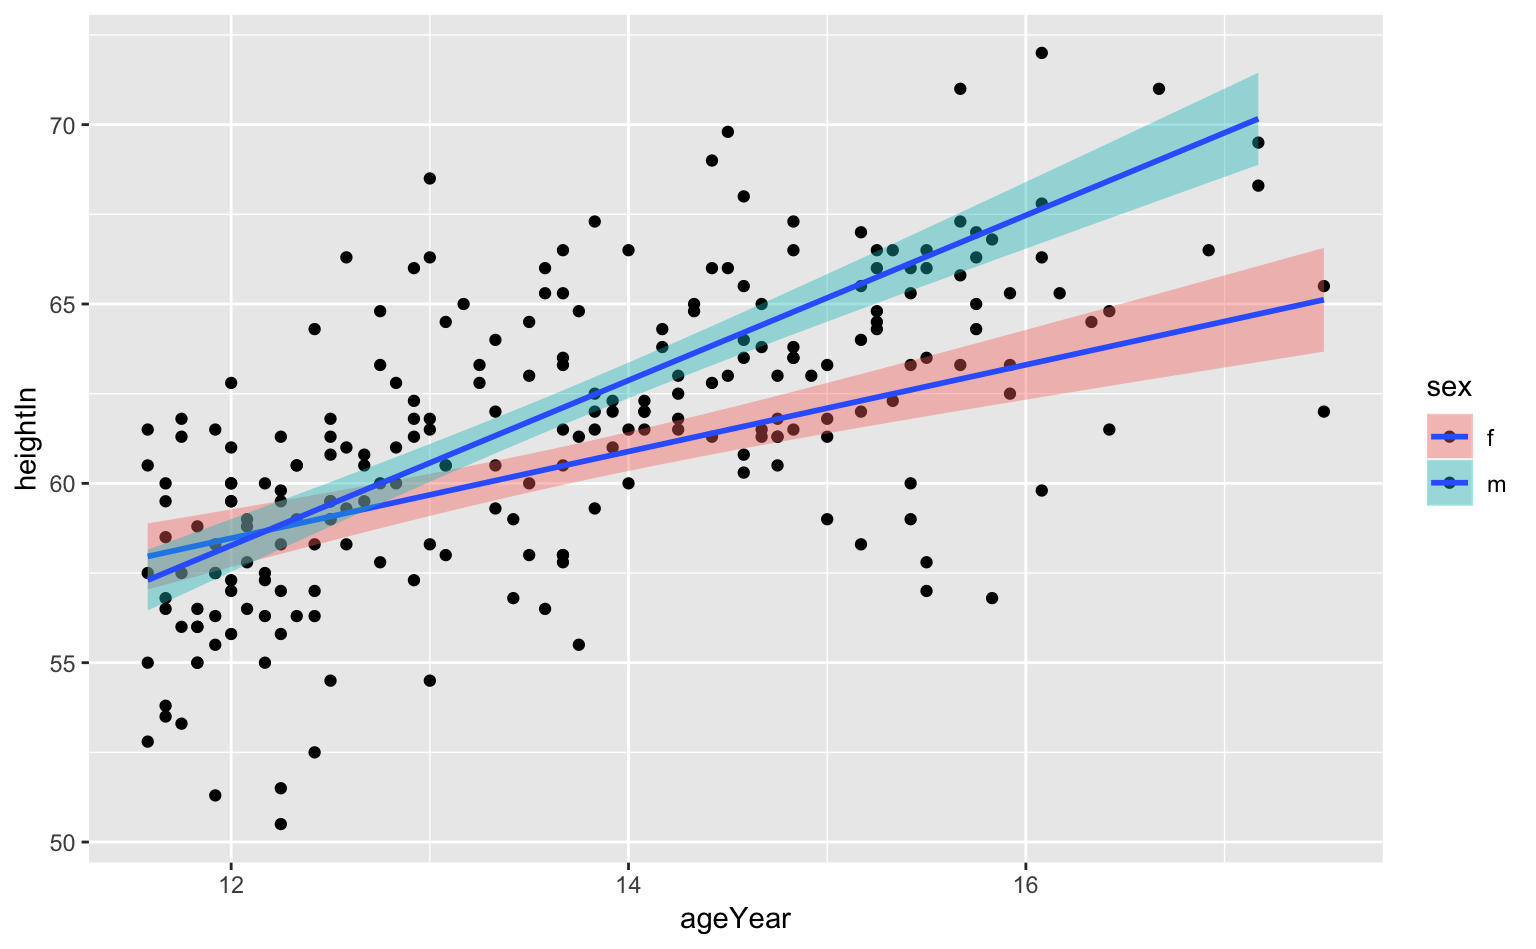
\includegraphics{lecture_note_files/figure-latex/unnamed-chunk-85-1} 

}

\caption{(ref:smooth-plot-2)}\label{fig:unnamed-chunk-85}
\end{figure}

もちろん、線形モデル以外のフィッティングも可能である。詳しくはGoogle先生が教えてくれるだろう。

\section{練習問題}\label{-4}

\begin{itemize}
\item
  Figure
  \ref{fig:errorbar-1}で描いた\texttt{cabbage\_exp}データの平均値と標準誤差を、今度は折れ線グラフとエラーバーで描いてみよう。このとき、エラーバーはどれくらい調整すれば良いだろうか?
\item
  Rにデフォルトで入っている\texttt{faithful}データの散布図を描き、その上に回帰直線をプロットしてみよう。
\end{itemize}

\chapter{図の体裁}\label{appearance}

ggplot2はデフォルトでも十分見栄えの良いグラフを出力してくれる。しかし、より見やすいグラフを作るために少し工夫しなければならない場面もある。また、最後にグラフの保存方法などを解説する。

\begin{Shaded}
\begin{Highlighting}[]
\KeywordTok{library}\NormalTok{(ggplot2) }\CommentTok{# 忘れずにパッケージを読み込む}
\end{Highlighting}
\end{Shaded}

\section{軸の反転}

人間誰しも、グラフの軸を反転させたくなるときがある\footnote{異論は\ldots{}\ldots{}。}。Figure
\ref{fig:dot-plot}
のClevelandのドットプロットのように\texttt{x}と\texttt{y}の変数を逆にしても良いが、ggplot2の設計上それではうまくいかない場合もある。

そのようなときは\texttt{coord\_flip()}を使えば良い。これは文字通り、座標(coordination)と反転(flip)させるための関数である。

たとえば、Figure
\ref{fig:bar-plot-3}で\texttt{diamonds}データ(\texttt{cut}ごとのダイアモンドの個数)をプロットしたが、これに\texttt{coord\_flip()}を付け足すと以下のようになる。



\begin{Shaded}
\begin{Highlighting}[]
\KeywordTok{ggplot}\NormalTok{(diamonds, }\KeywordTok{aes}\NormalTok{(cut)) }\OperatorTok{+}\StringTok{ }\CommentTok{# x軸にcut;yには何も対応づける必要なし}
\StringTok{  }\KeywordTok{geom_bar}\NormalTok{() }\OperatorTok{+}\StringTok{ }\CommentTok{# 棒グラフ;データの値ではなく個数を描くので、stat = "identity"は不要}
\StringTok{  }\KeywordTok{coord_flip}\NormalTok{() }\CommentTok{# 軸を反転}
\end{Highlighting}
\end{Shaded}

\begin{figure}

{\centering 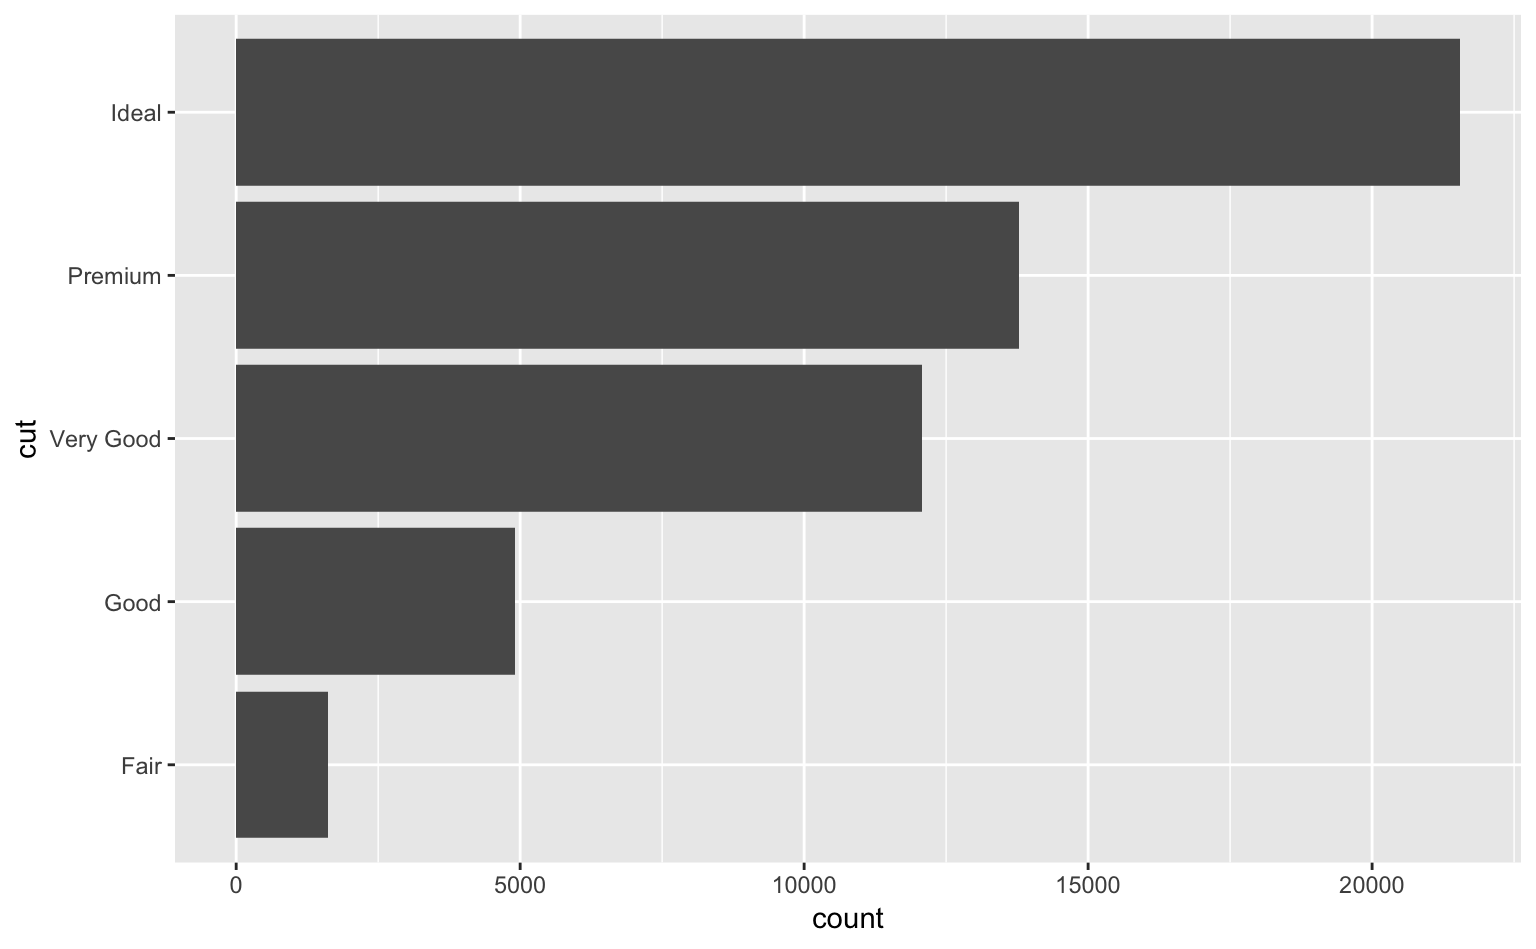
\includegraphics{lecture_note_files/figure-latex/unnamed-chunk-90-1} 

}

\caption{Figure \ref{fig:bar-plot-3}の軸を反転させたグラフ。}\label{fig:unnamed-chunk-90}
\end{figure}

\section{Small multiple}\label{small-multiple}

プロットする変数が多く、1枚にまとめると見づらくなってしまう場合、グラフを複数個の小さなパネル(サブプロット)に分割して並べると見やすくなる。これをSmall
multiple\footnote{\url{https://en.wikipedia.org/wiki/Small_multiple}}という
。Small
multipleは\texttt{facet\_grid()}もしくは\texttt{facet\_wrap()}で作ることができる。

たとえば、Chapter \ref{association}で作った\texttt{mpg}の散布図(Figure
\ref{fig:scatter-plot-4})は、\texttt{drv}と\texttt{cyl}という変数によって、以下のような小さなパネルに分割することができる。描き方は、\texttt{facet\_grid(行方向の変数\textasciitilde{}列方向の変数)}である。

(ref:facet-1)
\texttt{facet\_grid()}を使った例。パネルが行列の形で表示される。

\begin{Shaded}
\begin{Highlighting}[]
\KeywordTok{ggplot}\NormalTok{(mpg, }\KeywordTok{aes}\NormalTok{(displ, hwy)) }\OperatorTok{+}
\StringTok{  }\KeywordTok{geom_point}\NormalTok{() }\OperatorTok{+}
\StringTok{  }\KeywordTok{facet_grid}\NormalTok{(drv }\OperatorTok{~}\StringTok{ }\NormalTok{cyl) }\CommentTok{# drvは行方向、cylは列方向}
\end{Highlighting}
\end{Shaded}

\begin{figure}

{\centering 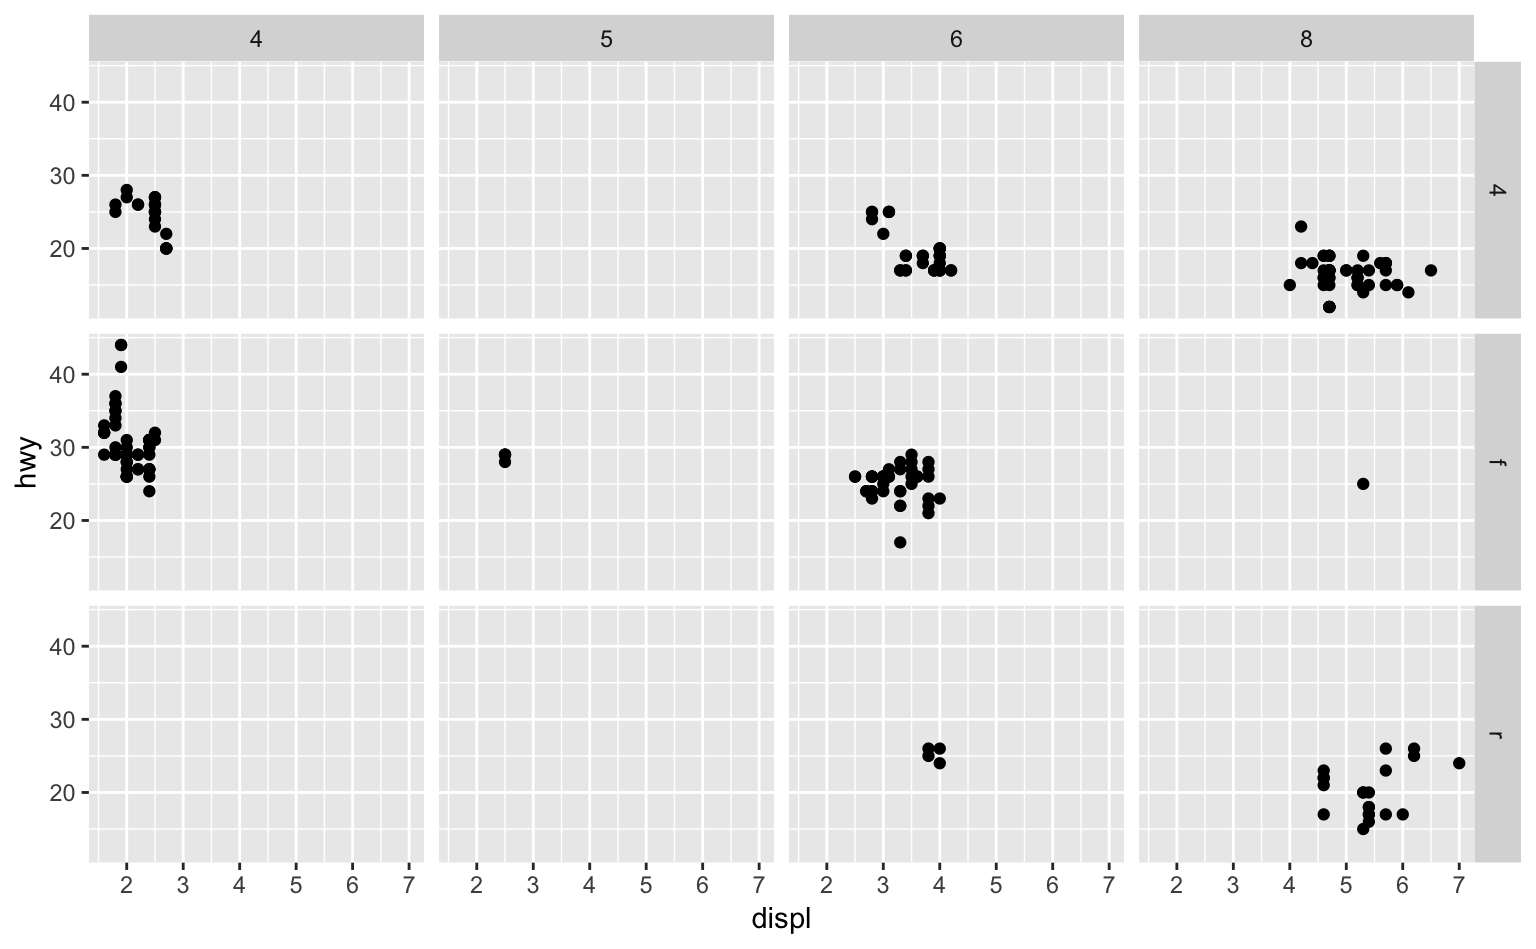
\includegraphics{lecture_note_files/figure-latex/facet-1-1} 

}

\caption{(ref:facet-1)}\label{fig:facet-1}
\end{figure}

\begin{center}\rule{0.5\linewidth}{\linethickness}\end{center}

一方、\texttt{facet\_wrap()}を使うと、2変数(\texttt{drv}と\texttt{cyl})が入れ子構造でプロットされるようになる。デフォルトでは縦横の枚数が同じになるが、\texttt{nrow}および\texttt{ncol}で行と列の数を指定できる。




\begin{Shaded}
\begin{Highlighting}[]
\KeywordTok{ggplot}\NormalTok{(mpg, }\KeywordTok{aes}\NormalTok{(displ, hwy)) }\OperatorTok{+}
\StringTok{  }\KeywordTok{geom_point}\NormalTok{() }\OperatorTok{+}
\StringTok{  }\KeywordTok{facet_wrap}\NormalTok{(drv }\OperatorTok{~}\StringTok{ }\NormalTok{cyl) }\CommentTok{# 入れ子構造でプロット}
\end{Highlighting}
\end{Shaded}

\begin{figure}

{\centering 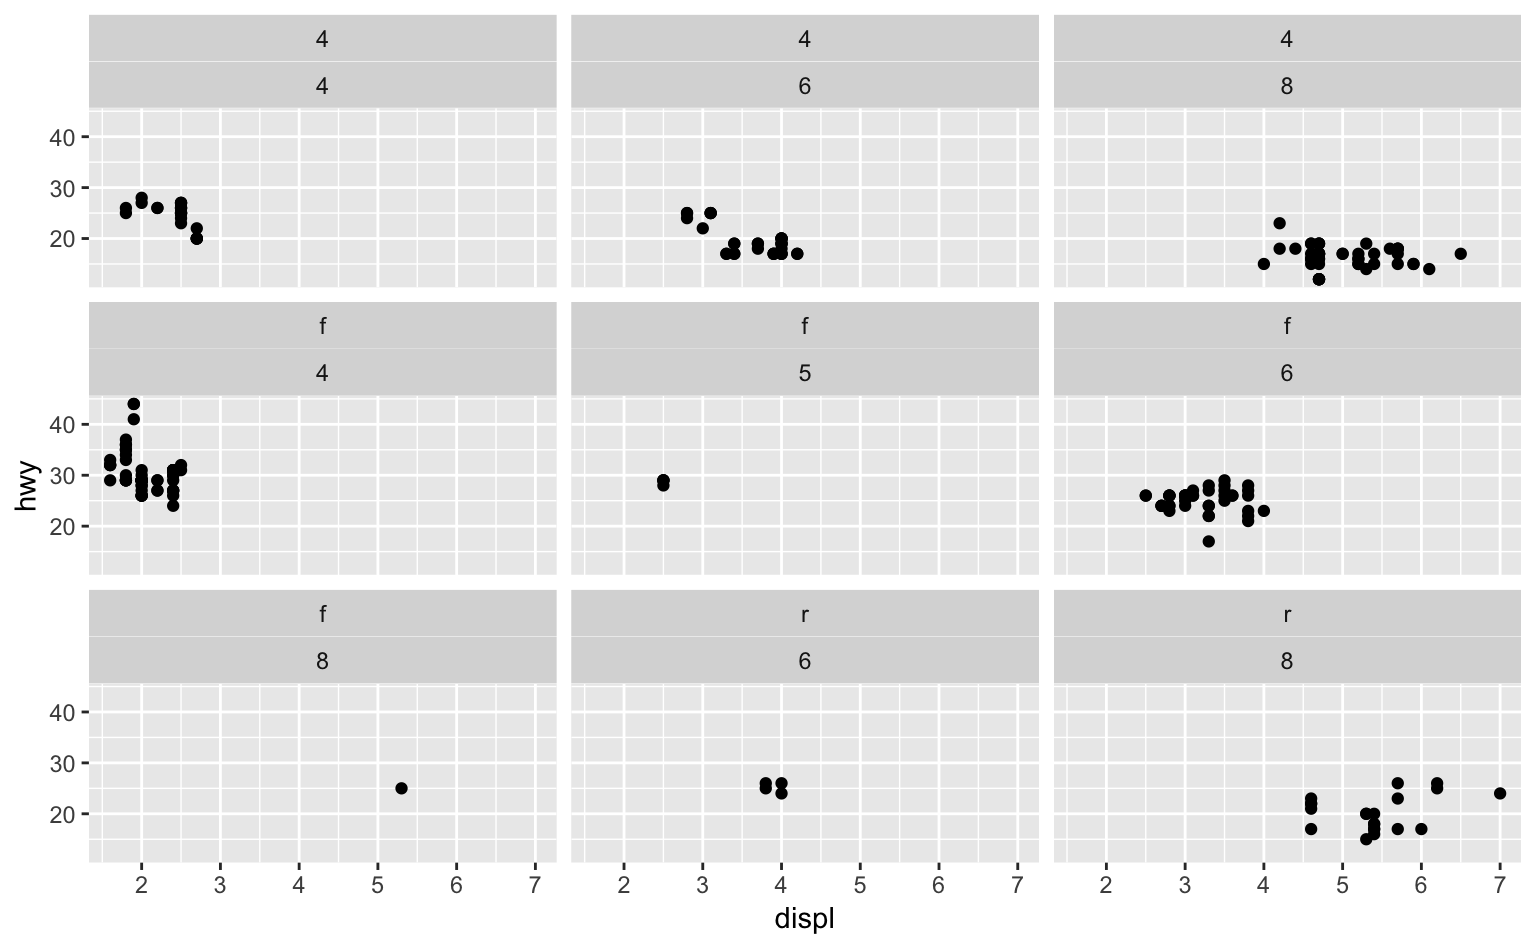
\includegraphics{lecture_note_files/figure-latex/unnamed-chunk-91-1} 

}

\caption{\texttt{facet\_wrap()}を使った例。上のFigure
\ref{fig:facet-1}と見比べてみよう。}\label{fig:unnamed-chunk-91}
\end{figure}

なお、\texttt{facet\_grid()}と\texttt{facet\_wrap()}の両方共、1変数だけでパネルを分けることも可能である。詳しくはヘルプ(\texttt{?facet\_grid()}または\texttt{?facet\_wrap()})で確認してほしい。

\section{テーマ}

グラフの全体的な体裁は、\texttt{theme\_xxxx()}で変えることができる。下の図の\texttt{theme\_gray()}はggplot2のデフォルトのテーマである。



\begin{Shaded}
\begin{Highlighting}[]
\KeywordTok{ggplot}\NormalTok{(mtcars, }\KeywordTok{aes}\NormalTok{(wt, mpg)) }\OperatorTok{+}
\StringTok{  }\KeywordTok{geom_point}\NormalTok{() }\OperatorTok{+}
\StringTok{  }\KeywordTok{theme_gray}\NormalTok{()}
\end{Highlighting}
\end{Shaded}

\begin{figure}

{\centering 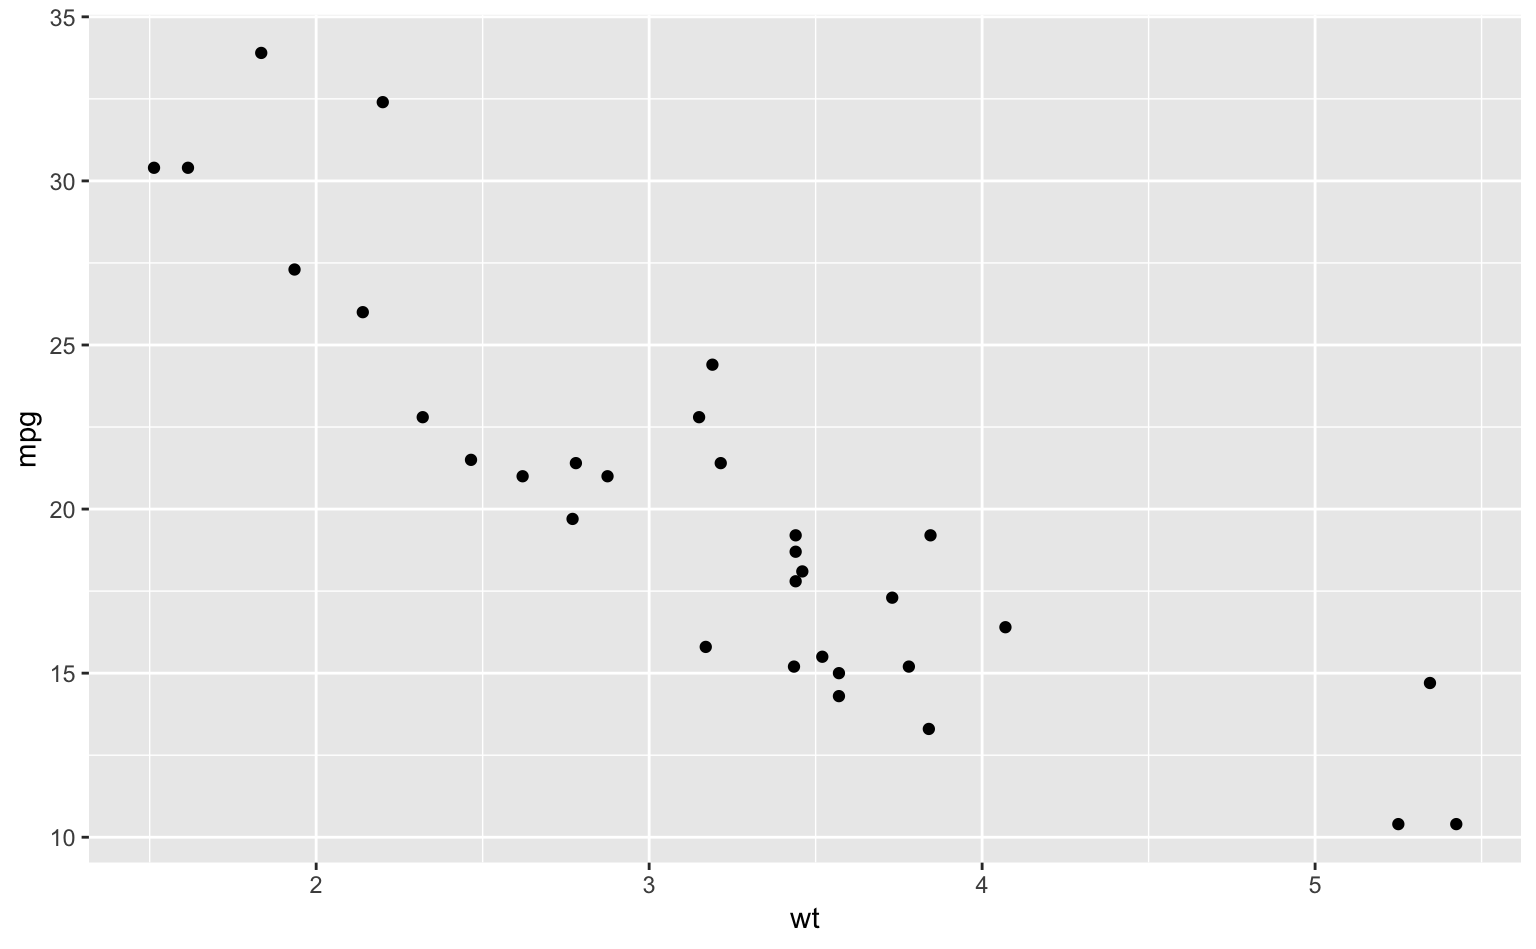
\includegraphics{lecture_note_files/figure-latex/unnamed-chunk-92-1} 

}

\caption{\texttt{theme\_gray()}を使った図(デフォルトのテーマ)。}\label{fig:unnamed-chunk-92}
\end{figure}

論文用の図として作ったり、大きなディスプレイに映したりする場合は、\texttt{theme\_bw()}または\texttt{theme\_classic()}が良いだろう。



\begin{Shaded}
\begin{Highlighting}[]
\KeywordTok{ggplot}\NormalTok{(mtcars, }\KeywordTok{aes}\NormalTok{(wt, mpg)) }\OperatorTok{+}
\StringTok{  }\KeywordTok{geom_point}\NormalTok{() }\OperatorTok{+}
\StringTok{  }\KeywordTok{theme_bw}\NormalTok{()}
\end{Highlighting}
\end{Shaded}

\begin{figure}

{\centering 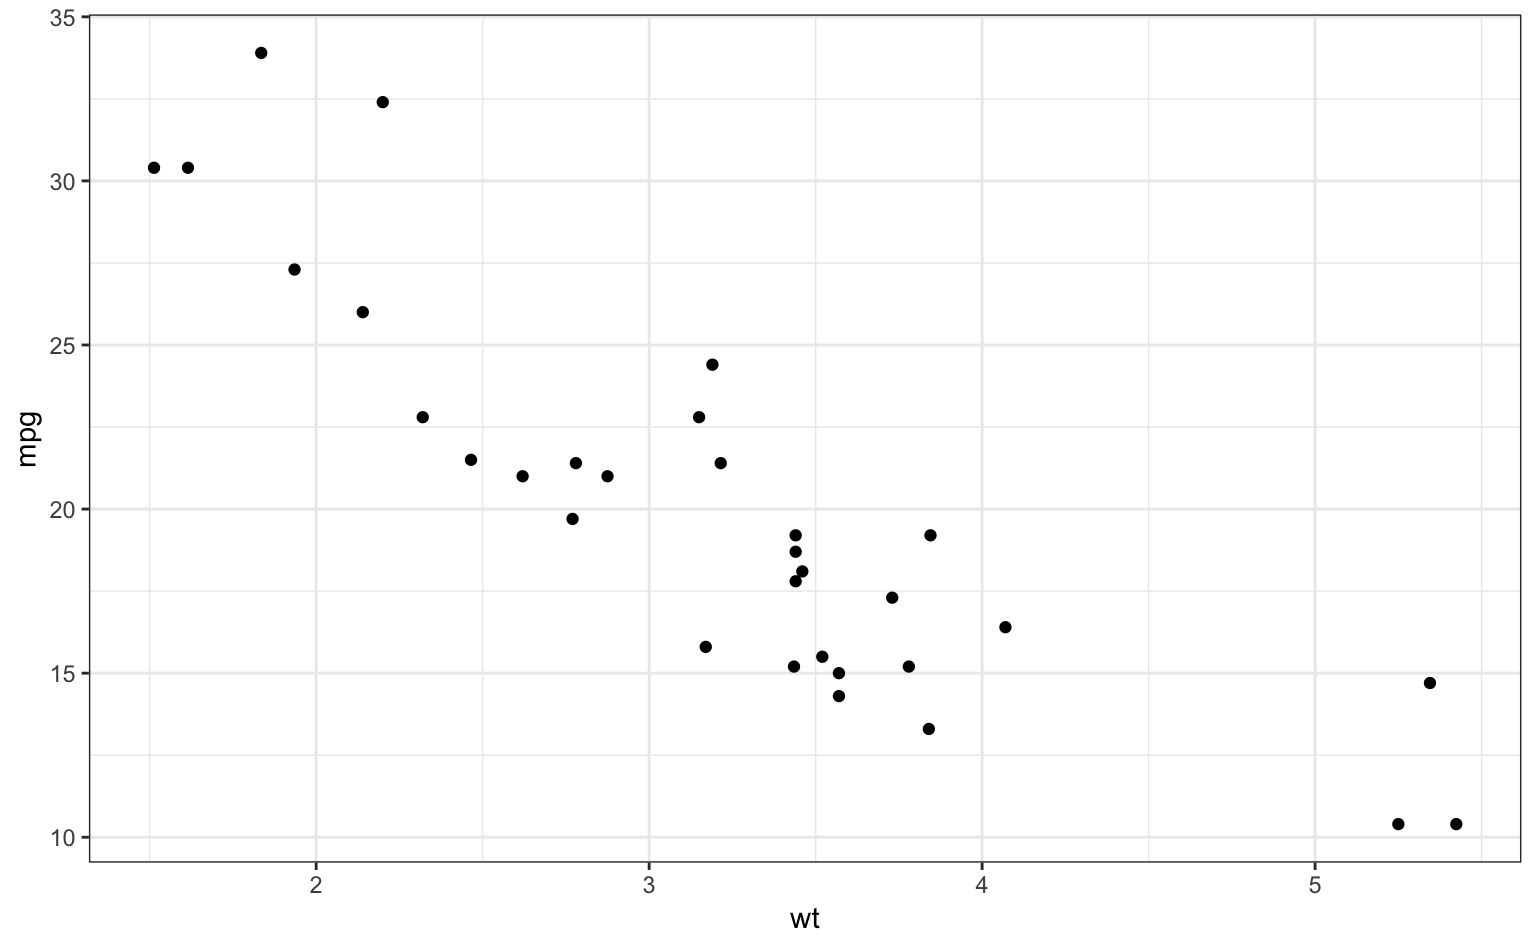
\includegraphics{lecture_note_files/figure-latex/unnamed-chunk-93-1} 

}

\caption{\texttt{theme\_bw()}を使った図。}\label{fig:unnamed-chunk-93}
\end{figure}



\begin{Shaded}
\begin{Highlighting}[]
\KeywordTok{ggplot}\NormalTok{(mtcars, }\KeywordTok{aes}\NormalTok{(wt, mpg)) }\OperatorTok{+}
\StringTok{  }\KeywordTok{geom_point}\NormalTok{() }\OperatorTok{+}
\StringTok{  }\KeywordTok{theme_classic}\NormalTok{()}
\end{Highlighting}
\end{Shaded}

\begin{figure}

{\centering 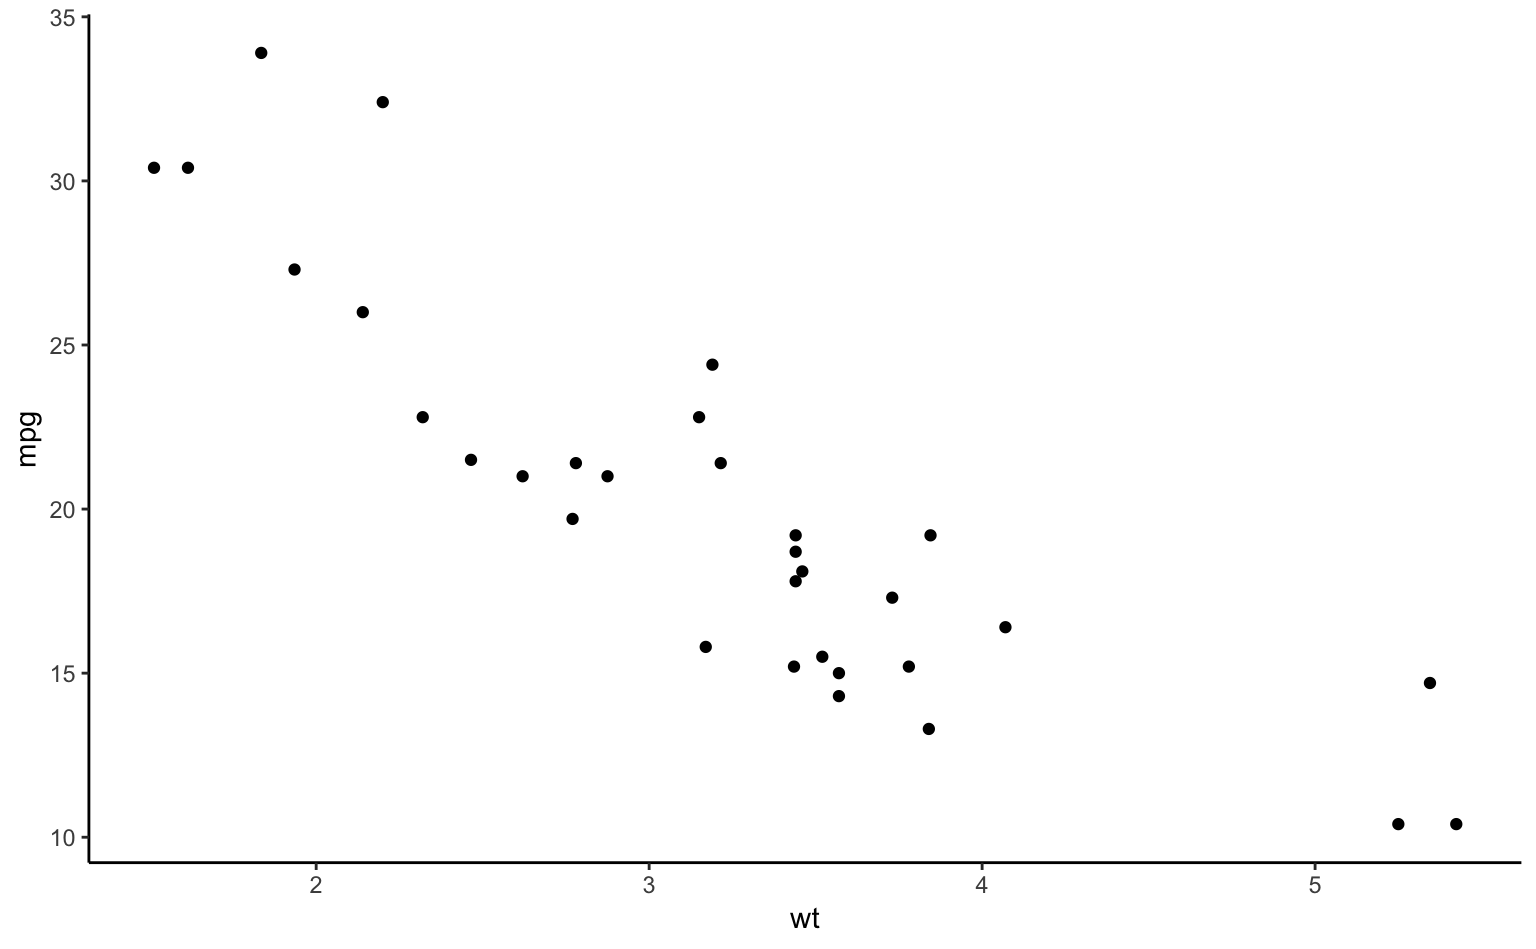
\includegraphics{lecture_note_files/figure-latex/unnamed-chunk-94-1} 

}

\caption{\texttt{theme\_classic()}を使った図。}\label{fig:unnamed-chunk-94}
\end{figure}

その他のテーマについては、\url{https://ggplot2.tidyverse.org/reference/ggtheme.html}
を見てほしい。

\section{色}

今までのグラフで散々見てきたように、\texttt{fill}や\texttt{color}でグルーピングを行うと、ggplot2のデフォルトのパステルカラーが適用される。ただ、この色は変えたい場合が多いだろう。

たとえば、下のように\texttt{scale\_color\_manual()}という関数を使うと、\texttt{color}で指定した変数を自分の好きな色に変えることができる\footnote{なお、グラフで原色を使うのはおすすめしない。Figure
  \ref{fig:color-1}から明らかなように、目がチカチカしてしまうし、背景が明るいとデータポイントが見えにくくなる場合もある。また、色覚バリアフリーという点でもNGである。}。\texttt{fill}で指定した変数の色を変える場合は、\texttt{scale\_fill\_manual()}という関数を使うと良い。



\begin{Shaded}
\begin{Highlighting}[]
\KeywordTok{ggplot}\NormalTok{(mtcars, }\KeywordTok{aes}\NormalTok{(wt, mpg, }\DataTypeTok{color =} \KeywordTok{factor}\NormalTok{(cyl))) }\OperatorTok{+}
\StringTok{  }\KeywordTok{geom_point}\NormalTok{() }\OperatorTok{+}
\StringTok{  }\KeywordTok{scale_color_manual}\NormalTok{(}\DataTypeTok{values =} \KeywordTok{c}\NormalTok{(}\StringTok{"red"}\NormalTok{,}\StringTok{"blue"}\NormalTok{,}\StringTok{"green"}\NormalTok{)) }\CommentTok{# 色をマニュアルで指定}
\end{Highlighting}
\end{Shaded}

\begin{figure}

{\centering 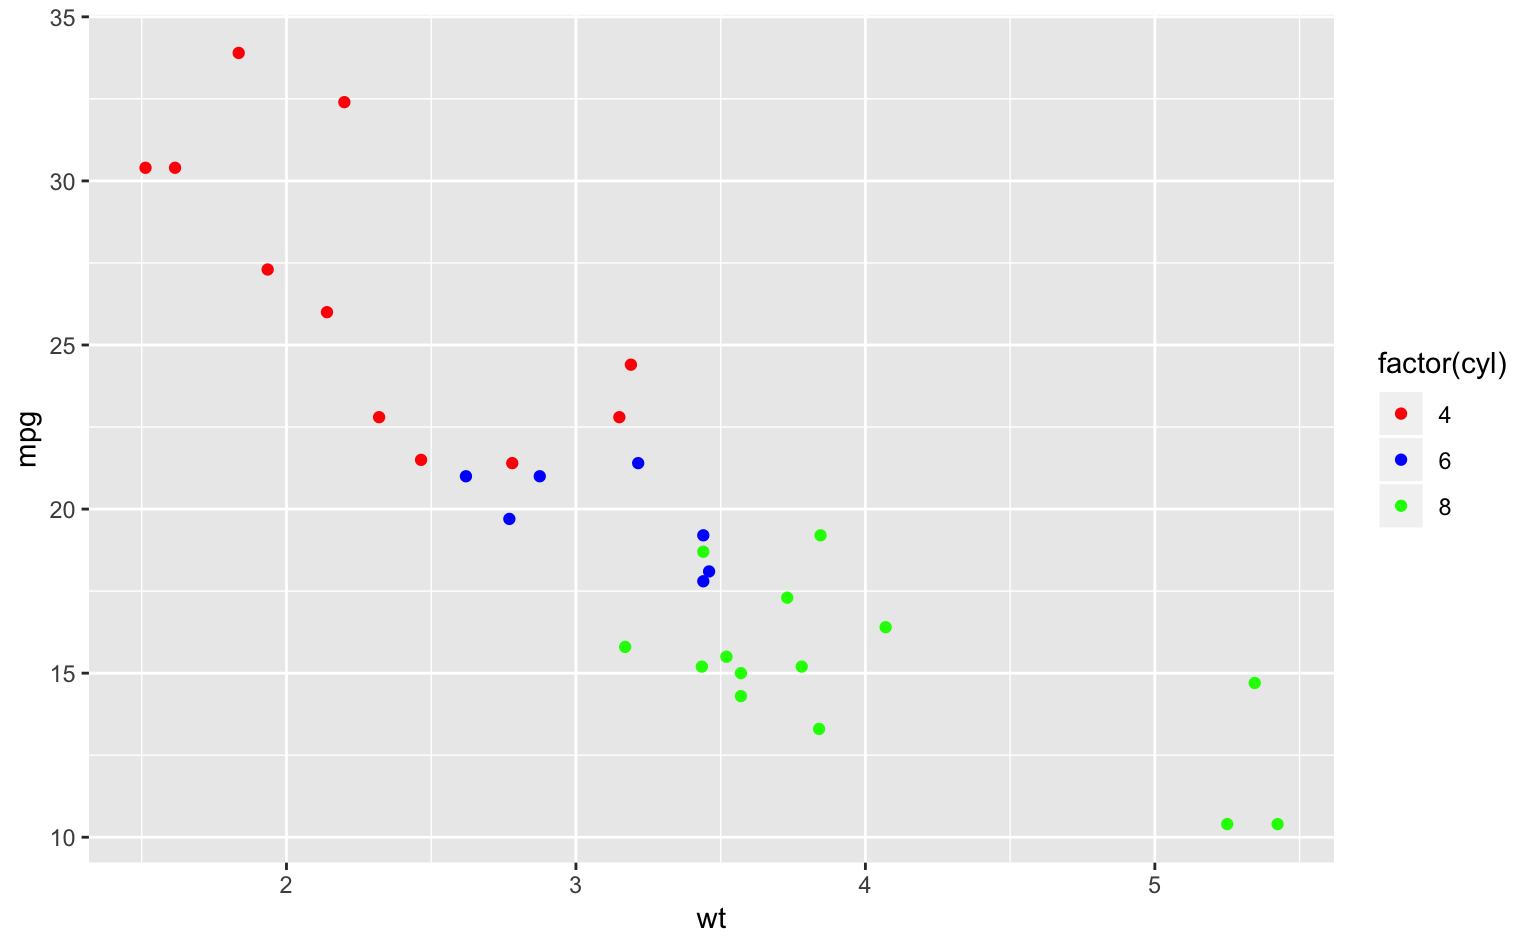
\includegraphics{lecture_note_files/figure-latex/color-1-1} 

}

\caption{\texttt{scale\_color\_manual()}によって色を変えたグラフ。}\label{fig:color-1}
\end{figure}

ggplot2には、他にも色や見た目を調整するための様々な関数がある。また、色の調整にはcolorspaceというパッケージが便利だが、本資料はあくまで最低限のレベルの可視化について解説するものなので、ここではあまり深く突っ込まないことにする\footnote{ここまでついてこれた人であれば、自力で検索してマスターできるだろう(たぶん)。}。

\section{軸}

デフォルトの設定だと、変数名がそのまま軸のラベルになってしまう。データを探索的に分析(\textbf{data
exploration})している最中はそれで問題ないかもしれない。しかし、内容を他の人と共有(\textbf{data
presentation})したい場合は、なるべくわかりやすくするため、軸名を変えるなどの調整が必要になるだろう\footnote{気配りと言うほどのものでもないが、こういうことをやるかやらないかで、ゼミメンバーや聴衆が自分の話を聞く態度は変わってくるだろう(たぶん)。}。

グラフの軸ラベルは\texttt{labs()}という関数で一括変更することができる。なお、下では具体例として\texttt{Title}や\texttt{Subtitle}なども指定しているが、実用上はごちゃごちゃしてしまうだけなので、基本的には指定しなくても良い。

(ref:label-1)
\texttt{labs()}を使い、軸名をデフォルトから変更したグラフ。

\begin{Shaded}
\begin{Highlighting}[]
\KeywordTok{ggplot}\NormalTok{(mtcars, }\KeywordTok{aes}\NormalTok{(wt, mpg, }\DataTypeTok{color =} \KeywordTok{factor}\NormalTok{(cyl))) }\OperatorTok{+}
\StringTok{  }\KeywordTok{geom_point}\NormalTok{() }\OperatorTok{+}
\StringTok{  }\KeywordTok{labs}\NormalTok{(}\DataTypeTok{x =} \StringTok{"Weight (1,000 Ibs)"}\NormalTok{,}
       \DataTypeTok{y =} \StringTok{"Miles/(US) gallon"}\NormalTok{,}
       \DataTypeTok{title =} \StringTok{"Title"}\NormalTok{,}
       \DataTypeTok{subtitle =} \StringTok{"Subtitle"}\NormalTok{,}
       \DataTypeTok{caption =} \StringTok{"Caption"}\NormalTok{,}
       \DataTypeTok{tag =} \StringTok{"Tag"}\NormalTok{)}
\end{Highlighting}
\end{Shaded}

\begin{figure}

{\centering \includegraphics{lecture_note_files/figure-latex/unnamed-chunk-95-1} 

}

\caption{(ref:label-1)}\label{fig:unnamed-chunk-95}
\end{figure}

\section{凡例}

ここでは、凡例を「消す」方法を解説する。なぜなら、グラフに凡例がなくとも自明な場合も多いからである。下の図はFigure
\ref{fig:boxplot-1}の凡例を消したグラフである。



\begin{Shaded}
\begin{Highlighting}[]
\KeywordTok{ggplot}\NormalTok{(PlantGrowth, }\KeywordTok{aes}\NormalTok{(group, weight, }\DataTypeTok{fill =}\NormalTok{ group)) }\OperatorTok{+}\StringTok{ }\CommentTok{# x軸にgroup、y軸にweight;fillで色の塗りつぶし}
\StringTok{  }\KeywordTok{geom_boxplot}\NormalTok{() }\OperatorTok{+}\StringTok{ }\CommentTok{# 箱ひげ図}
\StringTok{  }\KeywordTok{guides}\NormalTok{(}\DataTypeTok{fill =} \OtherTok{FALSE}\NormalTok{) }\CommentTok{# 凡例(ここではfill)を消すためのコード}
\end{Highlighting}
\end{Shaded}

\begin{figure}

{\centering \includegraphics{lecture_note_files/figure-latex/legend-1-1} 

}

\caption{凡例を消したグラフ。}\label{fig:legend-1}
\end{figure}

\section{複数パネルのグラフ}

論文などを描く際、複数個のグラフを組み合わせて1枚のグラフにしたいことがある。そのときは、patchworkパッケージを使うと良い。patchworkは以下の手順でインストールする。

\begin{Shaded}
\begin{Highlighting}[]
\KeywordTok{library}\NormalTok{(devtools)}
\KeywordTok{install_github}\NormalTok{(}\StringTok{"thomasp85/patchwork"}\NormalTok{) }\CommentTok{# パッケージのインストール}
\end{Highlighting}
\end{Shaded}

\begin{Shaded}
\begin{Highlighting}[]
\KeywordTok{library}\NormalTok{(patchwork) }\CommentTok{# パッケージの読み込み}
\end{Highlighting}
\end{Shaded}

patchworkを使うと、たとえば下のように、複数のパネルを直観的に組み合わせることができる。



\begin{Shaded}
\begin{Highlighting}[]
\CommentTok{# まずパネルa(panel_a)を作る}
\NormalTok{panel_a =}\StringTok{ }\KeywordTok{ggplot}\NormalTok{(mtcars, }\KeywordTok{aes}\NormalTok{(wt, mpg, }\DataTypeTok{color =} \KeywordTok{factor}\NormalTok{(cyl))) }\OperatorTok{+}
\StringTok{  }\KeywordTok{geom_point}\NormalTok{()}

\CommentTok{# 次にパネルb(panel_b)を作る}
\NormalTok{panel_b =}\StringTok{ }\KeywordTok{ggplot}\NormalTok{(mtcars, }\KeywordTok{aes}\NormalTok{(wt, disp, }\DataTypeTok{color =} \KeywordTok{factor}\NormalTok{(cyl))) }\OperatorTok{+}
\StringTok{  }\KeywordTok{geom_point}\NormalTok{()}

\CommentTok{# 2つを足し算して1枚のグラフ(panel_ab)にし、1列に並べる(ncol = 1)}
\NormalTok{panel_ab =}\StringTok{ }\NormalTok{panel_a }\OperatorTok{+}\StringTok{ }\NormalTok{panel_b }\OperatorTok{+}\StringTok{ }
\StringTok{  }\KeywordTok{plot_layout}\NormalTok{(}\DataTypeTok{ncol =} \DecValTok{1}\NormalTok{) }\OperatorTok{+}\StringTok{ }
\StringTok{  }\KeywordTok{plot_annotation}\NormalTok{(}\DataTypeTok{tag_levels =} \StringTok{"a"}\NormalTok{) }\CommentTok{# 最後にタグを付ける}

\NormalTok{panel_ab}
\end{Highlighting}
\end{Shaded}

\begin{figure}

{\centering \includegraphics{lecture_note_files/figure-latex/unnamed-chunk-98-1} 

}

\caption{2枚のパネルを組み合わせたグラフ。}\label{fig:unnamed-chunk-98}
\end{figure}

\section{グラフの保存}

論文にグラフを貼り付ける前に、当然グラフを画像ファイルとして保存しなければならない。上で作った\texttt{panel\_ab}を``panel\_ab.pdf''として保存してみよう。グラフは\texttt{ggsave("保存するファイル名",\ plot\ =\ グラフのオブジェクト,\ width\ =\ 幅,\ height\ =\ 高さ,\ units\ =\ "サイズの単位")}で保存することができる。

\begin{Shaded}
\begin{Highlighting}[]
\KeywordTok{ggsave}\NormalTok{(}\StringTok{"panel_ab.pdf"}\NormalTok{, }\DataTypeTok{plot =}\NormalTok{ panel_ab, }\DataTypeTok{width =} \DecValTok{14}\NormalTok{, }\DataTypeTok{height =} \DecValTok{14}\NormalTok{, }\DataTypeTok{units =} \StringTok{"cm"}\NormalTok{)}
\end{Highlighting}
\end{Shaded}

なお、余程のことがない限り、グラフは基本的にPDF形式で保存するのが良い\footnote{PDF形式で保存する場合、色々面倒なことが起こるかもしれないが、そこら辺はググって解決しよう。}。なぜPDFが良いのかはGoogle先生が教えてくれるだろう。

\section{練習問題}\label{-5}

\begin{itemize}
\tightlist
\item
  gcookbookの\texttt{heightweight}データを使い、性別ごとにパネルを分けた上で、身長と体重の散布図を描いてみよう。また、凡例を消し、軸ラベルをわかりやすく書き直してみよう(日本語だとうまく表示されない可能性があるので、英語で良い)。余力があれば、各パネル(サブプロット)のラベルも書き直してみよう。
\end{itemize}

\part*{データハンドリング}\label{part-}
\addcontentsline{toc}{part}{データハンドリング}

\chapter{データハンドリング}\label{data-handling}

ここまで、ggplot2を使ったデータの可視化を見てきた。ただし、ggplot2で作図をする際、大きな前提条件がある。それは、\textbf{データを行列(データフレームもしくはtibbleと呼ばれる形式)で用意しなければいけない}というものである。つまり、変数を列に、観測値を行に取るようなデータ構造にあらかじめ整形しなければならないということである。

たとえば、今まで使ってきた\texttt{mtcars}、\texttt{faithful}のデータ構造を改めて見てみよう。

\begin{Shaded}
\begin{Highlighting}[]
\KeywordTok{head}\NormalTok{(mtcars) }\CommentTok{# 先頭6行}
\end{Highlighting}
\end{Shaded}

\begin{verbatim}
##                    mpg cyl disp  hp drat    wt  qsec vs am gear carb
## Mazda RX4         21.0   6  160 110 3.90 2.620 16.46  0  1    4    4
## Mazda RX4 Wag     21.0   6  160 110 3.90 2.875 17.02  0  1    4    4
## Datsun 710        22.8   4  108  93 3.85 2.320 18.61  1  1    4    1
## Hornet 4 Drive    21.4   6  258 110 3.08 3.215 19.44  1  0    3    1
## Hornet Sportabout 18.7   8  360 175 3.15 3.440 17.02  0  0    3    2
## Valiant           18.1   6  225 105 2.76 3.460 20.22  1  0    3    1
\end{verbatim}

\begin{Shaded}
\begin{Highlighting}[]
\KeywordTok{head}\NormalTok{(faithful) }\CommentTok{# 先頭6行}
\end{Highlighting}
\end{Shaded}

\begin{verbatim}
##   eruptions waiting
## 1     3.600      79
## 2     1.800      54
## 3     3.333      74
## 4     2.283      62
## 5     4.533      85
## 6     2.883      55
\end{verbatim}

どちらも、列に変数名、行に観測値という構造になっている。

\begin{center}\rule{0.5\linewidth}{\linethickness}\end{center}

散布図、箱ひげ図、ヒストグラムのように、これらのデータの素値をプロットする際、データハンドリングはあまり問題にならない。しかし、実際は平均値や標準誤差のように、何かしらの統計的処理を施した値をプロットしたいこともある。また、ある1つのグループのデータだけをプロットしたいという場合もある。

可視化の際に直面する問題は、おおよそ以下の3つに大別できるだろう。

\begin{itemize}
\item
  \textbf{1つのグループのデータだけを抽出した上でプロットしたい}(たとえば、3条件のうち統制条件だけプロットしたい、など)
\item
  \textbf{素値ではなく、平均値や標準誤差などの統計量をプロットしたい}
\item
  \textbf{2つ以上のデータフレームを結合してプロットしたい}
\end{itemize}

などである。これらの問題は、いずれも\textbf{tidyverse}と呼ばれるパッケージ群を使えば解決する。

\section{tidyverse}\label{tidyverse}

データハンドリングに使うパッケージ群(複数のパッケージ)はtidyverseと呼ばれており、\texttt{library(tidyverse)}で読み込むことができる。ちなみにggplot2もtidyverseの一部なので、自動的に読み込まれる。下のコードを実行すると色々メッセージが出るかもしれないが、気にしなくて良い。

\begin{Shaded}
\begin{Highlighting}[]
\KeywordTok{library}\NormalTok{(tidyverse) }\CommentTok{# データハンドリング用のパッケージおよびggplot2を読み込む}
\end{Highlighting}
\end{Shaded}

この章では、主にggplot2の\texttt{mpg}(自動車のデータ)を使い、データハンドリングを見ていくことにする。

\section{抽出}

\subsection{データの値で絞り込み}

データの値によって絞り込みを行いたい時がある。たとえば、\texttt{mpg}であれば、\texttt{manufacturer}の種類でデータを絞り込みたい(データの行単位で抽出したい)ということである。心理学の実験データで言えば、男性/女性のデータのみ抽出したいというような場面を想像してみてほしい。

このようなときは、\texttt{filter(抽出条件)}を使えば良い。

\begin{Shaded}
\begin{Highlighting}[]
\NormalTok{mpg }\OperatorTok
\StringTok{  }\KeywordTok{filter}\NormalTok{(manufacturer }\OperatorTok{==}\StringTok{ "audi"}\NormalTok{) }\CommentTok{# manufacturerが"audi"のものだけを抽出}
\end{Highlighting}
\end{Shaded}

\begin{verbatim}
## # A tibble: 18 x 11
##    manufacturer model      displ  year   cyl trans      drv     cty   hwy
##    <chr>        <chr>      <dbl> <int> <int> <chr>      <chr> <int> <int>
##  1 audi         a4           1.8  1999     4 auto(l5)   f        18    29
##  2 audi         a4           1.8  1999     4 manual(m5) f        21    29
##  3 audi         a4           2    2008     4 manual(m6) f        20    31
##  4 audi         a4           2    2008     4 auto(av)   f        21    30
##  5 audi         a4           2.8  1999     6 auto(l5)   f        16    26
##  6 audi         a4           2.8  1999     6 manual(m5) f        18    26
##  7 audi         a4           3.1  2008     6 auto(av)   f        18    27
##  8 audi         a4 quattro   1.8  1999     4 manual(m5) 4        18    26
##  9 audi         a4 quattro   1.8  1999     4 auto(l5)   4        16    25
## 10 audi         a4 quattro   2    2008     4 manual(m6) 4        20    28
## 11 audi         a4 quattro   2    2008     4 auto(s6)   4        19    27
## 12 audi         a4 quattro   2.8  1999     6 auto(l5)   4        15    25
## 13 audi         a4 quattro   2.8  1999     6 manual(m5) 4        17    25
## 14 audi         a4 quattro   3.1  2008     6 auto(s6)   4        17    25
## 15 audi         a4 quattro   3.1  2008     6 manual(m6) 4        15    25
## 16 audi         a6 quattro   2.8  1999     6 auto(l5)   4        15    24
## 17 audi         a6 quattro   3.1  2008     6 auto(s6)   4        17    25
## 18 audi         a6 quattro   4.2  2008     8 auto(s6)   4        16    23
##    fl    class  
##    <chr> <chr>  
##  1 p     compact
##  2 p     compact
##  3 p     compact
##  4 p     compact
##  5 p     compact
##  6 p     compact
##  7 p     compact
##  8 p     compact
##  9 p     compact
## 10 p     compact
## 11 p     compact
## 12 p     compact
## 13 p     compact
## 14 p     compact
## 15 p     compact
## 16 p     midsize
## 17 p     midsize
## 18 p     midsize
\end{verbatim}

ここで、\texttt{==}は「等しい」ということを意味している。大体のプログラミング言語では、\texttt{==}は「等しい」を、\texttt{=}は「代入する」を意味することに注意しよう。

ちなみに、\texttt{\%\textgreater{}\%}はパイプ演算子と呼ばれており、オブジェクトを次の関数の第一引数に突っ込むという操作を表している。ちょっと何を言っているのか分からないと思うが、あまり気にしなくて良い。上のコードで何がおこなわれているのか、少なくとも直観的には分かるだろう。今はそれで大丈夫である。

\begin{center}\rule{0.5\linewidth}{\linethickness}\end{center}

複数条件で絞り込むこともできる。たとえば、「\texttt{manufacturer}が\texttt{"audi"}」\textbf{かつ}「\texttt{model}が\texttt{"a4"}」の行を抽出したい場合は、条件を\texttt{\&}で繋げば良い。

\begin{Shaded}
\begin{Highlighting}[]
\NormalTok{mpg }\OperatorTok
\StringTok{  }\KeywordTok{filter}\NormalTok{(manufacturer }\OperatorTok{==}\StringTok{ "audi"} \OperatorTok{&}\StringTok{ }\NormalTok{model }\OperatorTok{==}\StringTok{ "a4"}\NormalTok{)}
\end{Highlighting}
\end{Shaded}

\begin{verbatim}
## # A tibble: 7 x 11
##   manufacturer model displ  year   cyl trans      drv     cty   hwy fl   
##   <chr>        <chr> <dbl> <int> <int> <chr>      <chr> <int> <int> <chr>
## 1 audi         a4      1.8  1999     4 auto(l5)   f        18    29 p    
## 2 audi         a4      1.8  1999     4 manual(m5) f        21    29 p    
## 3 audi         a4      2    2008     4 manual(m6) f        20    31 p    
## 4 audi         a4      2    2008     4 auto(av)   f        21    30 p    
## 5 audi         a4      2.8  1999     6 auto(l5)   f        16    26 p    
## 6 audi         a4      2.8  1999     6 manual(m5) f        18    26 p    
## 7 audi         a4      3.1  2008     6 auto(av)   f        18    27 p    
##   class  
##   <chr>  
## 1 compact
## 2 compact
## 3 compact
## 4 compact
## 5 compact
## 6 compact
## 7 compact
\end{verbatim}

「\texttt{manufacturer}が\texttt{"audi"}」\textbf{または}「\texttt{model}が\texttt{"a4"}」の行を抽出したい場合は、条件を\texttt{\textbar{}}で繋げば良い。

\begin{Shaded}
\begin{Highlighting}[]
\NormalTok{mpg }\OperatorTok
\StringTok{  }\KeywordTok{filter}\NormalTok{(manufacturer }\OperatorTok{==}\StringTok{ "audi"} \OperatorTok{|}\StringTok{ }\NormalTok{model }\OperatorTok{==}\StringTok{ "a4"}\NormalTok{)}
\end{Highlighting}
\end{Shaded}

\begin{verbatim}
## # A tibble: 18 x 11
##    manufacturer model      displ  year   cyl trans      drv     cty   hwy
##    <chr>        <chr>      <dbl> <int> <int> <chr>      <chr> <int> <int>
##  1 audi         a4           1.8  1999     4 auto(l5)   f        18    29
##  2 audi         a4           1.8  1999     4 manual(m5) f        21    29
##  3 audi         a4           2    2008     4 manual(m6) f        20    31
##  4 audi         a4           2    2008     4 auto(av)   f        21    30
##  5 audi         a4           2.8  1999     6 auto(l5)   f        16    26
##  6 audi         a4           2.8  1999     6 manual(m5) f        18    26
##  7 audi         a4           3.1  2008     6 auto(av)   f        18    27
##  8 audi         a4 quattro   1.8  1999     4 manual(m5) 4        18    26
##  9 audi         a4 quattro   1.8  1999     4 auto(l5)   4        16    25
## 10 audi         a4 quattro   2    2008     4 manual(m6) 4        20    28
## 11 audi         a4 quattro   2    2008     4 auto(s6)   4        19    27
## 12 audi         a4 quattro   2.8  1999     6 auto(l5)   4        15    25
## 13 audi         a4 quattro   2.8  1999     6 manual(m5) 4        17    25
## 14 audi         a4 quattro   3.1  2008     6 auto(s6)   4        17    25
## 15 audi         a4 quattro   3.1  2008     6 manual(m6) 4        15    25
## 16 audi         a6 quattro   2.8  1999     6 auto(l5)   4        15    24
## 17 audi         a6 quattro   3.1  2008     6 auto(s6)   4        17    25
## 18 audi         a6 quattro   4.2  2008     8 auto(s6)   4        16    23
##    fl    class  
##    <chr> <chr>  
##  1 p     compact
##  2 p     compact
##  3 p     compact
##  4 p     compact
##  5 p     compact
##  6 p     compact
##  7 p     compact
##  8 p     compact
##  9 p     compact
## 10 p     compact
## 11 p     compact
## 12 p     compact
## 13 p     compact
## 14 p     compact
## 15 p     compact
## 16 p     midsize
## 17 p     midsize
## 18 p     midsize
\end{verbatim}

「\texttt{manufacturer}が\texttt{"audi"}」\textbf{でもなく}「\texttt{model}が\texttt{"a4"}」\textbf{でもない}行を抽出したい場合は、条件を\texttt{!()}で囲めば良い。\texttt{!()}は論理値を反転させる演算子である\footnote{ちなみに「\texttt{manufacturer}が\texttt{"audi"}ではない」を書きたいときは、\texttt{manufacturer\ !=\ "audi"}とすれば良い。}。

\begin{Shaded}
\begin{Highlighting}[]
\NormalTok{mpg }\OperatorTok
\StringTok{  }\KeywordTok{filter}\NormalTok{(}\OperatorTok{!}\NormalTok{(manufacturer }\OperatorTok{==}\StringTok{ "audi"} \OperatorTok{|}\StringTok{ }\NormalTok{model }\OperatorTok{==}\StringTok{ "a4"}\NormalTok{))}
\end{Highlighting}
\end{Shaded}

\begin{verbatim}
## # A tibble: 216 x 11
##    manufacturer model              displ  year   cyl trans      drv     cty
##    <chr>        <chr>              <dbl> <int> <int> <chr>      <chr> <int>
##  1 chevrolet    c1500 suburban 2wd   5.3  2008     8 auto(l4)   r        14
##  2 chevrolet    c1500 suburban 2wd   5.3  2008     8 auto(l4)   r        11
##  3 chevrolet    c1500 suburban 2wd   5.3  2008     8 auto(l4)   r        14
##  4 chevrolet    c1500 suburban 2wd   5.7  1999     8 auto(l4)   r        13
##  5 chevrolet    c1500 suburban 2wd   6    2008     8 auto(l4)   r        12
##  6 chevrolet    corvette             5.7  1999     8 manual(m6) r        16
##  7 chevrolet    corvette             5.7  1999     8 auto(l4)   r        15
##  8 chevrolet    corvette             6.2  2008     8 manual(m6) r        16
##  9 chevrolet    corvette             6.2  2008     8 auto(s6)   r        15
## 10 chevrolet    corvette             7    2008     8 manual(m6) r        15
##      hwy fl    class  
##    <int> <chr> <chr>  
##  1    20 r     suv    
##  2    15 e     suv    
##  3    20 r     suv    
##  4    17 r     suv    
##  5    17 r     suv    
##  6    26 p     2seater
##  7    23 p     2seater
##  8    26 p     2seater
##  9    25 p     2seater
## 10    24 p     2seater
## # ... with 206 more rows
\end{verbatim}

\subsection{データの列で絞り込み}

では、列方向で抽出するにはどうすれば良いのだろうか? たとえば、\texttt{mpg}で言えば、\texttt{manufacturer}と\texttt{model}と\texttt{trans}と\texttt{drv}の列を抽出したいというような状況である。

このようなときは、\texttt{select(抽出したい列名)}を使えば良い。抽出したい列名は、1つだけに限らず、何個書いても問題ない。

\begin{Shaded}
\begin{Highlighting}[]
\NormalTok{mpg }\OperatorTok
\StringTok{  }\KeywordTok{select}\NormalTok{(manufacturer, model, trans, drv) }\CommentTok{# 4つの列を抽出}
\end{Highlighting}
\end{Shaded}

\begin{verbatim}
## # A tibble: 234 x 4
##    manufacturer model      trans      drv  
##    <chr>        <chr>      <chr>      <chr>
##  1 audi         a4         auto(l5)   f    
##  2 audi         a4         manual(m5) f    
##  3 audi         a4         manual(m6) f    
##  4 audi         a4         auto(av)   f    
##  5 audi         a4         auto(l5)   f    
##  6 audi         a4         manual(m5) f    
##  7 audi         a4         auto(av)   f    
##  8 audi         a4 quattro manual(m5) 4    
##  9 audi         a4 quattro auto(l5)   4    
## 10 audi         a4 quattro manual(m6) 4    
## # ... with 224 more rows
\end{verbatim}

\texttt{select()}では、「A列からG列まで」というような抽出も可能である。

\begin{Shaded}
\begin{Highlighting}[]
\NormalTok{mpg }\OperatorTok
\StringTok{  }\KeywordTok{select}\NormalTok{(manufacturer}\OperatorTok{:}\NormalTok{drv) }\CommentTok{# manufacturerからdrvまでの7列を抽出}
\end{Highlighting}
\end{Shaded}

\begin{verbatim}
## # A tibble: 234 x 7
##    manufacturer model      displ  year   cyl trans      drv  
##    <chr>        <chr>      <dbl> <int> <int> <chr>      <chr>
##  1 audi         a4           1.8  1999     4 auto(l5)   f    
##  2 audi         a4           1.8  1999     4 manual(m5) f    
##  3 audi         a4           2    2008     4 manual(m6) f    
##  4 audi         a4           2    2008     4 auto(av)   f    
##  5 audi         a4           2.8  1999     6 auto(l5)   f    
##  6 audi         a4           2.8  1999     6 manual(m5) f    
##  7 audi         a4           3.1  2008     6 auto(av)   f    
##  8 audi         a4 quattro   1.8  1999     4 manual(m5) 4    
##  9 audi         a4 quattro   1.8  1999     4 auto(l5)   4    
## 10 audi         a4 quattro   2    2008     4 manual(m6) 4    
## # ... with 224 more rows
\end{verbatim}

\texttt{select(-列名)}とすれば、指定した列を除外することもできる。

\begin{Shaded}
\begin{Highlighting}[]
\NormalTok{mpg }\OperatorTok
\StringTok{  }\KeywordTok{select}\NormalTok{(}\OperatorTok{-}\NormalTok{manufacturer) }\CommentTok{# manufacturerを除外}
\end{Highlighting}
\end{Shaded}

\begin{verbatim}
## # A tibble: 234 x 10
##    model      displ  year   cyl trans      drv     cty   hwy fl    class  
##    <chr>      <dbl> <int> <int> <chr>      <chr> <int> <int> <chr> <chr>  
##  1 a4           1.8  1999     4 auto(l5)   f        18    29 p     compact
##  2 a4           1.8  1999     4 manual(m5) f        21    29 p     compact
##  3 a4           2    2008     4 manual(m6) f        20    31 p     compact
##  4 a4           2    2008     4 auto(av)   f        21    30 p     compact
##  5 a4           2.8  1999     6 auto(l5)   f        16    26 p     compact
##  6 a4           2.8  1999     6 manual(m5) f        18    26 p     compact
##  7 a4           3.1  2008     6 auto(av)   f        18    27 p     compact
##  8 a4 quattro   1.8  1999     4 manual(m5) 4        18    26 p     compact
##  9 a4 quattro   1.8  1999     4 auto(l5)   4        16    25 p     compact
## 10 a4 quattro   2    2008     4 manual(m6) 4        20    28 p     compact
## # ... with 224 more rows
\end{verbatim}

\section{追加}

\subsection{新しい列を追加}

データフレームに新しい列を作るには、\texttt{mutate(新しく作る列名\ =\ 値)}を使えば良い。

\begin{Shaded}
\begin{Highlighting}[]
\NormalTok{mpg }\OperatorTok
\StringTok{  }\KeywordTok{mutate}\NormalTok{(}\DataTypeTok{one =} \DecValTok{1}\NormalTok{) }\CommentTok{# 最後尾にoneという列を追加した}
\end{Highlighting}
\end{Shaded}

\begin{verbatim}
## # A tibble: 234 x 12
##    manufacturer model      displ  year   cyl trans      drv     cty   hwy
##    <chr>        <chr>      <dbl> <int> <int> <chr>      <chr> <int> <int>
##  1 audi         a4           1.8  1999     4 auto(l5)   f        18    29
##  2 audi         a4           1.8  1999     4 manual(m5) f        21    29
##  3 audi         a4           2    2008     4 manual(m6) f        20    31
##  4 audi         a4           2    2008     4 auto(av)   f        21    30
##  5 audi         a4           2.8  1999     6 auto(l5)   f        16    26
##  6 audi         a4           2.8  1999     6 manual(m5) f        18    26
##  7 audi         a4           3.1  2008     6 auto(av)   f        18    27
##  8 audi         a4 quattro   1.8  1999     4 manual(m5) 4        18    26
##  9 audi         a4 quattro   1.8  1999     4 auto(l5)   4        16    25
## 10 audi         a4 quattro   2    2008     4 manual(m6) 4        20    28
##    fl    class     one
##    <chr> <chr>   <dbl>
##  1 p     compact     1
##  2 p     compact     1
##  3 p     compact     1
##  4 p     compact     1
##  5 p     compact     1
##  6 p     compact     1
##  7 p     compact     1
##  8 p     compact     1
##  9 p     compact     1
## 10 p     compact     1
## # ... with 224 more rows
\end{verbatim}

上の例では\texttt{one}という列を作り、すべての行を1で埋めたが、これはあまり実践的ではない。

\texttt{mutate()}が力を発揮するのは、特に\texttt{if\_else()}という関数と組み合わせたときである。たとえば、\texttt{displ}(排気量)の値が3未満なら\texttt{good}、3以上なら\texttt{bad}という列(\texttt{engine})を作りたい場合、以下のように書けば良い。

\begin{Shaded}
\begin{Highlighting}[]
\NormalTok{mpg }\OperatorTok
\StringTok{  }\KeywordTok{mutate}\NormalTok{(}\DataTypeTok{engine =} \KeywordTok{if_else}\NormalTok{(displ }\OperatorTok{<}\StringTok{ }\DecValTok{3}\NormalTok{, }\StringTok{"good"}\NormalTok{, }\StringTok{"bad"}\NormalTok{))}
\end{Highlighting}
\end{Shaded}

\begin{verbatim}
## # A tibble: 234 x 12
##    manufacturer model      displ  year   cyl trans      drv     cty   hwy
##    <chr>        <chr>      <dbl> <int> <int> <chr>      <chr> <int> <int>
##  1 audi         a4           1.8  1999     4 auto(l5)   f        18    29
##  2 audi         a4           1.8  1999     4 manual(m5) f        21    29
##  3 audi         a4           2    2008     4 manual(m6) f        20    31
##  4 audi         a4           2    2008     4 auto(av)   f        21    30
##  5 audi         a4           2.8  1999     6 auto(l5)   f        16    26
##  6 audi         a4           2.8  1999     6 manual(m5) f        18    26
##  7 audi         a4           3.1  2008     6 auto(av)   f        18    27
##  8 audi         a4 quattro   1.8  1999     4 manual(m5) 4        18    26
##  9 audi         a4 quattro   1.8  1999     4 auto(l5)   4        16    25
## 10 audi         a4 quattro   2    2008     4 manual(m6) 4        20    28
##    fl    class   engine
##    <chr> <chr>   <chr> 
##  1 p     compact good  
##  2 p     compact good  
##  3 p     compact good  
##  4 p     compact good  
##  5 p     compact good  
##  6 p     compact good  
##  7 p     compact bad   
##  8 p     compact good  
##  9 p     compact good  
## 10 p     compact good  
## # ... with 224 more rows
\end{verbatim}

\subsection{列名を変更}

新しい列を作りたいわけではないが、列名を変えたい場合がある。このようなときは、\texttt{rename(新しい列名\ =\ 古い列名)}を使えば良い。

\begin{Shaded}
\begin{Highlighting}[]
\NormalTok{mpg }\OperatorTok
\StringTok{  }\KeywordTok{rename}\NormalTok{(}\DataTypeTok{nen =}\NormalTok{ year) }\CommentTok{# yearをnenに変更}
\end{Highlighting}
\end{Shaded}

\begin{verbatim}
## # A tibble: 234 x 11
##    manufacturer model      displ   nen   cyl trans      drv     cty   hwy
##    <chr>        <chr>      <dbl> <int> <int> <chr>      <chr> <int> <int>
##  1 audi         a4           1.8  1999     4 auto(l5)   f        18    29
##  2 audi         a4           1.8  1999     4 manual(m5) f        21    29
##  3 audi         a4           2    2008     4 manual(m6) f        20    31
##  4 audi         a4           2    2008     4 auto(av)   f        21    30
##  5 audi         a4           2.8  1999     6 auto(l5)   f        16    26
##  6 audi         a4           2.8  1999     6 manual(m5) f        18    26
##  7 audi         a4           3.1  2008     6 auto(av)   f        18    27
##  8 audi         a4 quattro   1.8  1999     4 manual(m5) 4        18    26
##  9 audi         a4 quattro   1.8  1999     4 auto(l5)   4        16    25
## 10 audi         a4 quattro   2    2008     4 manual(m6) 4        20    28
##    fl    class  
##    <chr> <chr>  
##  1 p     compact
##  2 p     compact
##  3 p     compact
##  4 p     compact
##  5 p     compact
##  6 p     compact
##  7 p     compact
##  8 p     compact
##  9 p     compact
## 10 p     compact
## # ... with 224 more rows
\end{verbatim}

\section{集約}

統計量の算出に使えるのは、\texttt{group\_by()}と\texttt{summarise()}である。

まずは\texttt{summarise()}を見てみよう。書き方は\texttt{summarise(新しい列名\ =\ 関数)}である。同時に複数の関数を使うこともできる。たとえば、\texttt{displ}の平均値、標準偏差、最小値、最大値を計算したい場合、以下のように書けば良い。

\begin{Shaded}
\begin{Highlighting}[]
\NormalTok{mpg }\OperatorTok
\StringTok{  }\KeywordTok{summarise}\NormalTok{(}\DataTypeTok{mean_displ =} \KeywordTok{mean}\NormalTok{(displ),}
            \DataTypeTok{sd_displ =} \KeywordTok{sd}\NormalTok{(displ),}
            \DataTypeTok{min_displ =} \KeywordTok{min}\NormalTok{(displ),}
            \DataTypeTok{max_displ =} \KeywordTok{max}\NormalTok{(displ))}
\end{Highlighting}
\end{Shaded}

\begin{verbatim}
## # A tibble: 1 x 4
##   mean_displ sd_displ min_displ max_displ
##        <dbl>    <dbl>     <dbl>     <dbl>
## 1       3.47     1.29       1.6         7
\end{verbatim}

このように、\texttt{summarise()}を使うと、データ全体の統計量を計算することができる。

\begin{center}\rule{0.5\linewidth}{\linethickness}\end{center}

しかし、実際の場面で全体の統計量を計算することは少なく、むしろグループごとの統計量を計算したいという場面のほうが圧倒的に多いだろう。

このようなときは、\texttt{group\_by(グルーピングの変数)}を使うことができる。たとえば、\texttt{year}ごとに\texttt{summarise()}を実行するには、以下のように書けば良い。

\begin{Shaded}
\begin{Highlighting}[]
\NormalTok{mpg }\OperatorTok
\StringTok{  }\KeywordTok{group_by}\NormalTok{(year) }\OperatorTok
\StringTok{  }\KeywordTok{summarise}\NormalTok{(}\DataTypeTok{mean_displ =} \KeywordTok{mean}\NormalTok{(displ),}
            \DataTypeTok{sd_displ =} \KeywordTok{sd}\NormalTok{(displ),}
            \DataTypeTok{min_displ =} \KeywordTok{min}\NormalTok{(displ),}
            \DataTypeTok{max_displ =} \KeywordTok{max}\NormalTok{(displ))}
\end{Highlighting}
\end{Shaded}

\begin{verbatim}
## # A tibble: 2 x 5
##    year mean_displ sd_displ min_displ max_displ
##   <int>      <dbl>    <dbl>     <dbl>     <dbl>
## 1  1999       3.28     1.26       1.6       6.5
## 2  2008       3.66     1.30       1.8       7
\end{verbatim}

製造年(1999年と2008年)ごとに統計量を計算することができた。

\section{結合}

ここでは、\texttt{mpg}ではなく、架空のデータセットを作ってみよう。たとえば、以下のような状況を考えてみてほしい。

\begin{quote}
たかし君とはなこさんは、以前見たテレビドラマに感化されて、「足袋を履いたときと、裸足のときとで、どっちが走るのが早くなるだろうか?」と疑問に思いました。そこで2人は、5日間のうち3日は足袋を履いて、2日は裸足で自宅から学校まで走り、到着までの所要時間を測りました。
\end{quote}

2人の毎日の所要時間データは\texttt{commute}というデータフレームとして保存しよう。

\begin{Shaded}
\begin{Highlighting}[]
\NormalTok{commute =}\StringTok{ }\KeywordTok{data.frame}\NormalTok{(}
  \StringTok{"name"}\NormalTok{ =}\StringTok{ }\KeywordTok{c}\NormalTok{(}\StringTok{"takashi"}\NormalTok{,}\StringTok{"takashi"}\NormalTok{,}\StringTok{"takashi"}\NormalTok{,}\StringTok{"takashi"}\NormalTok{,}\StringTok{"takashi"}\NormalTok{,}\StringTok{"hanako"}\NormalTok{,}\StringTok{"hanako"}\NormalTok{,}\StringTok{"hanako"}\NormalTok{,}\StringTok{"hanako"}\NormalTok{,}\StringTok{"hanako"}\NormalTok{),}
  \StringTok{"day"}\NormalTok{ =}\StringTok{ }\KeywordTok{c}\NormalTok{(}\DecValTok{1}\NormalTok{,}\DecValTok{2}\NormalTok{,}\DecValTok{3}\NormalTok{,}\DecValTok{4}\NormalTok{,}\DecValTok{5}\NormalTok{,}\DecValTok{1}\NormalTok{,}\DecValTok{2}\NormalTok{,}\DecValTok{3}\NormalTok{,}\DecValTok{4}\NormalTok{,}\DecValTok{5}\NormalTok{),}
  \StringTok{"time"}\NormalTok{ =}\StringTok{ }\KeywordTok{c}\NormalTok{(}\DecValTok{10}\NormalTok{,}\DecValTok{13}\NormalTok{,}\DecValTok{12}\NormalTok{,}\DecValTok{11}\NormalTok{,}\DecValTok{14}\NormalTok{,}\DecValTok{9}\NormalTok{,}\DecValTok{15}\NormalTok{,}\DecValTok{14}\NormalTok{,}\DecValTok{10}\NormalTok{,}\DecValTok{16}\NormalTok{)}
\NormalTok{)}

\NormalTok{commute}
\end{Highlighting}
\end{Shaded}

\begin{verbatim}
##       name day time
## 1  takashi   1   10
## 2  takashi   2   13
## 3  takashi   3   12
## 4  takashi   4   11
## 5  takashi   5   14
## 6   hanako   1    9
## 7   hanako   2   15
## 8   hanako   3   14
## 9   hanako   4   10
## 10  hanako   5   16
\end{verbatim}

一方、足袋だったか裸足だったかは、\texttt{shoes}というデータフレームとして保存しよう。

\begin{Shaded}
\begin{Highlighting}[]
\NormalTok{shoes =}\StringTok{ }\KeywordTok{data.frame}\NormalTok{(}
  \StringTok{"day"}\NormalTok{ =}\StringTok{ }\KeywordTok{c}\NormalTok{(}\DecValTok{1}\NormalTok{,}\DecValTok{2}\NormalTok{,}\DecValTok{3}\NormalTok{,}\DecValTok{4}\NormalTok{,}\DecValTok{5}\NormalTok{),}
  \StringTok{"shoes"}\NormalTok{ =}\StringTok{ }\KeywordTok{c}\NormalTok{(}\StringTok{"tabi"}\NormalTok{,}\StringTok{"tabi"}\NormalTok{,}\StringTok{"bare"}\NormalTok{,}\StringTok{"tabi"}\NormalTok{,}\StringTok{"bare"}\NormalTok{)}
\NormalTok{)}

\NormalTok{shoes}
\end{Highlighting}
\end{Shaded}

\begin{verbatim}
##   day shoes
## 1   1  tabi
## 2   2  tabi
## 3   3  bare
## 4   4  tabi
## 5   5  bare
\end{verbatim}

このようなとき、所要時間のデータと毎日の靴のデータを関係づけて可視化したいものである。しかし、別々のデータフレームとして保存されているので、今のままでは可視化できない。

このようなときは、\texttt{inner\_join()}という関数を使えば良い。書き方は、\texttt{inner\_join(結合するデータ,\ by\ =\ "共通の列名")}である。今回は、\texttt{day}という変数が共通なので、以下のように書けば良い。

\begin{Shaded}
\begin{Highlighting}[]
\NormalTok{commute }\OperatorTok
\StringTok{  }\KeywordTok{inner_join}\NormalTok{(shoes, }\DataTypeTok{by =} \StringTok{"day"}\NormalTok{)}
\end{Highlighting}
\end{Shaded}

\begin{verbatim}
##       name day time shoes
## 1  takashi   1   10  tabi
## 2  takashi   2   13  tabi
## 3  takashi   3   12  bare
## 4  takashi   4   11  tabi
## 5  takashi   5   14  bare
## 6   hanako   1    9  tabi
## 7   hanako   2   15  tabi
## 8   hanako   3   14  bare
## 9   hanako   4   10  tabi
## 10  hanako   5   16  bare
\end{verbatim}

無事2つのデータを結合することができた。

\begin{center}\rule{0.5\linewidth}{\linethickness}\end{center}

しかし、いつも共通の列名があるわけではない。たとえば、\texttt{shoes}が以下のようになっていたとしよう。

\begin{Shaded}
\begin{Highlighting}[]
\NormalTok{shoes =}\StringTok{ }\KeywordTok{data.frame}\NormalTok{(}
  \StringTok{"hinichi"}\NormalTok{ =}\StringTok{ }\KeywordTok{c}\NormalTok{(}\DecValTok{1}\NormalTok{,}\DecValTok{2}\NormalTok{,}\DecValTok{3}\NormalTok{,}\DecValTok{4}\NormalTok{,}\DecValTok{5}\NormalTok{), }\CommentTok{# "day"ではなく、"hinichi"という列名}
  \StringTok{"shoes"}\NormalTok{ =}\StringTok{ }\KeywordTok{c}\NormalTok{(}\StringTok{"tabi"}\NormalTok{,}\StringTok{"tabi"}\NormalTok{,}\StringTok{"bare"}\NormalTok{,}\StringTok{"tabi"}\NormalTok{,}\StringTok{"bare"}\NormalTok{)}
\NormalTok{)}

\NormalTok{shoes}
\end{Highlighting}
\end{Shaded}

\begin{verbatim}
##   hinichi shoes
## 1       1  tabi
## 2       2  tabi
## 3       3  bare
## 4       4  tabi
## 5       5  bare
\end{verbatim}

このようなときは、以下のように書けば良い。

\begin{Shaded}
\begin{Highlighting}[]
\NormalTok{commute }\OperatorTok
\StringTok{  }\KeywordTok{inner_join}\NormalTok{(shoes, }\DataTypeTok{by =} \KeywordTok{c}\NormalTok{(}\StringTok{"day"}\NormalTok{ =}\StringTok{ "hinichi"}\NormalTok{)) }\CommentTok{# dayとhinichiを対応づけている}
\end{Highlighting}
\end{Shaded}

\begin{verbatim}
##       name day time shoes
## 1  takashi   1   10  tabi
## 2  takashi   2   13  tabi
## 3  takashi   3   12  bare
## 4  takashi   4   11  tabi
## 5  takashi   5   14  bare
## 6   hanako   1    9  tabi
## 7   hanako   2   15  tabi
## 8   hanako   3   14  bare
## 9   hanako   4   10  tabi
## 10  hanako   5   16  bare
\end{verbatim}

この他にも\texttt{left\_join()}、\texttt{right\_join()}などの関数がある。詳しくは、\url{https://dplyr.tidyverse.org/reference/join.html}
を見てほしい。

\section{ロングフォーマット}

以下の架空のデータフレーム(X, Y,
Zという3つの株価の増減比の時系列データ)があったとしよう。

\begin{Shaded}
\begin{Highlighting}[]
\KeywordTok{set.seed}\NormalTok{(}\DecValTok{1}\NormalTok{) }\CommentTok{# 乱数のシードを設定}
\NormalTok{stocks =}\StringTok{ }\KeywordTok{data.frame}\NormalTok{(}
  \DataTypeTok{time =} \KeywordTok{as.Date}\NormalTok{(}\StringTok{'2009-01-01'}\NormalTok{) }\OperatorTok{+}\StringTok{ }\DecValTok{0}\OperatorTok{:}\DecValTok{9}\NormalTok{,}
  \DataTypeTok{X =} \KeywordTok{rnorm}\NormalTok{(}\DecValTok{10}\NormalTok{, }\DecValTok{0}\NormalTok{, }\DecValTok{1}\NormalTok{),}
  \DataTypeTok{Y =} \KeywordTok{rnorm}\NormalTok{(}\DecValTok{10}\NormalTok{, }\DecValTok{0}\NormalTok{, }\DecValTok{2}\NormalTok{),}
  \DataTypeTok{Z =} \KeywordTok{rnorm}\NormalTok{(}\DecValTok{10}\NormalTok{, }\DecValTok{0}\NormalTok{, }\DecValTok{4}\NormalTok{)}
\NormalTok{)}

\NormalTok{stocks}
\end{Highlighting}
\end{Shaded}

\begin{verbatim}
##          time          X           Y          Z
## 1  2009-01-01 -0.6264538  3.02356234  3.6759095
## 2  2009-01-02  0.1836433  0.77968647  3.1285452
## 3  2009-01-03 -0.8356286 -1.24248116  0.2982599
## 4  2009-01-04  1.5952808 -4.42939977 -7.9574068
## 5  2009-01-05  0.3295078  2.24986184  2.4793030
## 6  2009-01-06 -0.8204684 -0.08986722 -0.2245150
## 7  2009-01-07  0.4874291 -0.03238053 -0.6231820
## 8  2009-01-08  0.7383247  1.88767242 -5.8830095
## 9  2009-01-09  0.5757814  1.64244239 -1.9126002
## 10 2009-01-10 -0.3053884  1.18780264  1.6717662
\end{verbatim}

このとき、3つの株価の時系列変化をプロットしてみたいが、このままではうまくいかない。なぜなら、データがロングフォーマット(列に変数名、行にデータ)という形式になっていないからである。上の表のようなデータ形式をワイドフォーマットと言う。

データをロングフォーマットに変えるには、\texttt{gather()}を使えば良い。書き方は、\texttt{gather(key\ =\ "新しく作るラベル",\ value\ =\ "新しく作る数値",\ ロングにしたい列(複数個))}である。文章ではわかりにくいと思うので、以下のコードを見て、何をやっているのかを理解してほしい。

\begin{Shaded}
\begin{Highlighting}[]
\NormalTok{stocks_long =}\StringTok{ }\NormalTok{stocks }\OperatorTok
\StringTok{  }\KeywordTok{gather}\NormalTok{(}\DataTypeTok{key =}\NormalTok{ stock, }\DataTypeTok{value =}\NormalTok{ price, X, Y, Z) }\CommentTok{# X:Zで指定してもOK}

\NormalTok{stocks_long}
\end{Highlighting}
\end{Shaded}

\begin{verbatim}
##          time stock       price
## 1  2009-01-01     X -0.62645381
## 2  2009-01-02     X  0.18364332
## 3  2009-01-03     X -0.83562861
## 4  2009-01-04     X  1.59528080
## 5  2009-01-05     X  0.32950777
## 6  2009-01-06     X -0.82046838
## 7  2009-01-07     X  0.48742905
## 8  2009-01-08     X  0.73832471
## 9  2009-01-09     X  0.57578135
## 10 2009-01-10     X -0.30538839
## 11 2009-01-01     Y  3.02356234
## 12 2009-01-02     Y  0.77968647
## 13 2009-01-03     Y -1.24248116
## 14 2009-01-04     Y -4.42939977
## 15 2009-01-05     Y  2.24986184
## 16 2009-01-06     Y -0.08986722
## 17 2009-01-07     Y -0.03238053
## 18 2009-01-08     Y  1.88767242
## 19 2009-01-09     Y  1.64244239
## 20 2009-01-10     Y  1.18780264
## 21 2009-01-01     Z  3.67590949
## 22 2009-01-02     Z  3.12854520
## 23 2009-01-03     Z  0.29825993
## 24 2009-01-04     Z -7.95740678
## 25 2009-01-05     Z  2.47930299
## 26 2009-01-06     Z -0.22451496
## 27 2009-01-07     Z -0.62318203
## 28 2009-01-08     Z -5.88300954
## 29 2009-01-09     Z -1.91260022
## 30 2009-01-10     Z  1.67176624
\end{verbatim}

ロングフォーマットにすることができた。

\begin{center}\rule{0.5\linewidth}{\linethickness}\end{center}

ロングフォーマットのデータをワイドフォーマットに戻したい場合は、\texttt{spread()}を使えば良い。書き方は\texttt{spread(key\ =\ ワイドにする列,\ value\ =\ ワイドにする値)}である。これも文章ではわかりにくいと思うので、以下のコードを見てほしい。

\begin{Shaded}
\begin{Highlighting}[]
\NormalTok{stocks_long }\OperatorTok
\StringTok{  }\KeywordTok{spread}\NormalTok{(stock, price)}
\end{Highlighting}
\end{Shaded}

\begin{verbatim}
##          time          X           Y          Z
## 1  2009-01-01 -0.6264538  3.02356234  3.6759095
## 2  2009-01-02  0.1836433  0.77968647  3.1285452
## 3  2009-01-03 -0.8356286 -1.24248116  0.2982599
## 4  2009-01-04  1.5952808 -4.42939977 -7.9574068
## 5  2009-01-05  0.3295078  2.24986184  2.4793030
## 6  2009-01-06 -0.8204684 -0.08986722 -0.2245150
## 7  2009-01-07  0.4874291 -0.03238053 -0.6231820
## 8  2009-01-08  0.7383247  1.88767242 -5.8830095
## 9  2009-01-09  0.5757814  1.64244239 -1.9126002
## 10 2009-01-10 -0.3053884  1.18780264  1.6717662
\end{verbatim}

ワイドフォーマットに戻すことができた。

\section{データファイルの読み込み}

実際のデータファイル(たとえばcsv、tsv、xlsxなどのスプレッドシート)は、\texttt{read\_csv()}や\texttt{read\_tsv()}、readxlパッケージの\texttt{read\_excel()}で読み込むことができる。

データの読み込みについては、各人の都合があると思うので、周りの人に尋ねてみてほしい\footnote{「言語化して説明するのが大変」とは言えない。}。

\section{ggplot2との併用}\label{ggplot2}

パイプ演算子(\texttt{\%\textgreater{}\%})を使うと、以下のようにデータハンドリングと可視化をシームレスにつなげることができる。下の例では、平均値と標準誤差をグループごとに計算し、棒グラフとエラーバーを描いている。

\begin{Shaded}
\begin{Highlighting}[]
\NormalTok{mpg }\OperatorTok
\StringTok{  }\KeywordTok{group_by}\NormalTok{(year) }\OperatorTok\StringTok{ }\CommentTok{# yearごとに}
\StringTok{  }\KeywordTok{summarise}\NormalTok{(}\DataTypeTok{mean =} \KeywordTok{mean}\NormalTok{(displ),}
            \DataTypeTok{se =} \KeywordTok{sd}\NormalTok{(displ) }\OperatorTok{/}\StringTok{ }\KeywordTok{sqrt}\NormalTok{(}\KeywordTok{n}\NormalTok{())) }\OperatorTok\StringTok{ }\CommentTok{# 平均値と標準誤差を計算;n()はデータの個数を数える関数}
\StringTok{  }\KeywordTok{ggplot}\NormalTok{(}\KeywordTok{aes}\NormalTok{(}\KeywordTok{factor}\NormalTok{(year), mean, }\DataTypeTok{fill =} \KeywordTok{factor}\NormalTok{(year))) }\OperatorTok{+}\StringTok{ }\CommentTok{# dataは「%>%」で自動的に流し込まれているので、指定しなくて良い}
\StringTok{  }\KeywordTok{geom_bar}\NormalTok{(}\DataTypeTok{stat =} \StringTok{"identity"}\NormalTok{) }\OperatorTok{+}
\StringTok{  }\KeywordTok{geom_errorbar}\NormalTok{(}\KeywordTok{aes}\NormalTok{(}\DataTypeTok{ymin =}\NormalTok{ mean }\OperatorTok{-}\StringTok{ }\NormalTok{se, }\DataTypeTok{ymax =}\NormalTok{ mean }\OperatorTok{+}\StringTok{ }\NormalTok{se), }\DataTypeTok{width =} \FloatTok{0.2}\NormalTok{)}
\end{Highlighting}
\end{Shaded}

\begin{center}\includegraphics{lecture_note_files/figure-latex/unnamed-chunk-125-1} \end{center}

\part*{巻末資料}\label{part-}
\addcontentsline{toc}{part}{巻末資料}

\chapter*{オンライン資料}
\addcontentsline{toc}{chapter}{オンライン資料}

この資料を作る上で参考になった資料を以下に載せておく。可視化やデータハンドリングについて、より詳しく知りたくなった場合は、これらの資料を参考にするとよいだろう。

\begin{itemize}
\item
  Winston Chang. \emph{Cookbook for
  R.} \url{http://www.cookbook-r.com/Graphs/}

  \begin{itemize}
  \item
    ggplot2の様々なサンプル集。とにかく手を動かして覚えるタイプの教科書。
  \item
    ちなみに日本語版の書籍が売られている。
  \item
    \emph{Rグラフィックスクックブックーggplot2によるグラフ作成のレシピ集} \url{https://www.amazon.co.jp/Rグラフィックスクックブック-―ggplot2によるグラフ作成のレシピ集-Winston-Chang/dp/4873116538}
  \end{itemize}
\item
  Claus O. Wilke. \emph{Fundamentals of Data
  Visualization.} \url{https://serialmentor.com/dataviz/}

  \begin{itemize}
  \item
    可視化やデザインの基本について教えてくれる。
  \item
    このサイト自体にコードは載っていないが、可視化における重要事項がたくさん書いてある。
  \item
    筆者のGitHubページに行けばコードも見ることができる。
  \end{itemize}
\item
  Hadley Wickham. \emph{Elegant Graphics for Data
  Analysis.} \url{https://github.com/hadley/ggplot2-book}

  \begin{itemize}
  \item
    ggplot2を基本から知りたい人向け。
  \item
    英語版の書籍が売られている。
  \item
    \emph{ggplot2: Elegant Graphics for Data Analysis (Use
    R!)} \url{https://www.amazon.co.jp/ggplot2-Elegant-Graphics-Data-Analysis/dp/331924275X/ref=pd_lpo_sbs_14_t_0?_encoding=UTF8\&psc=1\&refRID=2MNMAP5V2NFH89YZG5AR}
  \end{itemize}
\item
  Kieran Healy. \emph{Data Visualization: A Practical Introduction.}
  \url{https://socviz.co/index.html\#preface}

  \begin{itemize}
  \item
    ggplot2+可視化の入門書。最近人気の書籍のオンライン版(※全然読んでいない)。
  \item
    \emph{Fundamentals of Data
    Visualization}とは違い、コードも載っている。
  \item
    \emph{Data Visualization: A Practical Introduction.}
    \url{https://www.amazon.co.jp/Data-Visualization-Introduction-Kieran-Healy/dp/0691181624}
  \end{itemize}
\end{itemize}

もちろん、日本語でもたくさんわかりやすい解説がある(そもそもこの資料が必要ないのでは?と思うレベルで既にたくさんある)ので、もっと知りたくなったら検索して調べてみてほしい。

\chapter*{実行環境・バージョン情報}
\addcontentsline{toc}{chapter}{実行環境・バージョン情報}

\begin{Shaded}
\begin{Highlighting}[]
\KeywordTok{sessionInfo}\NormalTok{()}
\end{Highlighting}
\end{Shaded}

\begin{verbatim}
## R version 3.5.2 (2018-12-20)
## Platform: x86_64-apple-darwin15.6.0 (64-bit)
## Running under: macOS Mojave 10.14.3
## 
## Matrix products: default
## BLAS: /Library/Frameworks/R.framework/Versions/3.5/Resources/lib/libRblas.0.dylib
## LAPACK: /Library/Frameworks/R.framework/Versions/3.5/Resources/lib/libRlapack.dylib
## 
## locale:
## [1] ja_JP.UTF-8/ja_JP.UTF-8/ja_JP.UTF-8/C/ja_JP.UTF-8/ja_JP.UTF-8
## 
## attached base packages:
## [1] stats     graphics  grDevices utils     datasets  methods   base     
## 
## other attached packages:
##  [1] patchwork_0.0.1     GGally_1.4.0        gcookbook_2.0      
##  [4] bindrcpp_0.2.2      formattable_0.2.0.1 forcats_0.3.0      
##  [7] stringr_1.3.1       dplyr_0.7.8         purrr_0.3.0        
## [10] readr_1.3.1         tidyr_0.8.2         tibble_2.0.1       
## [13] ggplot2_3.1.0       tidyverse_1.2.1    
## 
## loaded via a namespace (and not attached):
##  [1] tidyselect_0.2.5   xfun_0.4           reshape2_1.4.3    
##  [4] haven_1.1.2        lattice_0.20-38    colorspace_1.4-0  
##  [7] generics_0.0.2     htmltools_0.3.6    yaml_2.2.0        
## [10] utf8_1.1.4         rlang_0.3.1        pillar_1.3.1      
## [13] glue_1.3.0         withr_2.1.2        RColorBrewer_1.1-2
## [16] modelr_0.1.2       readxl_1.1.0       bindr_0.1.1       
## [19] plyr_1.8.4         munsell_0.5.0      gtable_0.2.0      
## [22] cellranger_1.1.0   rvest_0.3.2        htmlwidgets_1.3   
## [25] evaluate_0.12      labeling_0.3       knitr_1.21        
## [28] fansi_0.4.0        highr_0.7          broom_0.5.1       
## [31] Rcpp_1.0.0         scales_1.0.0       backports_1.1.3   
## [34] jsonlite_1.6       hms_0.4.2          digest_0.6.18     
## [37] stringi_1.2.4      bookdown_0.9       grid_3.5.2        
## [40] cli_1.0.1          tools_3.5.2        magrittr_1.5      
## [43] lazyeval_0.2.1     crayon_1.3.4       pkgconfig_2.0.2   
## [46] xml2_1.2.0         lubridate_1.7.4    reshape_0.8.7     
## [49] assertthat_0.2.0   rmarkdown_1.11     httr_1.4.0        
## [52] rstudioapi_0.9.0   R6_2.3.0           nlme_3.1-137      
## [55] compiler_3.5.2
\end{verbatim}

\bibliography{book.bib,packages.bib}


\end{document}
